\documentclass[
fontsize=10pt, 
listof = totoc,
parskip = half	
]{report}
\usepackage[utf8]{inputenc}
\usepackage[german]{babel}
\usepackage[fixlanguage]{babelbib}
\selectbiblanguage{german}
\usepackage[dvipsnames, table]{xcolor}
\usepackage{colortbl}
\usepackage[most]{tcolorbox}
\usepackage[]{acronym}
\usepackage[T1]{fontenc}
\usepackage[absolute]{textpos}
\usepackage{amsmath}
\usepackage{amsthm}
\usepackage{amsfonts}
\usepackage[ruled,vlined,linesnumbered,ngerman]{algorithm2e}
\usepackage{tabu}

\usepackage{enumerate}
\usepackage{graphicx}
\usepackage{mdframed}
\usepackage{float}
\usepackage{lipsum}
\usepackage{fontawesome}  
\usepackage{esvect}
\usepackage{booktabs} % table style
\usepackage{tabularx}
\usepackage{multirow} % table style
\usepackage{amssymb}
\usepackage{nicefrac}
\usepackage{cancel}
\usepackage{polynom}
\usepackage{stmaryrd} 
\usepackage{caption}
\usepackage{subcaption}
\usepackage{paralist}
% for graphics
\usepackage{physics}
\usepackage{amsmath}
\usepackage{tikz}
\usepackage{mathdots}
\usepackage{yhmath}
\usepackage{cancel}
\usepackage{blindtext}

\usepackage{chngcntr}
%\counterwithout{figure}{chapter}
%\counterwithout{table}{chapter}


\usepackage[hidelinks, plainpages=false, pdfpagelabels]{hyperref}


\newenvironment{tableEnum}{\begin{varwidth}[t]{\linewidth}\begin{compactenum}[1)]}{\end{compactenum}\end{varwidth}\vspace{0.08cm}}
\newenvironment{tableItem}{\begin{varwidth}[t]{\linewidth}\begin{compactitem}[-]}{\end{compactitem}\end{varwidth}\vspace{0.08cm}}

\usepackage[left=2cm,right=2cm,top=2cm,bottom=2cm]{geometry}
\author{Michael Kaip}

\date{}

% Extension for amsmath matrix environment - matrix | vector
\makeatletter
\renewcommand*\env@matrix[1][*\c@MaxMatrixCols c]{%
	\hskip -\arraycolsep
	\let\@ifnextchar\new@ifnextchar
	\array{#1}}
\makeatother

%Extension for roman numbers
\newcommand{\uproman}[1]{\uppercase\expandafter{\romannumeral#1}}
\newcommand{\lowroman}[1]{\romannumeral#1\relax}

\newtheorem{definition}{Definition}

\newenvironment{conditions}
{\par\vspace{\abovedisplayskip}\noindent\begin{tabular}{>{$}l<{$} @{${}:{}$} l}}
	{\end{tabular}\par\vspace{\belowdisplayskip}}


\setcounter{tocdepth}{3}
\setcounter{secnumdepth}{3}


%%%%%%%%%%%%%%%%%%%%%%%%%%%%%%%%%%%%%%%%

\begin{document}
\begin{titlepage}
	\vspace*{-\headsep}\vspace{-\headheight}
	\noindent
	
\includegraphics[scale=0.38]{logo}
	\hfill
	\textcolor{white}{placeholder}\\[-1ex]
	\rule{\linewidth}{1pt}
	
	\vfill\vfill
	
	\begin{center}
		BACHELORARBEIT
		\begin{huge}
			\\[2ex]
			\textbf{Untersuchung der Möglichkeiten zur Entwicklung \\ einer allgemeingültigen Anordnungsklassifikation \\ von Lamellengraphit}
			\\[6ex]
		\end{huge}
		Vorgelegt von:
		\\[2ex]
		\begin{huge}
			\textbf{Michael Kaip}
		\end{huge}
		\\[2ex]
		Studiengang Ingenieurinformatik
		\\[28ex]
		Erstgutachter:
		\\[2ex]
		\textbf{Prof. Dr.-Ing. Mohammad Abuosba}
		\\[4ex]
		Zweitgutachter:
		\\[2ex]
		\textbf{Dipl.-Mathematiker Ulrich Sonntag}
		\\[40ex]
		Berlin, den XX. April 2021
	\end{center}
\end{titlepage}
	
\clearpage

\begingroup
\pagestyle{empty}
\null
\newpage
\endgroup

\pagenumbering{gobble}

\begin{abstract}
	\lipsum[1-4]   
\end{abstract}

\newpage
\tableofcontents
\newpage
\pagenumbering{Roman}
\listoffigures
\addcontentsline{toc}{chapter}{Abbildungsverzeichnis}
\newpage
\listoftables
\addcontentsline{toc}{chapter}{Tabellenverzeichnis}
\newpage
\pagenumbering{arabic}
\newpage

\chapter{Einleitung}
\label{ch:Einleitung}

Bei Gusseisen handelt es sich um eine Eisen-Kohlenstoff-Legierung die, verglichen mit Stahl, einen wesentlich höheren Kohlenstoffgehalt von mehr als 2 bis 3,8 \% aufweist. Weitere Legierungsbestandteile sind Silicium und Mangan, womit durch sogenanntes Impfen oder der Veränderung der Abkühlgeschwindigkeit, die Werkstoffeigenschaften während des Herstellungsprozesses in großer Breite variiert werden können \cite{BDGuss02}. Aufgrund der hervorragenden gieß-technischen Eigenschaften des Werkstoffes (geringer Schmelzpunkt sowie dünnflüssige Schmelze) ergeben sich für den Konstrukteur außerdem hohe Freiheitsgrade in der Formgebung, wodurch eine besonders wirtschaftliche Fertigung ermöglicht wird. Der sich daraus ergebende immense Bedarf an Gusserzeugnissen wird besonders deutlich, wenn man sich die weltweite Gussproduktion anschaut, die sich beispielsweise im Jahr 2019 auf über 98 Millionen Tonnen belief. Der größte Produzent ist China mit 48,75 und Deutschland liegt mit 4,95 Millionen Tonnen auf Platz 5 \cite{Statista2021}.
\\\\
Der bei Herstellung des Werkstoffes zugeführte Kohlenstoff führt zu Graphiteinlagerungen, deren Form- und Gefügeausbildung sich durch die Schmelz- und Abkühlungsbedingungen bei der Herstellung ganz wesentlich beeinflussen lassen. Demnach unterscheidet man grundsätzlich die in Abbildung \ref{fig:GraphitTypes} dargestellten Arten von Gusseisen:

\begin{figure}[h]
	\begin{subfigure}{1.0\linewidth}
		\begin{subfigure}{0.33\textwidth}
			\centering
			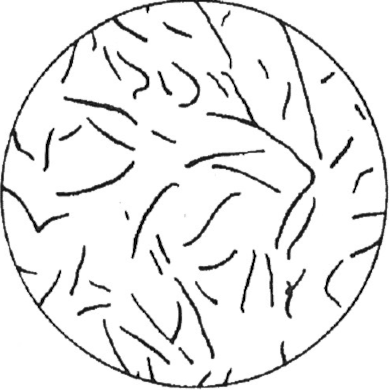
\includegraphics[scale=0.25]{pics/graphit_form1}
			\label{fig:LamellenGraphit}
			\caption*{\textbf{Form \uproman{1}}\\Lamellengraphit}
		\end{subfigure}\hfill
		\begin{subfigure}{0.33\textwidth}
			\centering
			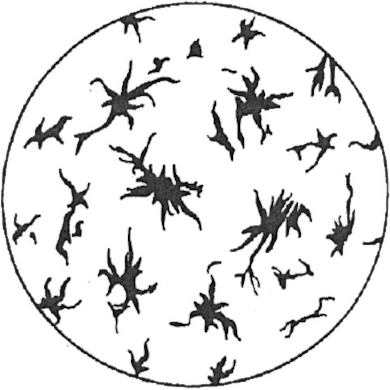
\includegraphics[scale=0.25]{pics/graphit_form2}
			\caption*{\textbf{Form \uproman{2}}\\Krabbengraphit}
		\end{subfigure}\hfill
		\begin{subfigure}{0.33\textwidth}
			\centering
			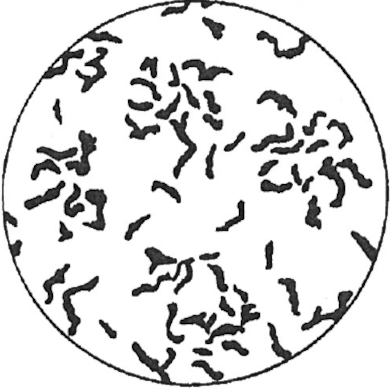
\includegraphics[scale=0.25]{pics/graphit_form3}
			\caption*{\textbf{Form \uproman{3}}\\Vermiculargraphit}
		\end{subfigure}
	\end{subfigure}
	\\\\\\
	\begin{subfigure}{1.0\linewidth}
		\begin{subfigure}[t]{0.33\textwidth}
			\centering
			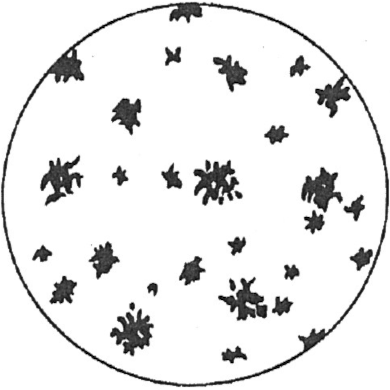
\includegraphics[scale=0.25]{pics/graphit_form4}
			\caption*{\textbf{Form \uproman{4}}\\ungleichförmiger\\Kugelgraphit}
		\end{subfigure}
		\begin{subfigure}[t]{0.33\textwidth}
			\centering
			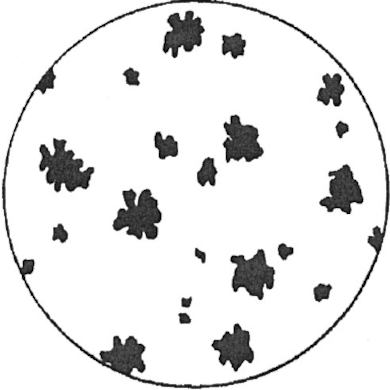
\includegraphics[scale=0.25]{pics/graphit_form5}
			\caption*{\textbf{Form \uproman{5}}\\gering ungleichf.\\Kugelgraphit }
		\end{subfigure}
		\begin{subfigure}[t]{0.33\textwidth}
			\centering
			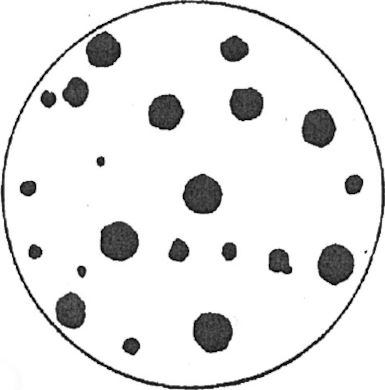
\includegraphics[scale=0.25]{pics/graphit_form6}
			\caption*{\textbf{Form \uproman{6}}\\Kugelgraphit}
		\end{subfigure}
	\end{subfigure}
	\caption{Typen von Gusseisen nach Form (\uproman{1} - \uproman{6}) der Graphitpartikelausbildung \cite[S.7]{ISO945}}
	\label{fig:GraphitTypes}
\end{figure}

\noindent Doch die Gusseisenwerkstoffe unterscheiden sich nicht nur hinsichtlich der Form und Struktur ihrer Graphiteinlagerungen, sondern vor allem auch in Bezug auf ihre damit unmittelbar in Zusammenhang stehenden mechanischen Eigenschaften, wie Zug- und Druckfestigkeit, dem Elastizitätsmodul, der Scherfestigkeit und weiterer Werkstoffkenndaten die, in Verbindung mit der Konstruktionsgeometrie die Qualität eines solchen Erzeugnisses ganz wesentlich beeinflussen. Das bedeutet, dass bei Kräfteeinwirkung je nach Art unterschiedliche Spannungskonzentrationen in den Graphiteinschlüssen entstehen und sich Gusseisenwerkstoffe unterschiedlicher Formklassen daher mehr oder weniger für bestimmte Verwendungszwecke eignen können. 
\\\\
\noindent Die wichtigsten Abnehmer von Gusseisenwerkstoffen sind der Straßenfahrzeugbau mit fast 60~\% sowie der Maschinenbau mit 25 bis 30~\% der gesamten Gusslieferungen \cite{BDGuss01}. Die Qualitätsanforderungen in diesen Branchen sind allgemein sehr hoch, jedoch wird gleichzeitig der  durch Substitution hervorgerufene Kostendruck auf die Hersteller stetig erhöht und zwingt diese zu Kostensenkungen im Bereich der Herstellkosten, bei gleichzeitiger Beibehaltung der Qualität. Ein weiterer Aspekt, der vor diesem Hintergrund für die Verwendung von Gusseisenwerkstoffen (vor allem Gusseisen mit Lamellengraphit) spricht, ist die Möglichkeit, diesen Zielkonflikt auf elegante Art und Weise zu lösen. Und zwar deshalb, weil der Kohlenstoffgehalt von 3 bis 4 Masseprozent im Gefüge zu wesentlichen Teilen als ausgeschiedener Graphit vorliegt und wegen der unterschiedlichen Dichte von Eisen und Graphit, 3,5 Masseprozent Kohlenstoff bis zu 11 Volumenprozent Graphit entsprechen können. Im Vergleich zu Stahl resultiert daraus eine immense Gewichts- und Kosteneinsparung, wobei die Unterschiede in den mechanischen Eigenschaften im Bedarfsfall durch entsprechende Werkstoffzugaben (Impfen) gewichtsneutral eliminiert werden können \cite{BDGuss02}.
\\\\
Die zur Beurteilung der Qualität von Gusseisenerzeugnissen maßgebliche Norm ist die DIN EN ISO 945-1. Genauso wie, je nach Art der Graphiteinlagerungen, eine grundsätzliche Einteilung in unterschiedliche Formklassen vorgenommen wird (siehe Abb. \ref{fig:GraphitTypes}), werden Gusseisenwerkstoffe mit Lamellengraphit zusätzlich in unterschiedliche Anordnungsklassen eingeteilt (siehe dazu auch Kapitel \ref{subsec:MethodenBestAnordnungsklassen} auf Seite \pageref{subsec:MethodenBestAnordnungsklassen}).
\\\\
Die Klassifizierung und Auswertung einer vorliegenden Werkstoffprobe erfolgt gemäß dieser Norm jedoch durch visuelle Auswertung, die von einer fachkundigen und entsprechend geschulten Fachkraft durchzuführen ist. Diese Vorgehensweise hat sich in der Praxis zwar über viele Jahre bewährt, ist aber dennoch fehleranfällig. Das ist sicherlich einer der Gründe dafür, weshalb moderne software-basierte Verfahren zur quantitativen Gefügeanalyse sich zu einem festen Bestandteil der heutigen metallographischen Praxis entwickelt hat, wenn auch diese Entwicklung noch lange nicht als abgeschlossen gelten kann \cite{schumann_oettel_2016}.
\\\\
Vor diesem Hintergrund ist auch die Software AMGuss entstanden, die von Gießereien zur schnellen und effizienten quantitativen Analyse der Mikrostruktur von Gusseisenwerkstoffen eingesetzt wird (vgl. dazu auch Kapitel \ref{sec:BestimmungMikrostrukturAMGuss}). Die Software  unterstützt  damit den Metallographen bei der Umsetzung der in \cite{ISO945} spezifizierten Anforderungen zur Analyse der Mikrostruktur von Gusseisenwerkstoffen und leistet somit einen wertvollen Beitrag zur Qualitätssicherung in Eisengießereien. Während das Programm Funktionalitäten zur Auswertung aller Formklassen (siehe Abb. \ref{fig:GraphitTypes}) anbietet, beschäftigt sich die vorliegend Arbeit ausschließlich mit Typ \uproman{1}, also der Analyse von Gusseisen mit Lamellengraphit oder GJL, wie der Werkstoff nach DIN EN 1561 auch bezeichnet wird. 




\chapter{Grundlagen}
\label{ch:Grundlagen}

\section{Klassifikation und Analyse von Gusseisenwerkstoffen mit Lamellengraphit}
\label{subsec:MethodenBestAnordnungsklassen}
Werden Gusseisenwerkstoffe mit Lamellengraphit nach DIN EN ISO 945-1 untersucht, müssen die darin enthaltenen Graphitbestandteile nach dem Bezeichnungssystem für die Klassifizierung von Graphit in Gusseisen klassifiziert  werden \cite[Seite 6]{ISO945}. Dazu bietet die Norm dem Metallographen sogenannte Richtreihenbilder an, anhand derer eine solche Klassifizierung durch visuelle Beurteilung durchzuführen ist.
\\\\
In der Formklasse Lamellengraphit (vgl. Abbildung \ref{fig:GraphitTypes} auf Seite \pageref{fig:GraphitTypes}) werden je nach Lage der Lamellen zueinander 5 verschiedene Anordnungsklassen (A - E) unterschiedenen, die in der folgenden Abbildung \ref{fig:Anordnungsklassen} dargestellt sind.

\begin{figure}[H]
	\centering
	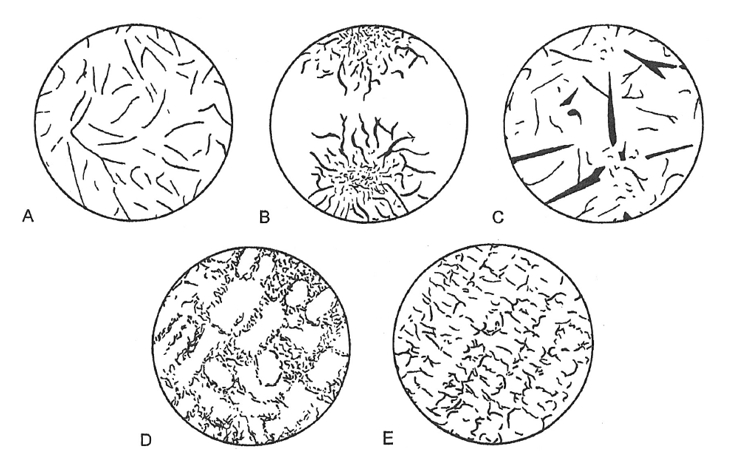
\includegraphics[scale=0.5]{pics/Anordnungsklassen}
	\caption{Richtreihenbilder für die Graphitanordnung\\ (Form \uproman{1} / Lamellengraphit) \cite{ISO945}}
	\label{fig:Anordnungsklassen}
\end{figure}

\noindent Diese Richtreihenbilder dienen also den entsprechenden Fachleuten in metallographischen Laboren dazu, die in einer Probe vorliegende morphologische Graphitstruktur durch visuellen Vergleich zu bestimmen. Somit ist das Ergebnis einer solchen Bestimmung niemals eindeutig, sondern hängt zwangsläufig von der subjektiven Einschätzung Metallographen ab \cite{ISO945}.
\\\\
\textcolor{red}{Welche Probleme ergeben sich daraus???}
\\\\

\section{Bildskalierung und Interpolationsverfahren}
\label{subsec:SkalierungUndInterpolation}

Unter Bildskalierung versteht man die Vergrößerung bzw. Verkleinerung von Bildern. Es handelt sich dabei um ein Standardverfahren, welches sowohl im Grafik- und Fotobereich als auch in der digitalen Bildverarbeitung sehr häufig zum Einsatz kommt und von Bildverarbeitungsprogrammen standardmäßig angeboten wird. Da die algorithmische Funktionsweise einer Bildskalierung für das Verständnis der in dieser Arbeit zu lösenden Problemstellung (siehe auch Kapitel \ref{sec:Problemstellung} auf Seite \pageref{sec:Problemstellung}) von zentraler Bedeutung ist, wird diese nun hier genauer Untersucht und beschrieben.
\\\\
Das grundsätzliche Problem bei der Skalierung von Bildern, soll durch Abbildung \ref{fig:ScalingProblem} verdeutlicht werden. Zu sehen ist links ein Bild mit ($4\times 4$) Pixeln (orange) und rechts das durch Skalierung erzeugte Bild. Die neue Position eines beliebigen Originalpixels im neu erzeugten (skalierten) Bild ergibt sich durch Multiplikation der ursprünglichen Position mit dem Skalierungsfaktor ($\lambda$).
\begin{figure}[H]
	\centering
		\begin{tikzpicture}[x=0.75pt,y=0.75pt,yscale=-1,xscale=1, scale=0.9, every node/.style={scale=0.9}]
			%uncomment if require: \path (0,300); %set diagram left start at 0, 	and has height of 300
			
			%Shape: Rectangle [id:dp33493272980948086] 
			\draw  [color={rgb, 255:red, 255; green, 255; blue, 255 }  ,draw opacity=1 ][fill={rgb, 255:red, 155; green, 155; blue, 155 }  ,fill opacity=1 ] (240,53.85) -- (400,53.85) -- (400,213.85) -- (240,213.85) -- cycle ;
			%Shape: Grid [id:dp5166847032058127] 
			\draw  [draw opacity=0][fill={rgb, 255:red, 126; green, 211; blue, 33 }  ,fill opacity=1 ][line width=1.5]  (35.38,93.85) -- (116.38,93.85) -- (116.38,174.85) -- (35.38,174.85) -- cycle ; \draw  [line width=1.5]  (35.38,93.85) -- (35.38,174.85)(55.38,93.85) -- (55.38,174.85)(75.38,93.85) -- (75.38,174.85)(95.38,93.85) -- (95.38,174.85)(115.38,93.85) -- (115.38,174.85) ; \draw  [line width=1.5]  (35.38,93.85) -- (116.38,93.85)(35.38,113.85) -- (116.38,113.85)(35.38,133.85) -- (116.38,133.85)(35.38,153.85) -- (116.38,153.85)(35.38,173.85) -- (116.38,173.85) ; \draw  [line width=1.5]   ;
			%Right Arrow [id:dp7963578241503881] 
			\draw  [line width=1.5]  (139.38,125) -- (172.98,125) -- (172.98,116) -- (195.38,134) -- (172.98,152) -- (172.98,143) -- (139.38,143) -- cycle ;
			%Shape: Grid [id:dp813346916234577] 
			\draw  [draw opacity=0][line width=1.5]  (240,53.85) -- (400.38,53.85) -- (400.38,214.85) -- (240,214.85) -- cycle ; \draw  [color={rgb, 255:red, 0; green, 0; blue, 0 }  ,draw opacity=1 ][line width=1.5]  (240,53.85) -- (240,214.85)(260,53.85) -- (260,214.85)(280,53.85) -- (280,214.85)(300,53.85) -- (300,214.85)(320,53.85) -- (320,214.85)(340,53.85) -- (340,214.85)(360,53.85) -- (360,214.85)(380,53.85) -- (380,214.85)(400,53.85) -- (400,214.85) ; \draw  [color={rgb, 255:red, 0; green, 0; blue, 0 }  ,draw opacity=1 ][line width=1.5]  (240,53.85) -- (400.38,53.85)(240,73.85) -- (400.38,73.85)(240,93.85) -- (400.38,93.85)(240,113.85) -- (400.38,113.85)(240,133.85) -- (400.38,133.85)(240,153.85) -- (400.38,153.85)(240,173.85) -- (400.38,173.85)(240,193.85) -- (400.38,193.85)(240,213.85) -- (400.38,213.85) ; \draw  [color={rgb, 255:red, 0; green, 0; blue, 0 }  ,draw opacity=1 ][line width=1.5]   ;
			%Shape: Rectangle [id:dp7852221432702648] 
			\draw  [fill={rgb, 255:red, 126; green, 211; blue, 33 }  ,fill opacity=1 ][line width=1.5]  (240,53.85) -- (260,53.85) -- (260,73.85) -- (240,73.85) -- cycle ;
			%Shape: Rectangle [id:dp316493263782738] 
			\draw  [fill={rgb, 255:red, 126; green, 211; blue, 33 }  ,fill opacity=1 ][line width=1.5]  (360,53.85) -- (380,53.85) -- (380,73.85) -- (360,73.85) -- cycle ;
			%Shape: Rectangle [id:dp9150879931583693] 
			\draw  [fill={rgb, 255:red, 126; green, 211; blue, 33 }  ,fill opacity=1 ][line width=1.5]  (280,53.85) -- (300,53.85) -- (300,73.85) -- (280,73.85) -- cycle ;
			%Shape: Rectangle [id:dp21254213121480348] 
			\draw  [fill={rgb, 255:red, 126; green, 211; blue, 33 }  ,fill opacity=1 ][line width=1.5]  (320,53.85) -- (340,53.85) -- (340,73.85) -- (320,73.85) -- cycle ;
			%Shape: Rectangle [id:dp9138059724854111] 
			\draw  [fill={rgb, 255:red, 126; green, 211; blue, 33 }  ,fill opacity=1 ][line width=1.5]  (240,93.85) -- (260,93.85) -- (260,113.85) -- (240,113.85) -- cycle ;
			%Shape: Rectangle [id:dp8385734790799879] 
			\draw  [fill={rgb, 255:red, 126; green, 211; blue, 33 }  ,fill opacity=1 ][line width=1.5]  (360,93.85) -- (380,93.85) -- (380,113.85) -- (360,113.85) -- cycle ;
			%Shape: Rectangle [id:dp0266783762407925] 
			\draw  [fill={rgb, 255:red, 126; green, 211; blue, 33 }  ,fill opacity=1 ][line width=1.5]  (280,93.85) -- (300,93.85) -- (300,113.85) -- (280,113.85) -- cycle ;
			%Shape: Rectangle [id:dp8765432738424186] 
			\draw  [fill={rgb, 255:red, 126; green, 211; blue, 33 }  ,fill opacity=1 ][line width=1.5]  (320,93.85) -- (340,93.85) -- (340,113.85) -- (320,113.85) -- cycle ;
			%Shape: Rectangle [id:dp3683961028684497] 
			\draw  [fill={rgb, 255:red, 126; green, 211; blue, 33 }  ,fill opacity=1 ][line width=1.5]  (240,133.85) -- (260,133.85) -- (260,153.85) -- (240,153.85) -- cycle ;
			%Shape: Rectangle [id:dp17023134792901806] 
			\draw  [fill={rgb, 255:red, 126; green, 211; blue, 33 }  ,fill opacity=1 ][line width=1.5]  (360,133.85) -- (380,133.85) -- (380,153.85) -- (360,153.85) -- cycle ;
			%Shape: Rectangle [id:dp30885139351862023] 
			\draw  [fill={rgb, 255:red, 126; green, 211; blue, 33 }  ,fill opacity=1 ][line width=1.5]  (280,133.85) -- (300,133.85) -- (300,153.85) -- (280,153.85) -- cycle ;
			%Shape: Rectangle [id:dp2063497064425942] 
			\draw  [fill={rgb, 255:red, 126; green, 211; blue, 33 }  ,fill opacity=1 ][line width=1.5]  (320,133.85) -- (340,133.85) -- (340,153.85) -- (320,153.85) -- cycle ;
			%Shape: Rectangle [id:dp7893916008859733] 
			\draw  [fill={rgb, 255:red, 126; green, 211; blue, 33 }  ,fill opacity=1 ][line width=1.5]  (240,173.85) -- (260,173.85) -- (260,193.85) -- (240,193.85) -- cycle ;
			%Shape: Rectangle [id:dp03560102427440881] 
			\draw  [fill={rgb, 255:red, 126; green, 211; blue, 33 }  ,fill opacity=1 ][line width=1.5]  (360,173.85) -- (380,173.85) -- (380,193.85) -- (360,193.85) -- cycle ;
			%Shape: Rectangle [id:dp5475282364153556] 
			\draw  [fill={rgb, 255:red, 126; green, 211; blue, 33 }  ,fill opacity=1 ][line width=1.5]  (280,173.85) -- (300,173.85) -- (300,193.85) -- (280,193.85) -- cycle ;
			%Shape: Rectangle [id:dp34756519033919797] 
			\draw  [fill={rgb, 255:red, 126; green, 211; blue, 33 }  ,fill opacity=1 ][line width=1.5]  (320,173.85) -- (340,173.85) -- (340,193.85) -- (320,193.85) -- cycle ;
			%Straight Lines [id:da27131202915211117] 
			\draw [color={rgb, 255:red, 0; green, 0; blue, 0 }  ,draw opacity=1 ][line width=1.5]    (17.38,69.85) -- (46,69.85) -- (88,69.85) -- (142.38,69.85) ;
			\draw [shift={(145.38,69.85)}, rotate = 180] [color={rgb, 255:red, 0; green, 0; blue, 0 }  ,draw opacity=1 ][line width=1.5]    (14.21,-4.28) .. controls (9.04,-1.82) and (4.3,-0.39) .. (0,0) .. controls (4.3,0.39) and (9.04,1.82) .. (14.21,4.28)   ;
			%Straight Lines [id:da0003577742395167727] 
			\draw [color={rgb, 255:red, 0; green, 0; blue, 0 }  ,draw opacity=1 ][line width=1.5]    (17.38,69.85) -- (17.38,197.85) ;
			\draw [shift={(17.38,200.85)}, rotate = 270] [color={rgb, 255:red, 0; green, 0; blue, 0 }  ,draw opacity=1 ][line width=1.5]    (14.21,-4.28) .. controls (9.04,-1.82) and (4.3,-0.39) .. (0,0) .. controls (4.3,0.39) and (9.04,1.82) .. (14.21,4.28)   ;
			%Straight Lines [id:da8167500493181958] 
			\draw [fill={rgb, 255:red, 0; green, 0; blue, 0 }  ,fill opacity=1 ][line width=1.5]    (218.38,26.85) -- (446.38,26.85) ;
			\draw [shift={(449.38,26.85)}, rotate = 180] [color={rgb, 255:red, 0; green, 0; blue, 0 }  ][line width=1.5]    (14.21,-4.28) .. controls (9.04,-1.82) and (4.3,-0.39) .. (0,0) .. controls (4.3,0.39) and (9.04,1.82) .. (14.21,4.28)   ;
			%Straight Lines [id:da5628538454694642] 
			\draw [color={rgb, 255:red, 0; green, 0; blue, 0 }  ,draw opacity=1 ][line width=1.5]    (218.38,26.85) -- (218.38,243.85) ;
			\draw [shift={(218.38,246.85)}, rotate = 270] [color={rgb, 255:red, 0; green, 0; blue, 0 }  ,draw opacity=1 ][line width=1.5]    (14.21,-4.28) .. controls (9.04,-1.82) and (4.3,-0.39) .. (0,0) .. controls (4.3,0.39) and (9.04,1.82) .. (14.21,4.28)   ;
			
			% Text Node
			\draw (142.29,125) node [anchor=north west][inner sep=0.75pt]  [font=\normalsize,xslant=0.03] [align=left] {$\displaystyle \lambda $\textbf{ = 2}};
			% Text Node
			\draw (91,191) node [anchor=north west][inner sep=0.75pt]   [align=left] {{\footnotesize \textcolor[rgb]{0,0,0}{$\displaystyle \lambda $}\textcolor[rgb]{0,0,0}{\textbf{: Skalierungsfaktor}}}};
			% Text Node
			\draw (23,96) node [anchor=north west][inner sep=0.75pt]   [align=left] {0};
			% Text Node
			\draw (23,116) node [anchor=north west][inner sep=0.75pt]   [align=left] {1};
			% Text Node
			\draw (23,136) node [anchor=north west][inner sep=0.75pt]   [align=left] {2};
			% Text Node
			\draw (23,157) node [anchor=north west][inner sep=0.75pt]   [align=left] {3};
			% Text Node
			\draw (40,75) node [anchor=north west][inner sep=0.75pt]   [align=left] {0};
			% Text Node
			\draw (60,75) node [anchor=north west][inner sep=0.75pt]   [align=left] {1};
			% Text Node
			\draw (80,75) node [anchor=north west][inner sep=0.75pt]   [align=left] {2};
			% Text Node
			\draw (101,75) node [anchor=north west][inner sep=0.75pt]   [align=left] {3};
			% Text Node
			\draw (150,61) node [anchor=north west][inner sep=0.75pt]   [align=left] {\textbf{x}};
			% Text Node
			\draw (13,204) node [anchor=north west][inner sep=0.75pt]   [align=left] {\textbf{y}};
			% Text Node
			\draw (244,34) node [anchor=north west][inner sep=0.75pt]   [align=left] {0};
			% Text Node
			\draw (264,34) node [anchor=north west][inner sep=0.75pt]   [align=left] {1};
			% Text Node
			\draw (284,34) node [anchor=north west][inner sep=0.75pt]   [align=left] {2};
			% Text Node
			\draw (305,34) node [anchor=north west][inner sep=0.75pt]   [align=left] {3};
			% Text Node
			\draw (325,34) node [anchor=north west][inner sep=0.75pt]   [align=left] {4};
			% Text Node
			\draw (345,34) node [anchor=north west][inner sep=0.75pt]   [align=left] {5};
			% Text Node
			\draw (365,34) node [anchor=north west][inner sep=0.75pt]   [align=left] {6};
			% Text Node
			\draw (384,34) node [anchor=north west][inner sep=0.75pt]   [align=left] {7};
			% Text Node
			\draw (227,56) node [anchor=north west][inner sep=0.75pt]   [align=left] {0};
			% Text Node
			\draw (227,76) node [anchor=north west][inner sep=0.75pt]   [align=left] {1};
			% Text Node
			\draw (227,96) node [anchor=north west][inner sep=0.75pt]   [align=left] {2};
			% Text Node
			\draw (227,117) node [anchor=north west][inner sep=0.75pt]   [align=left] {3};
			% Text Node
			\draw (227,137) node [anchor=north west][inner sep=0.75pt]   [align=left] {4};
			% Text Node
			\draw (227,157) node [anchor=north west][inner sep=0.75pt]   [align=left] {5};
			% Text Node
			\draw (227,176) node [anchor=north west][inner sep=0.75pt]   [align=left] {6};
			% Text Node
			\draw (227,197) node [anchor=north west][inner sep=0.75pt]   [align=left] {7};
			% Text Node
			\draw (457,17) node [anchor=north west][inner sep=0.75pt]   [align=left] {\textbf{x}};
			% Text Node
			\draw (214,248) node [anchor=north west][inner sep=0.75pt]   [align=left] {\textbf{y}};
		\end{tikzpicture}
	\caption{Darstellung der Notwendigkeit von\\ Interpolationsverfahren bei der Bildskalierung}
	\label{fig:ScalingProblem}
\end{figure}

\noindent Genauer ausgedrückt handelt es sich bei den Lücken um undefinierte Pixel, da sich die Pixelmenge proportional zum Skalierungsfaktor ebenfalls verändert. Bei Skalierungsfaktoren kleiner 1 verhält es sich genau umgekehrt und die Anzahl der Pixel im Ergebnisbild verringert sich entsprechend.
\\\\
\noindent Zur Lösung dieses Problems wurden verschiedene Interpolationsalgorithmen entwickelt. Diese verfolgen alle das Ziel, die sich ergebende Differenz der Pixelanzahl auszugleichen und die Bildqualität dadurch möglichst gut zu erhalten. Dabei werden also die Farbwerte der grauen (undefinierten) Pixel aus den Farbwerten der umliegenden Pixel auf jeweils unterschiedliche Art approximiert. Es liegt jedoch auf der Hand, das ein solchen Verfahren die Details eines gegebenen Originalbildes nie 100\%-ig erhalten kann. So können zwar für viele praktische Anwendungsfälle im Grafik- oder Fotobereich sehr gute Ergebnisse erzielt werden, weil das menschliche Auge diese Abweichungen nicht erkennen kann. Allerdings erweist sich die Interpolation im Bereich der bildbasierten Materialstrukturanalyse als problematisch, da sich  die zu analysierenden Strukturen durch die Interpolation verändern und somit die Messergebnisse verfälscht werden. 
\\\\
\noindent Dieser Zusammenhang wird nun Anhand der bilinearen Interpolation einmal genauer erklärt, damit sicher der Leser ein besseres Bild davon machen kann. Dabei handelt es sich um ein sehr einfaches Verfahren, bei dem zur Bestimmung unbestimmter Pixel nach der Skalierung, deren Farbwerte (RGB) durch lineare Interpolation in X- und Y-Richtung berechnet werden. Als Beispiel dient folgende Situation, die in Abbildung \ref{fig:BilinearInterpolation1} dargestellt ist.

\begin{figure}[H]
	\centering
	\begin{tikzpicture}[x=0.75pt,y=0.75pt,yscale=-1,xscale=1, scale=1.2, every node/.style={scale=1.2}]
		%uncomment if require: \path (0,374); %set diagram left start at 0, and has height of 374
		
		%Shape: Grid [id:dp6031282918603735] 
		\draw  [draw opacity=0][line width=1.5]  (300.38,50.85) -- (481.38,50.85) -- (481.38,231.85) -- (300.38,231.85) -- cycle ; \draw  [color={rgb, 255:red, 0; green, 0; blue, 0 }  ,draw opacity=1 ][line width=1.5]  (300.38,50.85) -- (300.38,231.85)(330.38,50.85) -- (330.38,231.85)(360.38,50.85) -- (360.38,231.85)(390.38,50.85) -- (390.38,231.85)(420.38,50.85) -- (420.38,231.85)(450.38,50.85) -- (450.38,231.85)(480.38,50.85) -- (480.38,231.85) ; \draw  [color={rgb, 255:red, 0; green, 0; blue, 0 }  ,draw opacity=1 ][line width=1.5]  (300.38,50.85) -- (481.38,50.85)(300.38,80.85) -- (481.38,80.85)(300.38,110.85) -- (481.38,110.85)(300.38,140.85) -- (481.38,140.85)(300.38,170.85) -- (481.38,170.85)(300.38,200.85) -- (481.38,200.85)(300.38,230.85) -- (481.38,230.85) ; \draw  [color={rgb, 255:red, 0; green, 0; blue, 0 }  ,draw opacity=1 ][line width=1.5]   ;
		%Shape: Axis 2D [id:dp12421444962330219] 
		\draw  (283.56,4.16) -- (283.56,260.85)(506.38,29.83) -- (258.81,29.83) (288.56,253.85) -- (283.56,260.85) -- (278.56,253.85) (499.38,24.83) -- (506.38,29.83) -- (499.38,34.83)  ;
		%Shape: Axis 2D [id:dp5582126406856516] 
		\draw  (43.86,14.16) -- (43.86,166.85)(188.38,29.43) -- (27.81,29.43) (48.86,159.85) -- (43.86,166.85) -- (38.86,159.85) (181.38,24.43) -- (188.38,29.43) -- (181.38,34.43)  ;
		%Shape: Grid [id:dp6426300130896345] 
		\draw  [draw opacity=0][line width=2.25]  (62,51) -- (152.38,51) -- (152.38,141.85) -- (62,141.85) -- cycle ; \draw  [line width=2.25]  (62,51) -- (62,141.85)(92,51) -- (92,141.85)(122,51) -- (122,141.85)(152,51) -- (152,141.85) ; \draw  [line width=2.25]  (62,51) -- (152.38,51)(62,81) -- (152.38,81)(62,111) -- (152.38,111)(62,141) -- (152.38,141) ; \draw  [line width=2.25]   ;
		%Shape: Rectangle [id:dp13871600656081773] 
		\draw  [fill={rgb, 255:red, 245; green, 166; blue, 35 }  ,fill opacity=1 ][line width=1.5]  (92,51) -- (122,51) -- (122,81) -- (92,81) -- cycle ;
		%Shape: Rectangle [id:dp09914050619225745] 
		\draw  [fill={rgb, 255:red, 245; green, 166; blue, 35 }  ,fill opacity=1 ][line width=1.5]  (122,81) -- (152,81) -- (152,111) -- (122,111) -- cycle ;
		%Shape: Rectangle [id:dp7354425170625416] 
		\draw  [fill={rgb, 255:red, 245; green, 166; blue, 35 }  ,fill opacity=1 ][line width=1.5]  (122,111) -- (152,111) -- (152,141) -- (122,141) -- cycle ;
		%Shape: Rectangle [id:dp8022069903462297] 
		\draw  [fill={rgb, 255:red, 245; green, 166; blue, 35 }  ,fill opacity=1 ][line width=1.5]  (62,111) -- (92,111) -- (92,141) -- (62,141) -- cycle ;
		%Shape: Rectangle [id:dp5675136532554508] 
		\draw  [fill={rgb, 255:red, 245; green, 166; blue, 35 }  ,fill opacity=1 ][line width=1.5]  (92,111) -- (122,111) -- (122,141) -- (92,141) -- cycle ;
		%Shape: Rectangle [id:dp26546030668596743] 
		\draw  [fill={rgb, 255:red, 126; green, 211; blue, 33 }  ,fill opacity=1 ][line width=1.5]  (122,51) -- (152,51) -- (152,81) -- (122,81) -- cycle ;
		%Shape: Rectangle [id:dp31022250660119444] 
		\draw  [fill={rgb, 255:red, 126; green, 211; blue, 33 }  ,fill opacity=1 ][line width=1.5]  (92,81) -- (122,81) -- (122,111) -- (92,111) -- cycle ;
		%Shape: Rectangle [id:dp1632256531496281] 
		\draw  [fill={rgb, 255:red, 126; green, 211; blue, 33 }  ,fill opacity=1 ][line width=1.5]  (62,51) -- (92,51) -- (92,81) -- (62,81) -- cycle ;
		%Shape: Rectangle [id:dp36586491405776467] 
		\draw  [fill={rgb, 255:red, 126; green, 211; blue, 33 }  ,fill opacity=1 ][line width=1.5]  (62,81) -- (92,81) -- (92,111) -- (62,111) -- cycle ;
		%Shape: Rectangle [id:dp09483486001396602] 
		\draw  [fill={rgb, 255:red, 245; green, 166; blue, 35 }  ,fill opacity=1 ][line width=1.5]  (360.38,50.85) -- (390.38,50.85) -- (390.38,80.85) -- (360.38,80.85) -- cycle ;
		%Shape: Rectangle [id:dp8722790379045016] 
		\draw  [fill={rgb, 255:red, 245; green, 166; blue, 35 }  ,fill opacity=1 ][line width=1.5]  (420.38,110.85) -- (450.38,110.85) -- (450.38,140.85) -- (420.38,140.85) -- cycle ;
		%Shape: Rectangle [id:dp3090077325311579] 
		\draw  [fill={rgb, 255:red, 245; green, 166; blue, 35 }  ,fill opacity=1 ][line width=1.5]  (420.38,170.85) -- (450.38,170.85) -- (450.38,200.85) -- (420.38,200.85) -- cycle ;
		%Shape: Rectangle [id:dp39265423932322685] 
		\draw  [fill={rgb, 255:red, 245; green, 166; blue, 35 }  ,fill opacity=1 ][line width=1.5]  (300.38,170.85) -- (330.38,170.85) -- (330.38,200.85) -- (300.38,200.85) -- cycle ;
		%Shape: Rectangle [id:dp309527828572457] 
		\draw  [fill={rgb, 255:red, 245; green, 166; blue, 35 }  ,fill opacity=1 ][line width=1.5]  (360.38,170.85) -- (390.38,170.85) -- (390.38,200.85) -- (360.38,200.85) -- cycle ;
		%Shape: Rectangle [id:dp43382954399056994] 
		\draw  [fill={rgb, 255:red, 126; green, 211; blue, 33 }  ,fill opacity=1 ][line width=1.5]  (420.38,50.85) -- (450.38,50.85) -- (450.38,80.85) -- (420.38,80.85) -- cycle ;
		%Shape: Rectangle [id:dp5113204315472576] 
		\draw  [fill={rgb, 255:red, 126; green, 211; blue, 33 }  ,fill opacity=1 ][line width=1.5]  (360.38,110.85) -- (390.38,110.85) -- (390.38,140.85) -- (360.38,140.85) -- cycle ;
		%Shape: Rectangle [id:dp06279947117329954] 
		\draw  [fill={rgb, 255:red, 126; green, 211; blue, 33 }  ,fill opacity=1 ][line width=1.5]  (300.38,50.85) -- (330.38,50.85) -- (330.38,80.85) -- (300.38,80.85) -- cycle ;
		%Shape: Rectangle [id:dp7495389450561212] 
		\draw  [fill={rgb, 255:red, 126; green, 211; blue, 33 }  ,fill opacity=1 ][line width=1.5]  (300.38,110.85) -- (330.38,110.85) -- (330.38,140.85) -- (300.38,140.85) -- cycle ;
		%Shape: Rectangle [id:dp3179677452191165] 
		\draw  [color={rgb, 255:red, 0; green, 0; blue, 0 }  ,draw opacity=1 ][fill={rgb, 255:red, 185; green, 188; blue, 34 }  ,fill opacity=1 ][line width=1.5]  (330.38,50.85) -- (360.38,50.85) -- (360.38,80.85) -- (330.38,80.85) -- cycle ;
		%Shape: Rectangle [id:dp02520564590269525] 
		\draw  [color={rgb, 255:red, 0; green, 0; blue, 0 }  ,draw opacity=1 ][fill={rgb, 255:red, 185; green, 188; blue, 34 }  ,fill opacity=1 ][line width=1.5]  (390.38,50.85) -- (420.38,50.85) -- (420.38,80.85) -- (390.38,80.85) -- cycle ;
		%Shape: Rectangle [id:dp41456521365377197] 
		\draw  [color={rgb, 255:red, 0; green, 0; blue, 0 }  ,draw opacity=1 ][fill={rgb, 255:red, 185; green, 188; blue, 34 }  ,fill opacity=1 ][line width=1.5]  (360.38,80.85) -- (390.38,80.85) -- (390.38,110.85) -- (360.38,110.85) -- cycle ;
		%Shape: Rectangle [id:dp7715421317421746] 
		\draw  [color={rgb, 255:red, 0; green, 0; blue, 0 }  ,draw opacity=1 ][fill={rgb, 255:red, 185; green, 188; blue, 34 }  ,fill opacity=1 ][line width=1.5]  (420.38,80.85) -- (450.38,80.85) -- (450.38,110.85) -- (420.38,110.85) -- cycle ;
		%Shape: Rectangle [id:dp6537803831672764] 
		\draw  [color={rgb, 255:red, 0; green, 0; blue, 0 }  ,draw opacity=1 ][fill={rgb, 255:red, 185; green, 188; blue, 34 }  ,fill opacity=1 ][line width=1.5]  (390.38,110.85) -- (420.38,110.85) -- (420.38,140.85) -- (390.38,140.85) -- cycle ;
		%Shape: Rectangle [id:dp694492919060651] 
		\draw  [color={rgb, 255:red, 0; green, 0; blue, 0 }  ,draw opacity=1 ][fill={rgb, 255:red, 185; green, 188; blue, 34 }  ,fill opacity=1 ][line width=1.5]  (390.38,80.85) -- (420.38,80.85) -- (420.38,110.85) -- (390.38,110.85) -- cycle ;
		%Shape: Rectangle [id:dp8749183811880095] 
		\draw  [color={rgb, 255:red, 0; green, 0; blue, 0 }  ,draw opacity=1 ][fill={rgb, 255:red, 185; green, 188; blue, 34 }  ,fill opacity=1 ][line width=1.5]  (300.38,140.85) -- (330.38,140.85) -- (330.38,170.85) -- (300.38,170.85) -- cycle ;
		%Shape: Rectangle [id:dp15019771324119735] 
		\draw  [color={rgb, 255:red, 0; green, 0; blue, 0 }  ,draw opacity=1 ][fill={rgb, 255:red, 185; green, 188; blue, 34 }  ,fill opacity=1 ][line width=1.5]  (360.38,140.85) -- (390.38,140.85) -- (390.38,170.85) -- (360.38,170.85) -- cycle ;
		%Shape: Rectangle [id:dp8886413553682353] 
		\draw  [color={rgb, 255:red, 0; green, 0; blue, 0 }  ,draw opacity=1 ][fill={rgb, 255:red, 185; green, 188; blue, 34 }  ,fill opacity=1 ][line width=1.5]  (330.38,140.85) -- (360.38,140.85) -- (360.38,170.85) -- (330.38,170.85) -- cycle ;
		%Shape: Rectangle [id:dp18893376895528624] 
		\draw  [fill={rgb, 255:red, 245; green, 166; blue, 35 }  ,fill opacity=1 ][line width=1.5]  (420.38,140.85) -- (450.38,140.85) -- (450.38,170.85) -- (420.38,170.85) -- cycle ;
		%Shape: Rectangle [id:dp8401086030387102] 
		\draw  [fill={rgb, 255:red, 245; green, 166; blue, 35 }  ,fill opacity=1 ][line width=1.5]  (390.38,170.85) -- (420.38,170.85) -- (420.38,200.85) -- (390.38,200.85) -- cycle ;
		%Shape: Rectangle [id:dp5023664828243175] 
		\draw  [fill={rgb, 255:red, 245; green, 166; blue, 35 }  ,fill opacity=1 ][line width=1.5]  (330.38,170.85) -- (360.38,170.85) -- (360.38,200.85) -- (330.38,200.85) -- cycle ;
		%Shape: Rectangle [id:dp4926347479761316] 
		\draw  [fill={rgb, 255:red, 126; green, 211; blue, 33 }  ,fill opacity=1 ][line width=1.5]  (300.38,80.85) -- (330.38,80.85) -- (330.38,110.85) -- (300.38,110.85) -- cycle ;
		%Shape: Rectangle [id:dp03314094385373201] 
		\draw  [fill={rgb, 255:red, 126; green, 211; blue, 33 }  ,fill opacity=1 ][line width=1.5]  (330.38,110.85) -- (360.38,110.85) -- (360.38,140.85) -- (330.38,140.85) -- cycle ;
		%Shape: Rectangle [id:dp31700461022402926] 
		\draw  [color={rgb, 255:red, 0; green, 0; blue, 0 }  ,draw opacity=1 ][fill={rgb, 255:red, 155; green, 199; blue, 33 }  ,fill opacity=1 ][line width=1.5]  (330.38,80.85) -- (360.38,80.85) -- (360.38,110.85) -- (330.38,110.85) -- cycle ;
		%Shape: Rectangle [id:dp17649729390737434] 
		\draw  [color={rgb, 255:red, 0; green, 0; blue, 0 }  ,draw opacity=1 ][fill={rgb, 255:red, 215; green, 177; blue, 34 }  ,fill opacity=1 ][line width=1.5]  (390.38,140.85) -- (420.38,140.85) -- (420.38,170.85) -- (390.38,170.85) -- cycle ;
		%Right Arrow [id:dp33270781304422914] 
		\draw  [line width=1.5]  (185,86) -- (227,86) -- (227,76) -- (255,96) -- (227,116) -- (227,106) -- (185,106) -- cycle ;
		%Shape: Rectangle [id:dp24983247014857224] 
		\draw  [fill={rgb, 255:red, 126; green, 211; blue, 33 }  ,fill opacity=1 ][line width=1.5]  (450.38,50.85) -- (480.38,50.85) -- (480.38,80.85) -- (450.38,80.85) -- cycle ;
		%Shape: Rectangle [id:dp35849526261121356] 
		\draw  [fill={rgb, 255:red, 245; green, 166; blue, 35 }  ,fill opacity=1 ][line width=1.5]  (450.38,110.85) -- (480.38,110.85) -- (480.38,140.85) -- (450.38,140.85) -- cycle ;
		%Shape: Rectangle [id:dp1351111821765797] 
		\draw  [fill={rgb, 255:red, 245; green, 166; blue, 35 }  ,fill opacity=1 ][line width=1.5]  (450.38,170.85) -- (480.38,170.85) -- (480.38,200.85) -- (450.38,200.85) -- cycle ;
		%Shape: Rectangle [id:dp5617796085771564] 
		\draw  [color={rgb, 255:red, 0; green, 0; blue, 0 }  ,draw opacity=1 ][fill={rgb, 255:red, 185; green, 188; blue, 34 }  ,fill opacity=1 ][line width=1.5]  (450.38,80.85) -- (480.38,80.85) -- (480.38,110.85) -- (450.38,110.85) -- cycle ;
		%Shape: Rectangle [id:dp6849626334604124] 
		\draw  [fill={rgb, 255:red, 245; green, 166; blue, 35 }  ,fill opacity=1 ][line width=1.5]  (450.38,140.85) -- (480.38,140.85) -- (480.38,170.85) -- (450.38,170.85) -- cycle ;
		%Shape: Rectangle [id:dp4423643524339804] 
		\draw  [fill={rgb, 255:red, 245; green, 166; blue, 35 }  ,fill opacity=1 ][line width=1.5]  (420.38,200.85) -- (450.38,200.85) -- (450.38,230.85) -- (420.38,230.85) -- cycle ;
		%Shape: Rectangle [id:dp9844308475991588] 
		\draw  [fill={rgb, 255:red, 245; green, 166; blue, 35 }  ,fill opacity=1 ][line width=1.5]  (300.38,200.85) -- (330.38,200.85) -- (330.38,230.85) -- (300.38,230.85) -- cycle ;
		%Shape: Rectangle [id:dp19330105393002595] 
		\draw  [fill={rgb, 255:red, 245; green, 166; blue, 35 }  ,fill opacity=1 ][line width=1.5]  (360.38,200.85) -- (390.38,200.85) -- (390.38,230.85) -- (360.38,230.85) -- cycle ;
		%Shape: Rectangle [id:dp719400766119336] 
		\draw  [fill={rgb, 255:red, 245; green, 166; blue, 35 }  ,fill opacity=1 ][line width=1.5]  (390.38,200.85) -- (420.38,200.85) -- (420.38,230.85) -- (390.38,230.85) -- cycle ;
		%Shape: Rectangle [id:dp3277584194542974] 
		\draw  [fill={rgb, 255:red, 245; green, 166; blue, 35 }  ,fill opacity=1 ][line width=1.5]  (330.38,200.85) -- (360.38,200.85) -- (360.38,230.85) -- (330.38,230.85) -- cycle ;
		%Shape: Rectangle [id:dp5673130666239078] 
		\draw  [fill={rgb, 255:red, 245; green, 166; blue, 35 }  ,fill opacity=1 ][line width=1.5]  (450.38,200.85) -- (480.38,200.85) -- (480.38,230.85) -- (450.38,230.85) -- cycle ;
		%Left Right Arrow [id:dp10603987349893162] 
		\draw  [color={rgb, 255:red, 255; green, 255; blue, 255 }  ,draw opacity=1 ] (334.19,65.85) -- (339.79,58.43) -- (339.79,62.14) -- (350.98,62.14) -- (350.98,58.43) -- (356.57,65.85) -- (350.98,73.28) -- (350.98,69.56) -- (339.79,69.56) -- (339.79,73.28) -- cycle ;
		%Left Right Arrow [id:dp4851771954641114] 
		\draw  [color={rgb, 255:red, 255; green, 255; blue, 255 }  ,draw opacity=1 ] (394.19,65.85) -- (399.79,58.43) -- (399.79,62.14) -- (410.98,62.14) -- (410.98,58.43) -- (416.57,65.85) -- (410.98,73.28) -- (410.98,69.56) -- (399.79,69.56) -- (399.79,73.28) -- cycle ;
		%Left Right Arrow [id:dp46535515779583203] 
		\draw  [color={rgb, 255:red, 255; green, 255; blue, 255 }  ,draw opacity=1 ] (334.19,185.85) -- (339.79,178.43) -- (339.79,182.14) -- (350.98,182.14) -- (350.98,178.43) -- (356.57,185.85) -- (350.98,193.28) -- (350.98,189.56) -- (339.79,189.56) -- (339.79,193.28) -- cycle ;
		%Left Right Arrow [id:dp0388460015786245] 
		\draw  [color={rgb, 255:red, 255; green, 255; blue, 255 }  ,draw opacity=1 ] (394.19,185.85) -- (399.79,178.43) -- (399.79,182.14) -- (410.98,182.14) -- (410.98,178.43) -- (416.57,185.85) -- (410.98,193.28) -- (410.98,189.56) -- (399.79,189.56) -- (399.79,193.28) -- cycle ;
		%Left Right Arrow [id:dp7225211430319548] 
		\draw  [color={rgb, 255:red, 255; green, 255; blue, 255 }  ,draw opacity=1 ] (334.19,125.85) -- (339.79,118.43) -- (339.79,122.14) -- (350.98,122.14) -- (350.98,118.43) -- (356.57,125.85) -- (350.98,133.28) -- (350.98,129.56) -- (339.79,129.56) -- (339.79,133.28) -- cycle ;
		%Left Right Arrow [id:dp4516242307309136] 
		\draw  [color={rgb, 255:red, 255; green, 255; blue, 255 }  ,draw opacity=1 ] (394.19,125.85) -- (399.79,118.43) -- (399.79,122.14) -- (410.98,122.14) -- (410.98,118.43) -- (416.57,125.85) -- (410.98,133.28) -- (410.98,129.56) -- (399.79,129.56) -- (399.79,133.28) -- cycle ;
		%Left Right Arrow [id:dp2240592597082971] 
		\draw  [color={rgb, 255:red, 255; green, 255; blue, 255 }  ,draw opacity=1 ] (315.4,84.66) -- (322.82,90.26) -- (319.1,90.26) -- (319.09,101.45) -- (322.8,101.45) -- (315.37,107.04) -- (307.95,101.44) -- (311.66,101.44) -- (311.68,90.25) -- (307.97,90.25) -- cycle ;
		%Left Right Arrow [id:dp526728801760665] 
		\draw  [color={rgb, 255:red, 255; green, 255; blue, 255 }  ,draw opacity=1 ] (315.4,144.66) -- (322.82,150.26) -- (319.1,150.26) -- (319.09,161.45) -- (322.8,161.45) -- (315.37,167.04) -- (307.95,161.44) -- (311.66,161.44) -- (311.68,150.25) -- (307.97,150.25) -- cycle ;
		%Left Right Arrow [id:dp5265171418673112] 
		\draw  [color={rgb, 255:red, 255; green, 255; blue, 255 }  ,draw opacity=1 ] (435.4,84.66) -- (442.82,90.26) -- (439.1,90.26) -- (439.09,101.45) -- (442.8,101.45) -- (435.37,107.04) -- (427.95,101.44) -- (431.66,101.44) -- (431.68,90.25) -- (427.97,90.25) -- cycle ;
		%Left Right Arrow [id:dp30991370393310413] 
		\draw  [color={rgb, 255:red, 255; green, 255; blue, 255 }  ,draw opacity=1 ] (435.4,144.66) -- (442.82,150.26) -- (439.1,150.26) -- (439.09,161.45) -- (442.8,161.45) -- (435.37,167.04) -- (427.95,161.44) -- (431.66,161.44) -- (431.68,150.25) -- (427.97,150.25) -- cycle ;
		%Left Right Arrow [id:dp38972009417085385] 
		\draw  [color={rgb, 255:red, 255; green, 255; blue, 255 }  ,draw opacity=1 ] (374.4,84.66) -- (381.82,90.26) -- (378.1,90.26) -- (378.09,101.45) -- (381.8,101.45) -- (374.37,107.04) -- (366.95,101.44) -- (370.66,101.44) -- (370.68,90.25) -- (366.97,90.25) -- cycle ;
		%Left Right Arrow [id:dp7707043216642973] 
		\draw  [color={rgb, 255:red, 255; green, 255; blue, 255 }  ,draw opacity=1 ] (375.4,144.66) -- (382.82,150.26) -- (379.1,150.26) -- (379.09,161.45) -- (382.8,161.45) -- (375.37,167.04) -- (367.95,161.44) -- (371.66,161.44) -- (371.68,150.25) -- (367.97,150.25) -- cycle ;

		
		% Text Node
		\draw (262,156.99) node [anchor=north west][inner sep=0.75pt]  [font=\normalsize,rotate=-270.08] [align=left] {$\displaystyle \lambda \cdot \ y$};
		% Text Node
		\draw (372.56,11) node [anchor=north west][inner sep=0.75pt]  [font=\normalsize,rotate=-359.4] [align=left] {\textcolor[rgb]{0,0,0}{$\displaystyle \lambda \cdot \ x$}};
		% Text Node
		\draw (309,35) node [anchor=north west][inner sep=0.75pt]   [align=left] {0};
		% Text Node
		\draw (340,35) node [anchor=north west][inner sep=0.75pt]   [align=left] {1};
		% Text Node
		\draw (371,35) node [anchor=north west][inner sep=0.75pt]   [align=left] {2};
		% Text Node
		\draw (398,35) node [anchor=north west][inner sep=0.75pt]   [align=left] {3};
		% Text Node
		\draw (431,35) node [anchor=north west][inner sep=0.75pt]   [align=left] {4};
		% Text Node
		\draw (288,58) node [anchor=north west][inner sep=0.75pt]   [align=left] {0};
		% Text Node
		\draw (288,89) node [anchor=north west][inner sep=0.75pt]   [align=left] {1};
		% Text Node
		\draw (288,119) node [anchor=north west][inner sep=0.75pt]   [align=left] {2};
		% Text Node
		\draw (288,148) node [anchor=north west][inner sep=0.75pt]   [align=left] {3};
		% Text Node
		\draw (288,179) node [anchor=north west][inner sep=0.75pt]   [align=left] {4};
		% Text Node
		\draw (510,25.5) node [anchor=north west][inner sep=0.75pt]   [align=left] {x};
		% Text Node
		\draw (40,170) node [anchor=north west][inner sep=0.75pt]   [align=left] {y};
		% Text Node
		\draw (71,35) node [anchor=north west][inner sep=0.75pt]   [align=left] {0};
		% Text Node
		\draw (102,35) node [anchor=north west][inner sep=0.75pt]   [align=left] {1};
		% Text Node
		\draw (133,35) node [anchor=north west][inner sep=0.75pt]   [align=left] {2};
		% Text Node
		\draw (49,58) node [anchor=north west][inner sep=0.75pt]   [align=left] {0};
		% Text Node
		\draw (49,89) node [anchor=north west][inner sep=0.75pt]   [align=left] {1};
		% Text Node
		\draw (49,119) node [anchor=north west][inner sep=0.75pt]   [align=left] {2};
		% Text Node
		\draw (192,25.5) node [anchor=north west][inner sep=0.75pt]   [align=left] {x};
		% Text Node
		\draw (279,265) node [anchor=north west][inner sep=0.75pt]   [align=left] {y};
		% Text Node
		\draw (458,35) node [anchor=north west][inner sep=0.75pt]   [align=left] {5};
		% Text Node
		\draw (288,209) node [anchor=north west][inner sep=0.75pt]   [align=left] {5};
		% Text Node
		\draw (62,60) node [anchor=north west][inner sep=0.75pt]  [font=\scriptsize] [align=left] {$\displaystyle P_{( 0,0)}$};
		% Text Node
		\draw (93,90) node [anchor=north west][inner sep=0.75pt]  [font=\scriptsize] [align=left] {$\displaystyle P_{( 1,1)}$};
		% Text Node
		\draw (62,121) node [anchor=north west][inner sep=0.75pt]  [font=\scriptsize] [align=left] {$\displaystyle P_{( 2,0)}$};
		% Text Node
		\draw (123,121) node [anchor=north west][inner sep=0.75pt]  [font=\scriptsize] [align=left] {$\displaystyle P_{( 2,2)}$};
		% Text Node
		\draw (93,121) node [anchor=north west][inner sep=0.75pt]  [font=\scriptsize] [align=left] {$\displaystyle P_{( 2,1)}$};
		% Text Node
		\draw (123,90) node [anchor=north west][inner sep=0.75pt]  [font=\scriptsize] [align=left] {$\displaystyle P_{( 1,2)}$};
		% Text Node
		\draw (62,90) node [anchor=north west][inner sep=0.75pt]  [font=\scriptsize] [align=left] {$\displaystyle P_{( 1,0)}$};
		% Text Node
		\draw (123,60) node [anchor=north west][inner sep=0.75pt]  [font=\scriptsize] [align=left] {$\displaystyle P_{( 0,2)}$};
		% Text Node
		\draw (93,60) node [anchor=north west][inner sep=0.75pt]  [font=\scriptsize] [align=left] {$\displaystyle P_{( 0,1)}$};
		% Text Node
		\draw (301,60) node [anchor=north west][inner sep=0.75pt]  [font=\scriptsize] [align=left] {$\displaystyle P_{( 0,0)}$};
		% Text Node
		\draw (361,60) node [anchor=north west][inner sep=0.75pt]  [font=\scriptsize] [align=left] {$\displaystyle P_{( 0,2)}$};
		% Text Node
		\draw (421,60) node [anchor=north west][inner sep=0.75pt]  [font=\scriptsize] [align=left] {$\displaystyle P_{( 0,4)}$};
		% Text Node
		\draw (301,120) node [anchor=north west][inner sep=0.75pt]  [font=\scriptsize] [align=left] {$\displaystyle P_{( 2,0)}$};
		% Text Node
		\draw (361,120) node [anchor=north west][inner sep=0.75pt]  [font=\scriptsize] [align=left] {$\displaystyle P_{( 2,2)}$};
		% Text Node
		\draw (421,120) node [anchor=north west][inner sep=0.75pt]  [font=\scriptsize] [align=left] {$\displaystyle P_{( 2,4)}$};
		% Text Node
		\draw (301,180) node [anchor=north west][inner sep=0.75pt]  [font=\scriptsize] [align=left] {$\displaystyle P_{( 4,0)}$};
		% Text Node
		\draw (361,180) node [anchor=north west][inner sep=0.75pt]  [font=\scriptsize] [align=left] {$\displaystyle P_{( 4,2)}$};
		% Text Node
		\draw (421,180) node [anchor=north west][inner sep=0.75pt]  [font=\scriptsize] [align=left] {$\displaystyle P_{( 4,4)}$};
		% Text Node
		\draw (192,90) node [anchor=north west][inner sep=0.75pt]   [align=left] {$\displaystyle \lambda =2$};
		% Text Node
		\draw (339,88) node [anchor=north west][inner sep=0.75pt]   [align=left] {$\displaystyle \dot{P}$};
	\end{tikzpicture}
	\caption{Lineare Interpolation (Beispiel)}
	\label{fig:BilinearInterpolation1}
\end{figure}
\noindent Die hier im Bild (links) dargestellten RGB-Farbwerte betragen für die grünen $(126, 211, 33)$ und für die orangenen Pixel $(245, 166, 35)$. Das rechte Bild repräsentiert das Ergebnisbild nach Skalierung des Ausgangsbildes (links) um den Faktor 2. Die Farbwerte der Pixel aus dem Ausgangsbild wurden unverändert in das Ergebnisbild übernommen, jedoch veränderte sich deren Position in Abhängigkeit vom Skalierungsfaktor $\lambda$. Diese Pixel sind im Ergebnisbild an der Beschriftung $P_{(m,n)}$ zu erkennen. Die Farbwerte aller anderen Pixel müssen berechnet werden, wie im Bild rechts bereits geschehen (Pfeilrichtung = Interpolationsrichtung). Ein Algorithmus zur Berechnung der fehlenden Pixel würde dann also, je nach konkreter Implementierung in etwa folgendermaßen arbeiten (Algorithmus \ref{alg:BiLinPseudo}):
\\\\
\begin{algorithm}[H]
	\SetKwInOut{Input}{input}\SetKwInOut{Output}{output}
	\BlankLine
	\Input{ImageOriginal, $\lambda$}
	\Output{ImageScaled}
	\BlankLine
	\emph{Create new pixel array to store the scaled image}\;
	ImageScaled[~][~][~] $\gets$ [ImageOriginal.Height $\times\lambda$] [ImageOriginal.width $\times\lambda$][3]\\
	\BlankLine
	\For{$i\leftarrow 0$ \KwTo ImageScaled.Height}{
		\For{$j\leftarrow 0$ \KwTo ImageScaled.Width}{
			\BlankLine
			\If{$i\mod\lambda == 0$ and $j\mod\lambda == 0$}{
				\BlankLine
				\emph{Set pixel from the original image (as they are)}\;
				ImageScaled[i][j] $\gets$ ImageOriginal[i][j]
			}
			\Else{
				ImageScaled[i][j] $\gets$ \textbf{CalculatePixelValues(ImageOriginal, i, j, $\mathbf{\lambda}$)}
			}
		}
		\BlankLine
		\Return{ImageScaled}
	}
	\BlankLine
	\caption{Pseudocode zur algorithmischen Beschreibung bilinearer Interpolation bei Bildskalierung}
	\label{alg:BiLinPseudo}
\end{algorithm}
\bigskip
\noindent Beispielsweise lässt sich der Farbwert des Pixels $\dot{P}$  im Ergebnisbild (Abbildung \ref{fig:BilinearInterpolation1}, oberer linker Quadrant) wie folgt berechnen:
\\\\
\noindent Zunächst werden die Farbwerte der Pixel $P_1$ und $P_2$ zwischen $P_{0,0}$ und $P_{0,2}$ bzw. $P_{2,0}$ und $P_{2,2}$ durch Interpolation in X-Richtung berechnet:
\begin{equation}
	\begin{split}
		P_1	&=	\frac{1}{2} \left(P_{0,0} + P_{0,2}\right) =
				\frac{1}{2}
				\left[
				\begin{pmatrix}
					126\\
					211\\
					33
				\end{pmatrix}
				+
				\begin{pmatrix}
					245\\
					166\\
					35
				\end{pmatrix}
				\right]
				=
				\begin{pmatrix}
					185,5\\
					188,5\\
					34
				\end{pmatrix} \\\\
		P_2	&=	\frac{1}{2} \left(P_{2,0} + P_{2,2}\right) =
				\begin{pmatrix}
					126\\
					211\\
					33
				\end{pmatrix}
	\end{split}
\end{equation}

\noindent Aus den Ergebnissen (2.1) werden dann die Farbwerte des Pixels $\dot{P}$ auf analoge Art und Weise ebenfalls durch lineare Interpolation in Y-Richtung berechnet:

\begin{equation}
	\dot{P} =	\frac{1}{2} \cdot \left(P_1 + P_2\right) =
				\frac{1}{2}\cdot
				\left[
				\begin{pmatrix}
					185,5\\
					188,5\\
					34
				\end{pmatrix}
				+
				\begin{pmatrix}
					126\\
					211\\
					33
				\end{pmatrix}
				\right]
				=
				\begin{pmatrix}
					155,75\\
					199,75\\
					33,5
				\end{pmatrix}
\end{equation}
\\\\
\noindent Um zu zeigen, wie sich bilineare Interpolation bei Skalierung auf ein reales Bild auswirkt, wurde ein Ausgangsbild mit einer Größe von $640\times 426~px$ mit $\lambda = 20$ skaliert. Dabei wurde der Skalierungsfaktor absichtlich so groß gewählt, damit die Effekte für das menschliche Auge sichtbar und hier entsprechend dargestellt werden können Das Ergebnis ist in Abbildung \ref{fig:MosaicBilinear} (b) dargestellt.
\\
\begin{figure}[H]
	\begin{subfigure}[t]{0.49\textwidth}
		\centering
		\boxed{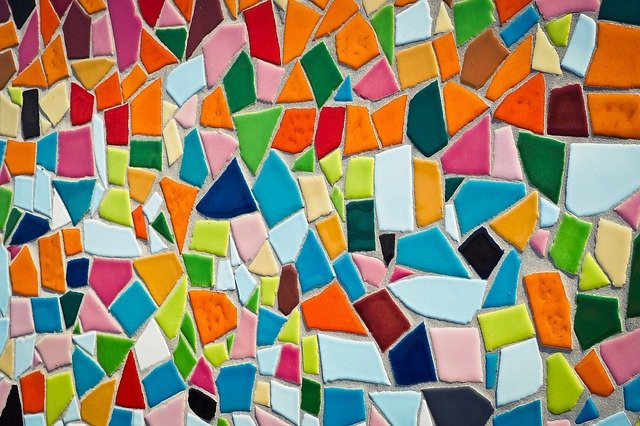
\includegraphics[scale=1.3]{pics/mosaic.jpg}}
		\caption{Mosaikbild (www.pixabay.com,\\ Fotograf: Michael Gaida)}
	\end{subfigure}\hfill
	\begin{subfigure}[t]{0.49\textwidth}
		\centering
		\boxed{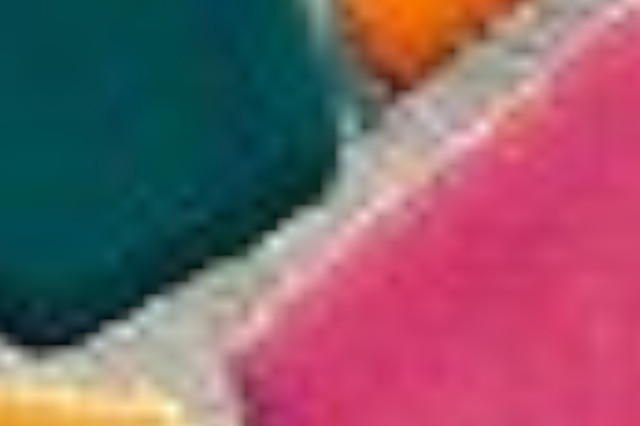
\includegraphics[scale=1.3]{pics/mosaic-zoom-20.jpg}}
		\caption{Mosaikbild bei 20-facher Vergrößerung}
	\end{subfigure}
	\caption{Bildskalierung unter Anwendung bilinearer Interpolation}
	\label{fig:MosaicBilinear}
\end{figure}
\noindent Wie zu erkennen, führt die lineare Interpolation dazu, das Kanten sehr unscharf werden und neue Farbverläufe entstehen. Im Bereich der Materialstrukturanalyse, wie später in Kapitel \ref{sec:Problemstellung} auf Seite \pageref{sec:Problemstellung} noch gezeigt wird, kann das (auch bei wesentlich kleineren Skalierungsfaktoren) zu sehr unerwünschten Einflüssen führen und Messergebnisse verfälschen.
\\\\
\noindent Abgesehen von diesen sehr einfachen Beispiel der bilinearen Interpolation gibt es jedoch auch noch einige weitere Interpolationsverfahren, bei denen die Modelle zur Approximation der fehlenden Bildinformationen auf wesentlich komplexere Art und Weise berechnet werden. Im Rahmen dieser Arbeit, kommen die folgenden zum Einsatz:
\begin{minipage}[t]{0.5\linewidth}\vspace{0pt}
	\begin{itemize}
		\item Nächster Nachbar
		\item Nächster Nachbar Exakt
		\item Linear
		\item Linear Exakt
	\end{itemize}
\end{minipage}
\begin{minipage}[t]{0.49\linewidth}\vspace{0pt}
	\begin{itemize}
		\item Kubisch
		\item Flächen-basiert
		\item Lanczos
	\end{itemize}
\end{minipage}
\\\\
\noindent Je komplexer die Algorithmen, umso genauer arbeiten sie natürlich, aber umso größer ist die Laufzeitkomplexität. Es hängt also vom konkreten Anwendungsfall ab, welcher Algorithmus zu bevorzugen ist.
\\\\
\noindent In den Kapiteln \ref{ch:Konzept} (ab Seite \pageref{ch:Konzept}) und \ref{ch:Umsetzung} (ab Seite \pageref{ch:Umsetzung}) wird das Thema wieder eine bedeutende Rolle spielen wenn es darum geht, all die benötigten Bilder mit unterschiedlichen Ausgangskalibrierungen zu erzeugen und auszuwerten, um letztlich die zentrale mit dieser Arbeit verbundenen Fragestellung beantworten zu können.

\section{Statistische Versuchsplanung}
\label{sec:StatVersPlanung}
Statistische Versuchsplanung wird häufig in der Industrie eingesetzt, um Prozesse zu optimieren. Folgende Gründe können dafür ausschlaggebend sein \cite{kleppmann_2020}:

\begin{itemize}
	\item Der Funktionsumfang der Produkte muss erhöht werden, um die Anforderungen der Kunden immer besser erfüllen zu können.
	\item Die Kosten müssen gesenkt werden, z.B. durch geringere Materialkosten oder höhere
	Ausbeute.
	\item Die Entwicklungszeit neuer Produkte und ihre Durchlaufzeit in der Fertigung müssen
	immer weiter verkürzt werden.
\end{itemize}

\noindent Diese Verbesserungen können nicht allein durch Analyse von Daten aus der Fertigung und kritisches Nachdenken erreicht werden. Dazu sind die Zusammenhänge in Entwicklung, Fertigung und Qualitätsmanagement zu kompliziert und vielschichtig. Um den Einfluss von Designänderungen auf die Eigenschaften eines neuen Produktes oder den Einfluss von Änderungen von Prozessparametern auf das Prozessergebnis zu bestimmen,
sind gezielte Versuche notwendig \cite{kleppmann_2020}.
\\\\
\noindent Diese werden mit dem Ziel durchgeführt, die komplexen Ursache-/Wirkungszusammenhänge zwischen einer oder mehrerer Stör-/ Steuergrößen und verschiedener Zielgrößen untersuchen und verstehen zu können. Es geht also darum sichtbar zumachen, welche Auswirkungen die Veränderung der Einflussgrößen auf ein bestimmtes Ergebnis haben. Dadurch wird eine gezielte Ergebnisbeeinflussung ermöglicht. Das Verhältnis zwischen Eingabe und Ausgabe (Ergebnis/Zielgröße) wird auch als Prozess bezeichnet. Zur Veranschaulichung soll die nachstehende Abbildung \ref{fig:ProzessDoe} dienen.

\begin{figure}[H]
	\centering
	\begin{tikzpicture}[x=0.75pt,y=0.75pt,yscale=-1,xscale=1, scale=1.0, every node/.style={scale=1.0}]
		%uncomment if require: \path (0,222); %set diagram left start at 0, and has height of 222
		
		%Shape: Rectangle [id:dp9587460691430016] 
		\draw  [color={rgb, 255:red, 74; green, 74; blue, 74 }  ,draw opacity=1 ][fill={rgb, 255:red, 255; green, 255; blue, 255 }  ,fill opacity=1 ] (80,60) -- (564,60) -- (564,280) -- (80,280) -- cycle ;
		%Shape: Rectangle [id:dp8844267253059725] 
		\draw  [color={rgb, 255:red, 248; green, 231; blue, 28 }  ,draw opacity=1 ][fill={rgb, 255:red, 248; green, 231; blue, 28 }  ,fill opacity=1 ] (220,172) -- (420,172) -- (420,252) -- (220,252) -- cycle ;
		%Straight Lines [id:da8411829174990819] 
		\draw [color={rgb, 255:red, 126; green, 211; blue, 33 }  ,draw opacity=1 ][line width=4.5]    (273,128) -- (273,160) ;
		\draw [shift={(273,168)}, rotate = 270] [fill={rgb, 255:red, 126; green, 211; blue, 33 }  ,fill opacity=1 ][line width=0.08]  [draw opacity=0] (24.11,-11.58) -- (0,0) -- (24.11,11.58) -- cycle    ;
		%Straight Lines [id:da7471836258073241] 
		\draw [color={rgb, 255:red, 126; green, 211; blue, 33 }  ,draw opacity=1 ][line width=4.5]    (374,128) -- (374,160) ;
		\draw [shift={(374,168)}, rotate = 270] [fill={rgb, 255:red, 126; green, 211; blue, 33 }  ,fill opacity=1 ][line width=0.08]  [draw opacity=0] (24.11,-11.58) -- (0,0) -- (24.11,11.58) -- cycle    ;
		%Notched Right Arrow [id:dp19574990057369157] 
		\draw  [color={rgb, 255:red, 126; green, 211; blue, 33 }  ,draw opacity=1 ][fill={rgb, 255:red, 126; green, 211; blue, 33 }  ,fill opacity=1 ] (432,195.75) -- (502.2,195.75) -- (502.2,181) -- (549,210.5) -- (502.2,240) -- (502.2,225.25) -- (432,225.25) -- (446.75,210.5) -- cycle ;
		%Notched Right Arrow [id:dp2222830717379538] 
		\draw  [color={rgb, 255:red, 126; green, 211; blue, 33 }  ,draw opacity=1 ][fill={rgb, 255:red, 126; green, 211; blue, 33 }  ,fill opacity=1 ] (93,195.75) -- (163.2,195.75) -- (163.2,181) -- (210,210.5) -- (163.2,240) -- (163.2,225.25) -- (93,225.25) -- (107.75,210.5) -- cycle ;
		
		% Text Node
		\draw (243.06,198.75) node [anchor=north west][inner sep=0.75pt]  [color={rgb, 255:red, 74; green, 74; blue, 74 }  ,opacity=1 ,rotate=-0.19] [align=left] {\begin{minipage}[lt]{111.75pt}\setlength\topsep{0pt}
				\begin{center}
					\textbf{{\large PROZESS}}\\{\scriptsize \textbf{\textit{Ursache-/Wirgungsbez.}}}
				\end{center}
				
		\end{minipage}};
		% Text Node
		\draw (322,76) node [anchor=north west][inner sep=0.75pt]  [color={rgb, 255:red, 74; green, 74; blue, 74 }  ,opacity=1 ] [align=left] {\begin{minipage}[lt]{72.94pt}\setlength\topsep{0pt}
				\begin{center}
					\textbf{Störgrößen}\\{\scriptsize \textbf{\textit{(nicht beeinflussbar)}}}\\
				\end{center}
				
		\end{minipage}};
		% Text Node
		\draw (222,76) node [anchor=north west][inner sep=0.75pt]  [color={rgb, 255:red, 74; green, 74; blue, 74 }  ,opacity=1 ] [align=left] {\begin{minipage}[lt]{69.03pt}\setlength\topsep{0pt}
				\begin{center}
					\textbf{Steuergrößen}\\{\scriptsize \textbf{\textit{(beinfussbar)}}}
				\end{center}
				
		\end{minipage}};
		% Text Node
		\draw (452,201) node [anchor=north west][inner sep=0.75pt]  [font=\scriptsize,color={rgb, 255:red, 74; green, 74; blue, 74 }  ,opacity=1 ] [align=left] {\textbf{AUSGABE/}\\\textbf{ERGEBNIS}};
		% Text Node
		\draw (113,206) node [anchor=north west][inner sep=0.75pt]  [font=\scriptsize,color={rgb, 255:red, 74; green, 74; blue, 74 }  ,opacity=1 ] [align=left] {\textbf{EINGABE}};
	\end{tikzpicture}
	\caption{Prozessmodell zur statistischen Versuchsplanung}
	\label{fig:ProzessDoe}
\end{figure}

\noindent Die Abbildung zeigt einen beliebigen Prozess der dadurch gekennzeichnet ist, dass eine Eingabe unter dem Einfluss von verschiedenen Steuer- und Störgrößen ein bestimmtes erzeugt wird. Außerdem zu erkennen ist eine Unterteilung der Einflussgrößen in Steuer- und Störgrößen. Das geschieht deshalb, weil es Einflussfaktoren geben kann, die während des Prozessverlaufs nicht beeinflusst werden können. \textcolor{red}{Ein Beispiel dafür wäre etwa die Außentemperatur in einer Fabrikhalle, die negative Einflüsse auf die Präzisionsgenauigkeit eines Industrieroboters haben kann, da sich das Material, aus dem der Roboter gefertigt ist (meistens Stahl) bei hohen Temperaturen (also zur Sommerzeit) ausdehnt. Im Rahmen einer Systemanalyse ist dieser Faktor zwar von hoher Relevanz, kann aber in der Praxis oftmals, wenn überhaupt, nur sehr begrenzt beeinflusst werden, also eine sog. Störgröße. Die Steuergrößen wären hier dann z.B. die einzelnen Einstellparameter (Gelenkwinkelstellungen des Roboterarmes) innerhalb der kinematischen Kette des Roboters, welche gezielt beeinflussbar sind und in direktem Zusammenhang mit der Präzisionsgenauigkeit stehen.
\\\\
Um nun die richtigen Einstellungen in Abhängigkeit von der Außentemperatur zu finden wäre es natürlich denkbar und möglich, immer nur einen Parameter bei unterschiedlichen Temperaturen zu verändern und so die optimale Einstellung bezogen auf die Genauigkeit für jeden der einzelnen Parameter zu finden. Diese Vorgehensweise führt aber deshalb oft nicht zum optimalen Ergebnis, da hierbei nur jeder einzelne Parameter in Abhängigkeit von der Temperatur untersucht wurde, aber nicht die Wechselbeziehungen zwischen den Stör- und den Steuergrößen untereinander.}
\\\\
\noindent Was in diesem Modell also noch fehlt, um zu einer ganzheitlichen Analyse zu gelangen, ist die Einbeziehung dieser Wechselwirkungen  in das Modell. Denn nur durch die Betrachtung der Gesamtdynamik eines Systems ist es möglich, ein globales Optimum zu finden. Bezogen auf das o.g. Beispiel mit dem Industrieroboter können auf diese Weise Erkenntnisse darüber gewonnen werden, wie genau sich die Außentemperatur auf verschiedene Parameter der kinematischen Kette des Roboters (unter Einbeziehung der Wechselwirkungen zwischen den Steuergrößen untereinander) auswirkt und wie diese in Abhängigkeit von der Außentemperatur angepasst werden müssten, um das Ergebnis (hier: Präzisionsgenauigkeit) in die gewünschte Richtung zu beeinflussen. Im Rahmen einer statistischen Versuchsplanung wir genau dieses Ziel verfolgt, wobei diese Vorgehensweise auf beliebige Systeme angewendet werden kann, bei denen es darum geht, eine oder mehrere Zielgrößen in Abhängigkeit von mehreren beeinflussenden Faktoren zu optimieren.
\\\\
Nach \cite{schiefer_2018} kann zwischen den in nachstehender Abbildung \ref{fig:Versuchsplaene} dargestellten Versuchsplänen unterschieden werden:

\begin{figure}[H]
	\centering
	\begin{tikzpicture}[x=0.75pt,y=0.75pt,yscale=-1,xscale=1, scale=0.55, every node/.style={scale=0.55}]
		%uncomment if require: \path (0,222); %set diagram left start at 0, and has height of 222
		
		%Shape: Rectangle [id:dp5078039108352421] 
		\draw  [color={rgb, 255:red, 74; green, 74; blue, 74 }  ,draw opacity=1 ][line width=1.5]  (85,52) -- (558,52) -- (558,450) -- (85,450) -- cycle ;
		
		% Text Node
		\draw (265,239) node [anchor=north west][inner sep=0.75pt]  [color={rgb, 255:red, 74; green, 74; blue, 74 }  ,opacity=1 ] [align=left] {{\Large \textbf{\textcolor[rgb]{0.29,0.29,0.29}{Versuchspläne}}}};
		% Text Node
		\draw (124,72) node [anchor=north west][inner sep=0.75pt]   [align=left] {\begin{minipage}[lt]{142.35pt}\setlength\topsep{0pt}
				\begin{center}
					\textbf{\textcolor[rgb]{0.29,0.56,0.89}{vollständig faktorieller }}\\\textbf{\textcolor[rgb]{0.29,0.56,0.89}{Versuchsplan}}\\{\footnotesize \textcolor[rgb]{0.29,0.29,0.29}{Dabei werden die Einflussfaktoren }}\\{\footnotesize \textcolor[rgb]{0.29,0.29,0.29}{in ihren Stufen vollständig kombiniert und gleichzeitig variiert.}}
				\end{center}
				
		\end{minipage}};
		% Text Node
		\draw (348,332) node [anchor=north west][inner sep=0.75pt]   [align=left] {\begin{minipage}[lt]{142.63pt}\setlength\topsep{0pt}
				\begin{center}
					\textbf{\textcolor[rgb]{0.97,0.91,0.11}{teilfaktorieller Versuchsplan}}\\{\footnotesize \textcolor[rgb]{0.29,0.29,0.29}{Ist bei der Aufgabenstellung nicht die }}\\{\footnotesize \textcolor[rgb]{0.29,0.29,0.29}{vollständige Wechselwirkung der }}\\{\footnotesize \textcolor[rgb]{0.29,0.29,0.29}{Einflussgrößen auf die Zielgröße }}\\{\footnotesize \textcolor[rgb]{0.29,0.29,0.29}{von Interesse, lässt sich der }}\\{\footnotesize \textcolor[rgb]{0.29,0.29,0.29}{Versuchsplan reduzieren.}}
				\end{center}
				
		\end{minipage}};
		% Text Node
		\draw (343,88) node [anchor=north west][inner sep=0.75pt]   [align=left] {\begin{minipage}[lt]{138.17pt}\setlength\topsep{0pt}
				\begin{center}
					\textbf{\textcolor[rgb]{0.49,0.83,0.13}{faktorieller Versuchsplan }}\\\textbf{\textcolor[rgb]{0.49,0.83,0.13}{mit Zentralpunkt}}\\{\footnotesize \textcolor[rgb]{0.29,0.29,0.29}{Wird verwendet, um zu überprüfen }}\\{\footnotesize \textcolor[rgb]{0.29,0.29,0.29}{ob Nichtlinearitäten vorliegen.}}
				\end{center}
				
		\end{minipage}};
		% Text Node
		\draw (109,330) node [anchor=north west][inner sep=0.75pt]   [align=left] {\begin{minipage}[lt]{148.78pt}\setlength\topsep{0pt}
				\begin{center}
					\textbf{\textcolor[rgb]{0.74,0.06,0.88}{lateinische Quadrate}}\\{\footnotesize \textcolor[rgb]{0.29,0.29,0.29}{Nur dann sinnvoll, wenn gesichert ist, }}\\{\footnotesize \textcolor[rgb]{0.29,0.29,0.29}{dass Wechselwirkungen zwischen den }}\\{\footnotesize \textcolor[rgb]{0.29,0.29,0.29}{Einflussgrößen keine Rolle spielen oder }}\\{\footnotesize \textcolor[rgb]{0.29,0.29,0.29}{vernachlässigt \ werden können.}}
				\end{center}
				
		\end{minipage}};
		% Connection
		\draw [color={rgb, 255:red, 189; green, 16; blue, 224 }  ,draw opacity=1 ][line width=3]    (317.03,267) -- (269.03,321.5) ;
		\draw [shift={(265.06,326)}, rotate = 311.37] [fill={rgb, 255:red, 189; green, 16; blue, 224 }  ,fill opacity=1 ][line width=0.08]  [draw opacity=0] (16.97,-8.15) -- (0,0) -- (16.97,8.15) -- cycle    ;
		% Connection
		\draw [color={rgb, 255:red, 248; green, 231; blue, 28 }  ,draw opacity=1 ][line width=3]    (346.14,267) -- (393.03,323.39) ;
		\draw [shift={(396.86,328)}, rotate = 230.25] [fill={rgb, 255:red, 248; green, 231; blue, 28 }  ,fill opacity=1 ][line width=0.08]  [draw opacity=0] (16.97,-8.15) -- (0,0) -- (16.97,8.15) -- cycle    ;
		% Connection
		\draw [color={rgb, 255:red, 74; green, 144; blue, 226 }  ,draw opacity=1 ][line width=3]    (318.32,233) -- (272.2,175.67) ;
		\draw [shift={(268.44,171)}, rotate = 411.18] [fill={rgb, 255:red, 74; green, 144; blue, 226 }  ,fill opacity=1 ][line width=0.08]  [draw opacity=0] (16.97,-8.15) -- (0,0) -- (16.97,8.15) -- cycle    ;
		% Connection
		\draw [color={rgb, 255:red, 126; green, 211; blue, 33 }  ,draw opacity=1 ][line width=3]    (346.77,233) -- (395.84,176.53) ;
		\draw [shift={(399.77,172)}, rotate = 490.99] [fill={rgb, 255:red, 126; green, 211; blue, 33 }  ,fill opacity=1 ][line width=0.08]  [draw opacity=0] (16.97,-8.15) -- (0,0) -- (16.97,8.15) -- cycle    ;
	\end{tikzpicture}
	\caption{Arten von Versuchsplänen}
	\label{fig:Versuchsplaene}
\end{figure}

\noindent Welcher Versuchsplan der Richtige ist, hängt von der jeweiligen Aufgabenstellung ab. Da in der vorliegenden Arbeit eine statistische Auswertung anhand eines \textbf{vollständig faktoriellen Versuchsplans} erfolgt, beschränken sich die weiteren Ausführungen in diesem Kapitel auf dessen detaillierter Beschreibung.
\\\\
\noindent Von elementarer Bedeutung ist es zu wissen, wie viele \textbf{Einflussfaktoren (k)} im Rahmen einer Untersuchung vorliegen und im Modell entsprechend zu berücksichtigen sind und welche \textbf{Variationsstufen (n)} innerhalb eines Faktors möglich sind. Die Anzahl der durchzuführenden Versuche (z) kann dann allgemein wie folgt berechnet werden:
\\\\
\begin{equation}
	\mathbf{z = n^k}
\end{equation}
\\\\
\noindent Wird bspw. ein System mit 3 Einflussfaktoren untersucht, die jeweils in 2 Stufen $(+/-)$ variiert werden können, müssen bei einem vollständig faktoriellen Versuchsplan also $3^2 = 8$ Versuche durchgeführt werden. Der sich daraus ergebende Plan ist in folgender Tabelle \ref{tab:Versuchsplan} dargestellt.

\begin{minipage}[t]{0.4\linewidth}\vspace{0pt}
	\begin{table}[H]
		\centering
		\caption{Versuchsplan mit 3 Einflussfaktoren und jeweils 2 Faktorstufenkombinationen}
		\label{tab:Versuchsplan}
		\begin{tabular}{@{}cccc@{}}
			\toprule[3pt]
			\multicolumn{1}{l}{\textbf{\begin{tabular}[c]{@{}l@{}}Anzahl\\ Versuche\end{tabular}}} & \multicolumn{3}{l}{\textbf{\begin{tabular}[c]{@{}l@{}}Faktorstufen-\\ kombinationen\end{tabular}}} \\ \midrule[3pt]
			\multicolumn{1}{l}{\textbf{}}                                                          & \textbf{A}                      & \textbf{B}                      & \textbf{C}                     \\ \midrule
			\textbf{1}                                                                             & -                               & -                               & -                              \\ \midrule
			\textbf{2}                                                                             & -                               & -                               & +                              \\ \midrule
			\textbf{3}                                                                             & -                               & +                               & -                              \\ \midrule
			\textbf{4}                                                                             & -                               & +                               & +                              \\ \midrule
			\textbf{5}                                                                             & +                               & -                               & -                              \\ \midrule
			\textbf{6}                                                                             & +                               & -                               & +                              \\ \midrule
			\textbf{7}                                                                             & +                               & +                               & -                              \\ \midrule
			\textbf{8}                                                                             & +                               & +                               & +                              \\ \bottomrule[3pt]
		\end{tabular}
	\end{table}
\end{minipage}
\begin{minipage}[t]{0.59\linewidth}\vspace{0pt}
	\begin{figure}[H]
		\centering
		\medskip\medskip\medskip\medskip\medskip\medskip\medskip\medskip\smallskip
		\begin{tikzpicture}[x=0.75pt,y=0.75pt,yscale=-1,xscale=1, scale=0.6, every node/.style={scale=0.6}]
			%uncomment if require: \path (0,222); %set diagram left start at 0, and has height of 222
			
			%Straight Lines [id:da017743038240972897] 
			\draw [color={rgb, 255:red, 126; green, 211; blue, 33 }  ,draw opacity=1 ][line width=2.25]    (320,389) -- (320,409) ;
			%Straight Lines [id:da5646155797639212] 
			\draw [color={rgb, 255:red, 126; green, 211; blue, 33 }  ,draw opacity=1 ][line width=2.25]    (482,350) -- (499.8,350) ;
			%Straight Lines [id:da5139851724668463] 
			\draw [color={rgb, 255:red, 126; green, 211; blue, 33 }  ,draw opacity=1 ][line width=2.25]    (432,279) -- (449.8,279) ;
			
			% Text Node
			\draw (314,419) node [anchor=north west][inner sep=0.75pt]   [align=left] {\textbf{\textcolor[rgb]{0.49,0.83,0.13}{A}}};
			% Text Node
			\draw (520,360) node [anchor=north west][inner sep=0.75pt]   [align=left] {\textbf{\textcolor[rgb]{0.49,0.83,0.13}{B}}};
			% Text Node
			\draw (464,270) node [anchor=north west][inner sep=0.75pt]   [align=left] {\textbf{\textcolor[rgb]{0.49,0.83,0.13}{C}}};
			% Text Node
			\draw (174,385) node [anchor=north west][inner sep=0.75pt]   [align=left] {\begin{minipage}[lt]{38.5pt}\setlength\topsep{0pt}
					\begin{center}
						\textbf{\textcolor[rgb]{0.29,0.56,0.89}{1}}\\\textbf{\textcolor[rgb]{0.29,0.56,0.89}{(- - -)}}
					\end{center}
					
			\end{minipage}};
			% Text Node
			\draw (174,145) node [anchor=north west][inner sep=0.75pt]   [align=left] {\begin{minipage}[lt]{38.5pt}\setlength\topsep{0pt}
					\begin{center}
						\textbf{\textcolor[rgb]{0.29,0.56,0.89}{2}}\\\textbf{\textcolor[rgb]{0.29,0.56,0.89}{(- - +)}}
					\end{center}
					
			\end{minipage}};
			% Text Node
			\draw (274,288) node [anchor=north west][inner sep=0.75pt]   [align=left] {\begin{minipage}[lt]{38.5pt}\setlength\topsep{0pt}
					\begin{center}
						\textbf{\textcolor[rgb]{0.29,0.56,0.89}{3}}\\\textbf{\textcolor[rgb]{0.29,0.56,0.89}{(- + -)}}
					\end{center}
					
			\end{minipage}};
			% Text Node
			\draw (360,411) node [anchor=north west][inner sep=0.75pt]   [align=left] {\textbf{\textcolor[rgb]{0.49,0.83,0.13}{+}}};
			% Text Node
			\draw (266,414) node [anchor=north west][inner sep=0.75pt]   [align=left] {\begin{minipage}[lt]{8.67pt}\setlength\topsep{0pt}
					\begin{center}
						\textbf{\textcolor[rgb]{0.49,0.83,0.13}{-}}
					\end{center}
					
			\end{minipage}};
			% Text Node
			\draw (495,370) node [anchor=north west][inner sep=0.75pt]   [align=left] {\begin{minipage}[lt]{8.67pt}\setlength\topsep{0pt}
					\begin{center}
						\textbf{\textcolor[rgb]{0.49,0.83,0.13}{-}}
					\end{center}
					
			\end{minipage}};
			% Text Node
			\draw (512,342) node [anchor=north west][inner sep=0.75pt]   [align=left] {\textbf{\textcolor[rgb]{0.49,0.83,0.13}{+}}};
			% Text Node
			\draw (450,231) node [anchor=north west][inner sep=0.75pt]   [align=left] {\textbf{\textcolor[rgb]{0.49,0.83,0.13}{+}}};
			% Text Node
			\draw (451,323) node [anchor=north west][inner sep=0.75pt]   [align=left] {\begin{minipage}[lt]{8.67pt}\setlength\topsep{0pt}
					\begin{center}
						\textbf{\textcolor[rgb]{0.49,0.83,0.13}{-}}
					\end{center}
					
			\end{minipage}};
			% Text Node
			\draw (274,46) node [anchor=north west][inner sep=0.75pt]   [align=left] {\begin{minipage}[lt]{38.5pt}\setlength\topsep{0pt}
					\begin{center}
						\textbf{\textcolor[rgb]{0.29,0.56,0.89}{4}}\\\textbf{\textcolor[rgb]{0.29,0.56,0.89}{(- + +)}}
					\end{center}
					
			\end{minipage}};
			% Text Node
			\draw (417,385) node [anchor=north west][inner sep=0.75pt]   [align=left] {\begin{minipage}[lt]{33.94pt}\setlength\topsep{0pt}
					\begin{center}
						\textbf{\textcolor[rgb]{0.29,0.56,0.89}{5}}\\\textbf{\textcolor[rgb]{0.29,0.56,0.89}{(+ - -)}}
					\end{center}
					
			\end{minipage}};
			% Text Node
			\draw (415,145) node [anchor=north west][inner sep=0.75pt]   [align=left] {\begin{minipage}[lt]{38.5pt}\setlength\topsep{0pt}
					\begin{center}
						\textbf{\textcolor[rgb]{0.29,0.56,0.89}{6}}\\\textbf{\textcolor[rgb]{0.29,0.56,0.89}{(+ - +})}
					\end{center}
					
			\end{minipage}};
			% Text Node
			\draw (515,288) node [anchor=north west][inner sep=0.75pt]   [align=left] {\begin{minipage}[lt]{38.5pt}\setlength\topsep{0pt}
					\begin{center}
						\textbf{\textcolor[rgb]{0.29,0.56,0.89}{7}}\\\textbf{\textcolor[rgb]{0.29,0.56,0.89}{(+ + -)}}
					\end{center}
					
			\end{minipage}};
			% Text Node
			\draw (509,48) node [anchor=north west][inner sep=0.75pt]   [align=left] {\begin{minipage}[lt]{44.5pt}\setlength\topsep{0pt}
					\begin{center}
						\textbf{\textcolor[rgb]{0.29,0.56,0.89}{8}}\\\textbf{\textcolor[rgb]{0.29,0.56,0.89}{(+ + +)}}
					\end{center}
					
			\end{minipage}};
			% Text Node
			\draw  [color={rgb, 255:red, 74; green, 144; blue, 226 }  ,draw opacity=1 ][line width=1.5]   (382, 222.5) circle [x radius= 76.37, y radius= 14.85]   ;
			\draw (331,217) node [anchor=north west][inner sep=0.75pt]   [align=left] {\textbf{\textcolor[rgb]{0.29,0.56,0.89}{Versuchsraum}}};
			% Connection
			\draw [line width=1.5]    (464.87,375.38) -- (514.93,326.79) ;
			\draw [shift={(517.8,324)}, rotate = 495.86] [fill={rgb, 255:red, 0; green, 0; blue, 0 }  ][line width=0.08]  [draw opacity=0] (11.61,-5.58) -- (0,0) -- (11.61,5.58) -- cycle    ;
			\draw [shift={(462,378.16)}, rotate = 315.86] [fill={rgb, 255:red, 0; green, 0; blue, 0 }  ][line width=0.08]  [draw opacity=0] (11.61,-5.58) -- (0,0) -- (11.61,5.58) -- cycle    ;
			% Connection
			\draw [line width=1.5]    (541.39,274) -- (540.61,88) ;
			\draw [shift={(540.6,84)}, rotate = 449.76] [fill={rgb, 255:red, 0; green, 0; blue, 0 }  ][line width=0.08]  [draw opacity=0] (11.61,-5.58) -- (0,0) -- (11.61,5.58) -- cycle    ;
			\draw [shift={(541.4,278)}, rotate = 269.76] [fill={rgb, 255:red, 0; green, 0; blue, 0 }  ][line width=0.08]  [draw opacity=0] (11.61,-5.58) -- (0,0) -- (11.61,5.58) -- cycle    ;
			% Connection
			\draw [line width=1.5]    (439.72,373) -- (441.28,186) ;
			\draw [shift={(441.31,182)}, rotate = 450.48] [fill={rgb, 255:red, 0; green, 0; blue, 0 }  ][line width=0.08]  [draw opacity=0] (11.61,-5.58) -- (0,0) -- (11.61,5.58) -- cycle    ;
			\draw [shift={(439.69,377)}, rotate = 270.48] [fill={rgb, 255:red, 0; green, 0; blue, 0 }  ][line width=0.08]  [draw opacity=0] (11.61,-5.58) -- (0,0) -- (11.61,5.58) -- cycle    ;
			% Connection
			\draw [line width=1.5]    (225,399.1) -- (413,399.89) ;
			\draw [shift={(417,399.91)}, rotate = 180.24] [fill={rgb, 255:red, 0; green, 0; blue, 0 }  ][line width=0.08]  [draw opacity=0] (11.61,-5.58) -- (0,0) -- (11.61,5.58) -- cycle    ;
			\draw [shift={(221,399.09)}, rotate = 0.24] [fill={rgb, 255:red, 0; green, 0; blue, 0 }  ][line width=0.08]  [draw opacity=0] (11.61,-5.58) -- (0,0) -- (11.61,5.58) -- cycle    ;
			% Connection
			\draw [line width=1.5]    (200.61,372) -- (201.39,186) ;
			\draw [shift={(201.4,182)}, rotate = 450.24] [fill={rgb, 255:red, 0; green, 0; blue, 0 }  ][line width=0.08]  [draw opacity=0] (11.61,-5.58) -- (0,0) -- (11.61,5.58) -- cycle    ;
			\draw [shift={(200.6,376)}, rotate = 270.24] [fill={rgb, 255:red, 0; green, 0; blue, 0 }  ][line width=0.08]  [draw opacity=0] (11.61,-5.58) -- (0,0) -- (11.61,5.58) -- cycle    ;
			% Connection
			\draw [line width=1.5]    (228,159) -- (413,159) ;
			\draw [shift={(417,159)}, rotate = 180] [fill={rgb, 255:red, 0; green, 0; blue, 0 }  ][line width=0.08]  [draw opacity=0] (11.61,-5.58) -- (0,0) -- (11.61,5.58) -- cycle    ;
			\draw [shift={(224,159)}, rotate = 0] [fill={rgb, 255:red, 0; green, 0; blue, 0 }  ][line width=0.08]  [draw opacity=0] (11.61,-5.58) -- (0,0) -- (11.61,5.58) -- cycle    ;
			% Connection
			\draw [line width=1.5]    (226.87,134.38) -- (275.93,86.79) ;
			\draw [shift={(278.8,84)}, rotate = 495.86] [fill={rgb, 255:red, 0; green, 0; blue, 0 }  ][line width=0.08]  [draw opacity=0] (11.61,-5.58) -- (0,0) -- (11.61,5.58) -- cycle    ;
			\draw [shift={(224,137.17)}, rotate = 315.86] [fill={rgb, 255:red, 0; green, 0; blue, 0 }  ][line width=0.08]  [draw opacity=0] (11.61,-5.58) -- (0,0) -- (11.61,5.58) -- cycle    ;
			% Connection
			\draw [line width=1.5]    (467.58,133.19) -- (514.42,86.81) ;
			\draw [shift={(517.27,84)}, rotate = 495.29] [fill={rgb, 255:red, 0; green, 0; blue, 0 }  ][line width=0.08]  [draw opacity=0] (11.61,-5.58) -- (0,0) -- (11.61,5.58) -- cycle    ;
			\draw [shift={(464.73,136)}, rotate = 315.29] [fill={rgb, 255:red, 0; green, 0; blue, 0 }  ][line width=0.08]  [draw opacity=0] (11.61,-5.58) -- (0,0) -- (11.61,5.58) -- cycle    ;
			% Connection
			\draw [line width=1.5]    (331,61) -- (510,61) ;
			\draw [shift={(514,61)}, rotate = 180] [fill={rgb, 255:red, 0; green, 0; blue, 0 }  ][line width=0.08]  [draw opacity=0] (11.61,-5.58) -- (0,0) -- (11.61,5.58) -- cycle    ;
			\draw [shift={(327,61)}, rotate = 0] [fill={rgb, 255:red, 0; green, 0; blue, 0 }  ][line width=0.08]  [draw opacity=0] (11.61,-5.58) -- (0,0) -- (11.61,5.58) -- cycle    ;
			% Connection
			\draw [line width=1.5]  [dash pattern={on 5.63pt off 4.5pt}]  (302.27,88) -- (300.73,273) ;
			\draw [shift={(300.69,277)}, rotate = 270.48] [fill={rgb, 255:red, 0; green, 0; blue, 0 }  ][line width=0.08]  [draw opacity=0] (11.61,-5.58) -- (0,0) -- (11.61,5.58) -- cycle    ;
			\draw [shift={(302.31,84)}, rotate = 90.48] [fill={rgb, 255:red, 0; green, 0; blue, 0 }  ][line width=0.08]  [draw opacity=0] (11.61,-5.58) -- (0,0) -- (11.61,5.58) -- cycle    ;
			% Connection
			\draw [line width=1.5]  [dash pattern={on 5.63pt off 4.5pt}]  (327,300.11) -- (513,300.88) ;
			\draw [shift={(517,300.9)}, rotate = 180.24] [fill={rgb, 255:red, 0; green, 0; blue, 0 }  ][line width=0.08]  [draw opacity=0] (11.61,-5.58) -- (0,0) -- (11.61,5.58) -- cycle    ;
			\draw [shift={(323,300.09)}, rotate = 0.24] [fill={rgb, 255:red, 0; green, 0; blue, 0 }  ][line width=0.08]  [draw opacity=0] (11.61,-5.58) -- (0,0) -- (11.61,5.58) -- cycle    ;
			% Connection
			\draw [line width=1.5]  [dash pattern={on 5.63pt off 4.5pt}]  (223.84,375.89) -- (275.16,325.09) ;
			\draw [shift={(278,322.27)}, rotate = 495.29] [fill={rgb, 255:red, 0; green, 0; blue, 0 }  ][line width=0.08]  [draw opacity=0] (11.61,-5.58) -- (0,0) -- (11.61,5.58) -- cycle    ;
			\draw [shift={(221,378.71)}, rotate = 315.29] [fill={rgb, 255:red, 0; green, 0; blue, 0 }  ][line width=0.08]  [draw opacity=0] (11.61,-5.58) -- (0,0) -- (11.61,5.58) -- cycle    ;
			
		\end{tikzpicture}
		\caption{Darstellung des Versuchsraumes aus 3 Einflussfaktoren und Faktorstufenkombinationen $(+/-)$}
		\label{fig:Versuchsplan}
	\end{figure}
\end{minipage}
\\\\\\
\noindent Die sich ergebenden Faktorstufenkombinationen aus der Tabelle beschreiben, bei 3 Einflussfaktoren einen 3-Dimensionalen Raum, wie in Abbildung \ref{fig:Versuchsplan} dargestellt. Dieser wird jeweils durch die minimalen und maximalen Ausprägungen begrenzt und beschreiben den sog. Versuchsraum, der alle möglichen Wirkungen enthält. 
\\\\
\noindent Der Vorteil von vollständig faktoriellen Versuchsplänen ist der, dass wirklich alle möglichen Faktorausprägungen und Wirkungen in der Analyse berücksichtigt werden, und somit der Erkenntnisgewinn am größten ist. Allerdings können diese Pläne sehr schnell auch extrem groß werden, wodurch die Durchführung in der Praxis oftmals aus Kosten- und/oder Zeitgründen unmöglich ist. In solchen  Fällen kann dann auf die Verwendung von teilfaktoriellen Plänen ausgewichen werden.
\\\\
\noindent In Kapitel \ref{ch:Konzept} auf Seite \pageref{ch:Konzept} wird das hier beschriebene Modell eines vollständig faktoriellen Versuchsplanes wieder aufgegriffen und dahingehend erweitert, das eine Anwendung zur Untersuchung der im Rahmen dieser Arbeit zu untersuchenden Fragestellung möglich wird. In Kapitel \ref{ch:Evaluation} auf Seite \pageref{ch:Evaluation} werden die Untersuchungsergebnisse dann anhand dieses Modells schließlich ausgewertet und interpretiert.

\section{Überblick über die Skriptsprache AutoIt}
\label{sec:UeberblickAutoIt}

Im Rahmen dieser Arbeit wird AutoIt einerseits dazu genutzt, um die zur Evaluation der Wirkungsweise von unterschiedlichen Interpolationsalgorithmen benötigten Daten zu generieren. Dazu ist es nötig, tausende von Lamellenguss-Messungen mit der Software AMGuss durchzuführen. Dies wäre ohne Automatisierung mit einem nicht vertretbaren Zeitaufwand verbunden. Die automatische Durchführung der Messungen mit AutoIt funktioniert dagegen nach einigen Tests sehr gut und der Zeitaufwand lässt sich somit auf etwa 20 Sekunden pro Messung reduzieren.
\\\\
\noindent Gemäß offizieller Dokumentation \cite{AutoItDocs} lässt sich AutoIT wie folgt beschreiben:
\\\\
\noindent Es handelt sich dabei um eine BASIC-ähnliche Skriptsprache, die zur Automatisierung von Windows-Benutzeroberflächen entwickelt wurde. Es verwendet eine Kombination aus simulierten Tastenanschlägen, Mausbewegungen sowie Fenster- und Steuerungsmanipulationen, um Aufgaben auf eine Weise zu automatisieren, die mit anderen Sprachen (z.B. VBScript und SendKeys) nicht möglich ist.
\\\\
\noindent AutoIt wurde ursprünglich für PC-Rollout-Situationen entwickelt, um Tausende von PCs zuverlässig zu automatisieren und zu konfigurieren. Im Laufe der Zeit hat es sich zu einer leistungsstarken Sprache entwickelt, die komplexe Ausdrücke, Benutzerfunktionen, Schleifen und alles andere unterstützt, was erfahrene Skripter erwarten würden. 
\\\\
\textbf{Die wichtigsten Eigenschaften kurz zusammengefasst:}
\begin{itemize}
	\item Einfach zu erlernende BASIC-ähnliche Syntax
	\item Simulation von Tastenanschlägen und Mausbewegungen
	\item Steuerung von Fenstern und Prozessen
	\item Interaktion mit Standard-Windows-Steuerelementen
	\item Kompilierung von Skripten zu eigenen ausführbaren Dateien
	\item Erstellung grafischer Benutzeroberflächen
	\item COM-Unterstützung
	\item Reguläre Ausdrücke
	\item Direkter Aufruf von Funktionen aus externen DLL's sowie von Windows-API-Funktionen
	\item etc.
\end{itemize}

\chapter{Ausgangssituation}
\label{ch:Ausgangssituation}
Ziel dieses Kapitels ist es die Ausgangssituation, also die mit dieser Arbeit verbundenen Rahmenbedingungen im Detail darzulegen, um damit die Grundlage für eine schlüssige Präsentation des Lösungskonzeptes im darauf folgenden Kapitel \ref{ch:Konzept} zu schaffen.
\\\\
Im Abschnitt \ref{sec:BestimmungMikrostrukturAMGuss} wird zunächst auf die Bedeutung des Einsatzes digitaler Bildverarbeitung zur Analyse von Gusseisen eingegangen und in diesem Zusammenhang die Software AMGuss vorgestellt. Dabei wird auf die Bedeutung eines Anordnungsklassifikators eingegangen und die Erstellung eines Solchen im Detail dargestellt (\ref{subsec: ErstellungAnordnungsklassifAMGuss}),  der vollständige Ablauf bei der Durchführung einer Messung beschrieben (\ref{subsec:LamelloGraphMesssung}) und schließlich die durch eine Auswertung erzeugten Messergebnisse einer genaueren Betrachtung unterzogen (\ref{subsec:ErgebnisseAMGuss}).
\\\\
Ergänzend dazu wird im Abschnitt \ref{subsec:Bildmaterial} auf das zur Verfügung stehende Bildmaterial eingegangen und das Kapitel schließt mit einer ausführlichen Problembeschreibung in Abschnitt \ref{sec:Problemstellung}.

\section{Einsatz digitaler Bildverarbeitung zur Analyse der Mikrostruktur von Gusseisen (AMGuss)}
\label{sec:BestimmungMikrostrukturAMGuss}
Wegen der mit rein visueller Qualitätskontrolle verbundenen Probleme, die bereits in Kapitel \ref{subsec:MethodenBestAnordnungsklassen} auf Seite \pageref{subsec:MethodenBestAnordnungsklassen} dargelegt wurden, war ein automatisch ablaufendes Analyseverfahren zur Bestimmung der Mikrostruktur von Gusseisen, erweitert um Bilddokumentation und Bildarchivierung, ein großes Anliegen in den Laboren der Eisengießereien. Dadurch sollte eines der Grundanliegen des Qualitätsmanagements erfüllt werden, nämlich die quantitative Charakterisierung des Gussvorgangs durch Bereitstellung aussagekräftiger Messparameter und Objektivierung der Messergebnisse. Aus diesem Anliegen heraus entstand bei der GFaI e.V. bereits im Jahr 2005 ein Forschungsprojekt mit der Zielsetzung, die Grundlage zur Entwicklung eines marktreifen Software-Produktes zu schaffen, mit dem sich alle geforderten Normparameter der Mikrostruktur von Gusseisen automatisch (oder zumindest halbautomatisch) bestimmen lassen. \cite{AMGuss2007}.
\\\\
Das Ergebnis dieses Forschungsprojektes ist die Software AMGuss (\textbf{A}nalyse der \textbf{M}ikrostruktur von \textbf{Guss}eisen) die eine normgerechte (halb-)automatische Bestimmung der Mikrostruktur von Gusseisen ermöglicht. Da die vorliegende Arbeit nur der Weiterentwicklung einer Teilfunktionalität dieser Software gewidmet ist, nämlich der Lamellengraphit-Auswertung, beschränken sich die weiteren Ausführungen in diesem Abschnitt auf lediglich deren genauere Beschreibung. 

\subsection{Erstellung eines Anordnungsklassifikators für die Lamellengraphit-Auswertung}
\label{subsec: ErstellungAnordnungsklassifAMGuss}

\noindent Aufgrund unterschiedlicher Laborbedingungen, können in der Praxis Probenbilder mit unterschiedlichen Kalibrierungen (Pixelgröße in $\mu m/\text{Pixel}$) zur Messung vorliegen. Allerdings ist das für die eindeutige, exakte Analyse und Zuordnung (siehe Abbildung \ref{fig:Anordnungsklassen} auf Seite \pageref{fig:Anordnungsklassen}) problematisch, da die Unterscheidungsmerkmale der Anordnungsklassen verschwimmen und somit nicht mehr eindeutig identifiziert und zugeordnet werden können. Deshalb ist für die Durchführung einer Lamellenguss-Auswertung mit der Software AMGuss, für jede Ausgangskalibrierung vorliegender Bilder ein eigener Anordnungsklassifikator manuell zu erstellen. Dabei werden in etwa 20-30 Probenbildern, die darin vorliegenden lamellaren Graphitstrukturen gemäß der Anordnungsklassen markiert und auf der Grundlage dessen ein Klassifikator trainiert. Wichtig dabei ist zu beachten, dass alle hierfür verwendeten Bilder dieselbe Kalibrierung besitzen, in den Trainingsbildern auch alle Anordnungsklassen vertreten sind und diese richtig markiert werden.
\\\\
Dafür stellt das Programm AMGuss dem Nutzer eine entsprechende Funktionalität bereit, wie in Abbildung \ref{fig:ErstAnordnungsklass} dargestellt.


\begin{figure}[H]
	\centering
	\boxed{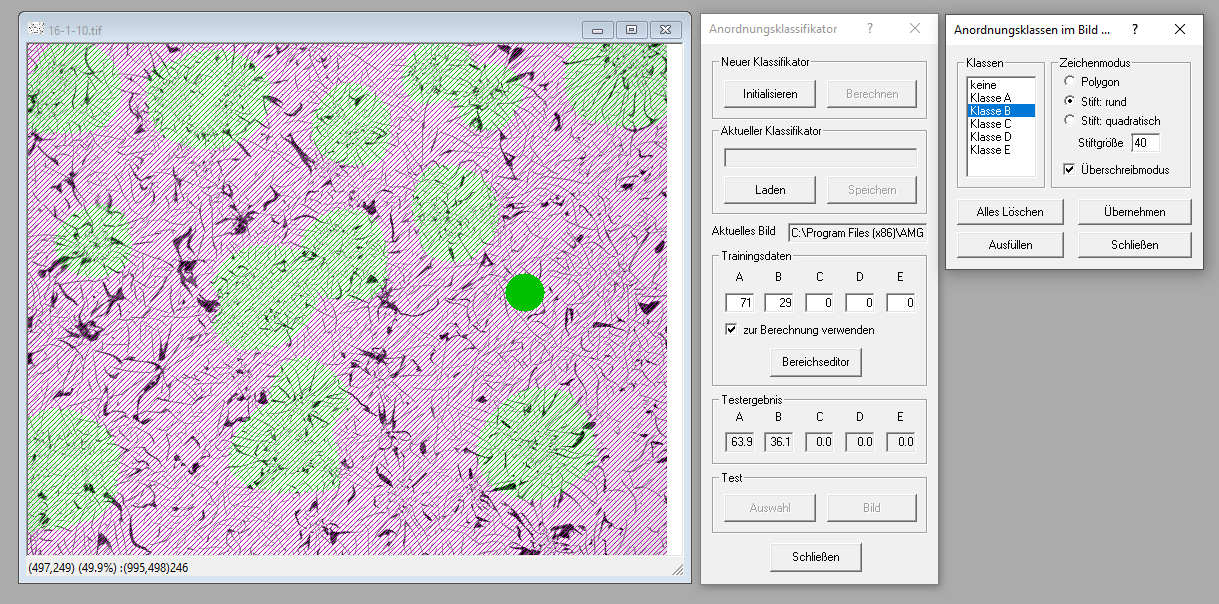
\includegraphics[scale=1.6]{pics/ErstAnordnungsklass}}
	\caption{Erstellung eines Anordnungsklassifikators in AMGuss}
	\label{fig:ErstAnordnungsklass}
\end{figure}

\noindent Grundlage für die Erstellung eines Klassifikators ist eine bereits geladene Bildserie, die zuvor erstellt worden sein muss. Dabei ist anzugeben, mit welcher Kalibrierung  die Bilder der Serie aufgenommen wurden. Diese ist, wie in Kapitel \ref{subsec:Lichtmikroskopie} bereits gezeigt wurde,  abhängig von der Chipgröße der verwendeten Kamera (z.B. $\nicefrac{1}{2}$ Zoll in der Diagonale)  sowie der eingesetzten Optik bestehend aus Lichtweg, Objektiv und Zwischenadapter. Das in Abbildung \ref{fig:ErstAnordnungsklass} (links) dargestellte Bild einer Lamellenguss-Probe hat bspw. eine Kalibrierung von $1~\mu m/\text{Pixel}$. 
\\\\
Im kleinen Fenster (oben rechts) lässt sich dann eine Anordnungsklasse auswählen, der gewünschte Markierungsstil einstellen und die gemäß der gewählten Anordnungsklasse vorkommenden Strukturen im Bild entsprechend markieren. Im Bild links ist dies an den hellgrün markierten Strukturen zu erkennen. Hat der Nutzer dann (ggf. auch in mehreren Bildern) Markierungen für die Anordnungsklassen A bis E hinzugefügt, wird über die Funktion „Initialisieren“ (im mittleren Fenster oben) ein Anordnungsklassifikator erstellt. Dieser kann dann abgespeichert und für Vermessungen von Bildern verwendet werden, deren Kalibrierung dieselbe ($\pm$ eines einstellbaren minimalen Abweichungsfaktors) ist wie die der Bilder, die zur Erstellung des Anordnungsklassifikators verwendet wurden. 
\\\\
\textcolor{red}{$\to$ Vllt. ein Beispiel eines Klassifikators in den Anhang???}

\subsection{Durchführung einer Lamellengraphit-Auswertung mit AMGuss}
\label{subsec:LamelloGraphMesssung}
Zur Erfüllung der Zielsetzung in dieser Arbeit ist eine umfangreiche statistische Analyse durchzuführen, wobei die Daten dafür mit der Software AMGuss generiert werden müssen. Dazu werden sehr viele Messungen notwendig sein, weshalb die Vorgehensweise zur Durchführung einer Messung mit dieser Software hier auch einmal im Detail beschrieben werden soll. Aufbauend darauf wird dann in Kapitel \ref{subsec:Modellierung} ab Seite \pageref{subsec:Modellierung} gezeigt, wie diese Messungen unter Verwendung von AUTOIT (einer Skriptsprache zur automatisierten Steuerung von Windows-Benutzeroberflächen) vollständig automatisiert durchgeführt werden können, was im Rahmen dieser Arbeit dann schließlich auch umgesetzt wird.
\\\\
Um eine Lamellenguss-Auswertung mit der Software AMGuss durchzuführen, müssen folgende Voraussetzungen erfüllt sein:

\begin{enumerate}
	\item Es muss ein oder mehrere Probenbilder mit Lamellengraphit vorliegen und die Kalibrierung in $\nicefrac{\mu m}{\text{Pixel}}$ muss bekannt sein, 
	\item es muss ein Anordnungsklassifikator für eine Bildkalibrierung erstellt worden sein, die der des zu messenden Probebildes entspricht (vgl. dazu auch Kapitel \ref{subsec: ErstellungAnordnungsklassifAMGuss}) und
	\item die zu messenden Bilder sollten in einer AMGuss-Bildserie (.cia-Datei) vorliegen.	
\end{enumerate}

\noindent Abbildung \ref{fig:ImgCalib10} zeigt das Beispiel eines vorliegenden Probenbildes mit Lamellengraphit, welches eine Kalibrierung von $1,0~\nicefrac{\mu m}{\text{Pixel}}$ besitzt.

\begin{figure}[H]
	\centering
	\boxed{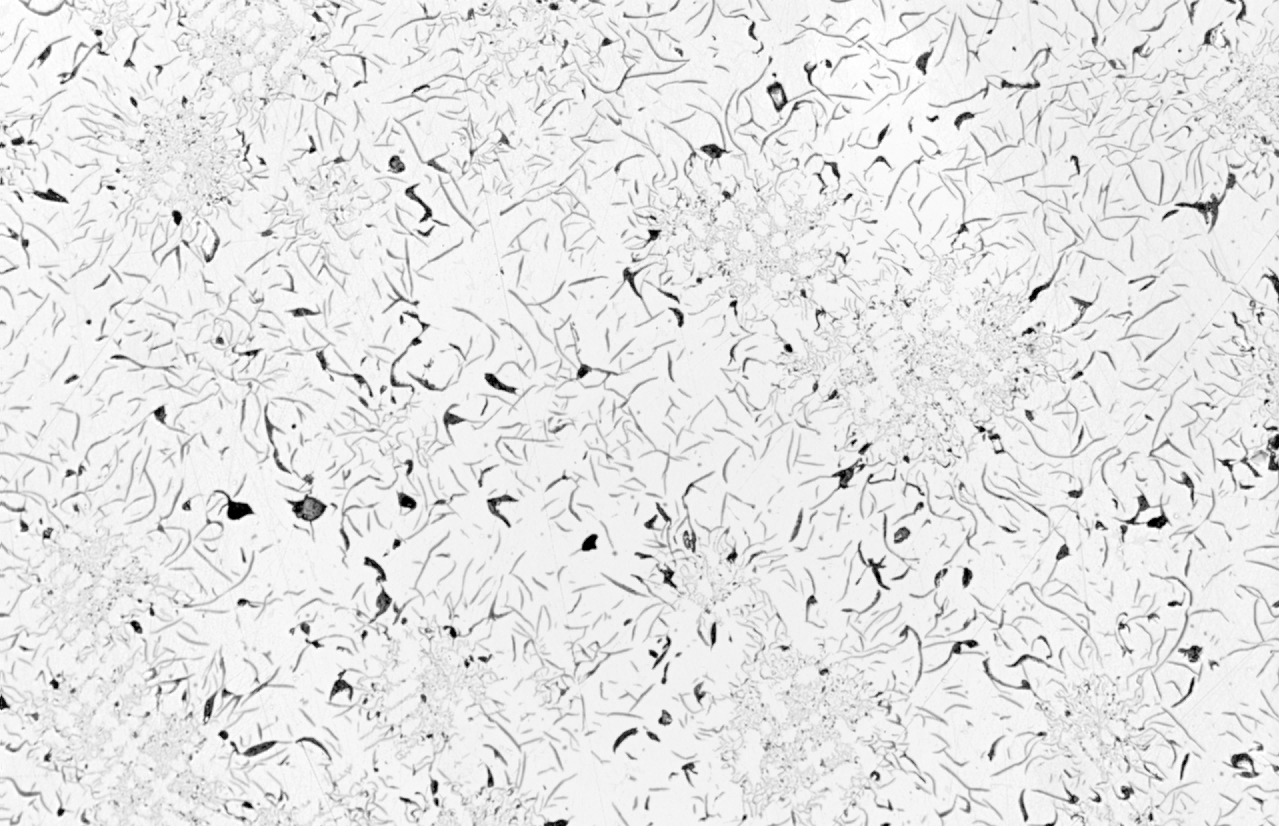
\includegraphics[scale=0.299]{pics/ImgCalib10}}
	\caption{Probenbild mit einer Kalibrierung von $1,0~\nicefrac{\mu m}{\text{Pixel}}$}
	\label{fig:ImgCalib10}
\end{figure}

\noindent Es wird an dieser Stelle vorausgesetzt, das bereits ein Anordnungsklassifikator für diese Kalibrierung erstellt wurde und daher an dieser Stelle nicht mehr weiter darauf eingegangen.
\\\\
\noindent Was nun in Vorbereitung auf die Durchführung der Messung zu tun ist, ist die Erstellung einer Bildserie mit AMGuss. Eine solche kann ein oder mehrere Bilder beinhalten und wird folgendermaßen erstellt:
\\\\
\noindent Zunächst wird das Bild mit AMGuss geöffnet und über den Dialog \textbf{\glqq Neue Bildserie\grqq}~zu einer neuen Bildserie hinzugefügt (Aktives Bild in die Bildserie einfügen), wie in folgender Abbildung \ref{fig:ImgAddToSet} dargestellt.

\begin{figure}[H]
	\centering
	\boxed{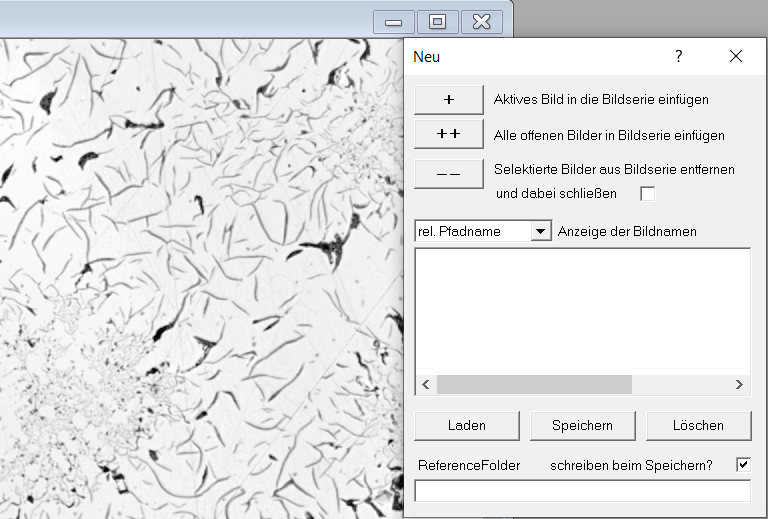
\includegraphics[scale=0.5]{pics/ImgAddToSet}}
	\caption{Probenbild mit einer Kalibrierung von $1,0~\nicefrac{\mu m}{\text{Pixel}}$}
	\label{fig:ImgAddToSet}
\end{figure}

\noindent Das Bild wird daraufhin der Bildserie hinzugefügt wie am linken unteren Rand der Benutzeroberfläche zu erkennen (Abbildung \ref{fig:ImgPicBar}). Die Serie kann nun über den selben Dialog abgespeichert werden (Abbildung \ref{fig:ImgSetSave}).

\begin{minipage}{1.0\linewidth}
	\begin{minipage}[t]{0.3\linewidth}\vspace{0pt}
		\begin{figure}[H]
			\boxed{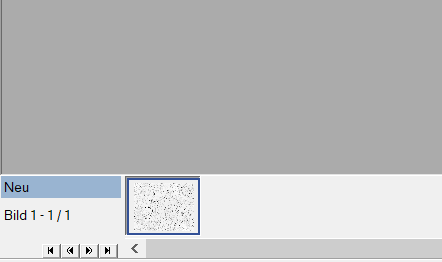
\includegraphics[scale=0.55]{pics/ImgAddedToSet}}
			\caption{Probenbild mit einer Kalibrierung von $1,0~\nicefrac{\mu m}{\text{Pixel}}$}
			\label{fig:ImgPicBar}
		\end{figure}
	\end{minipage}
	\begin{minipage}[t]{0.69\linewidth}\vspace{0pt}
		\begin{figure}[H]
			\centering
			\boxed{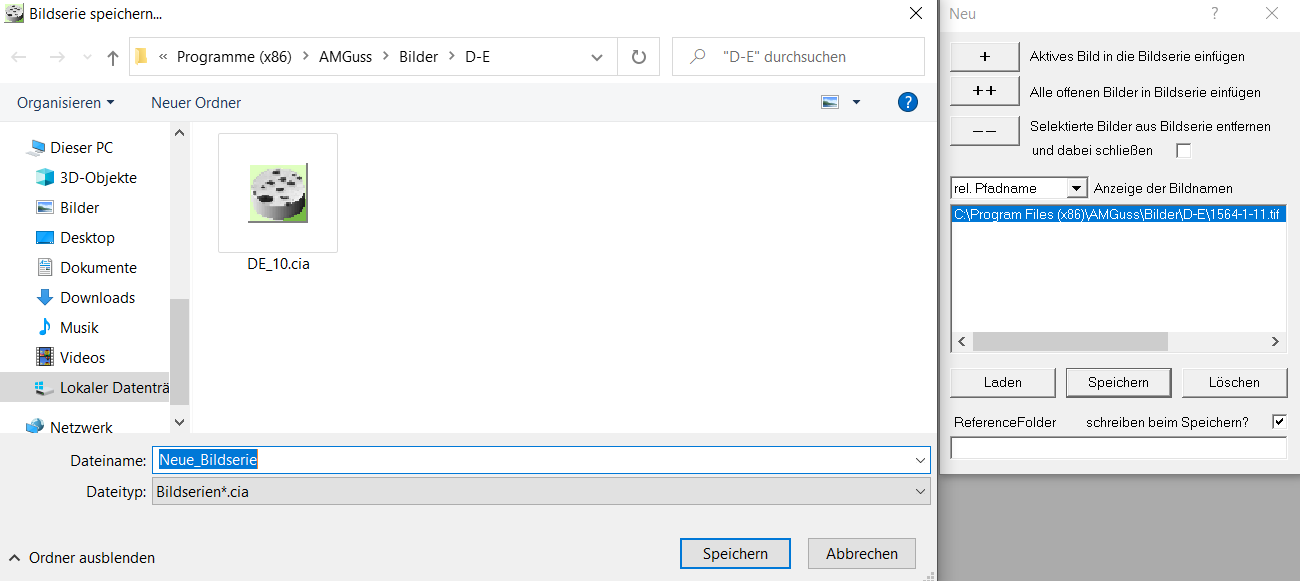
\includegraphics[scale=0.4]{pics/ImgSetSave}}
			\caption{Probenbild mit einer Kalibrierung von $1,0~\nicefrac{\mu m}{\text{Pixel}}$}
			\label{fig:ImgSetSave}
		\end{figure}
	\end{minipage}
\end{minipage}
\\\\\\
\noindent Danach muss die gespeicherte Bildserie über den Dialog \textbf{\glqq Bildserie öffnen\grqq} geöffnet und die Kalibrierung für das Bild in dieser Serie über den Dialog \textbf{\glqq Kalibrierung für Bildserie \grqq} eingegeben werden (Abbildung \ref{fig:ImgSetCalibration}). Der Schritt ist sehr wichtig, da die Software diese Information unbedingt benötigt, um bestimmungsgemäß arbeiten zu können. 

\begin{figure}[H]
	\centering
	\boxed{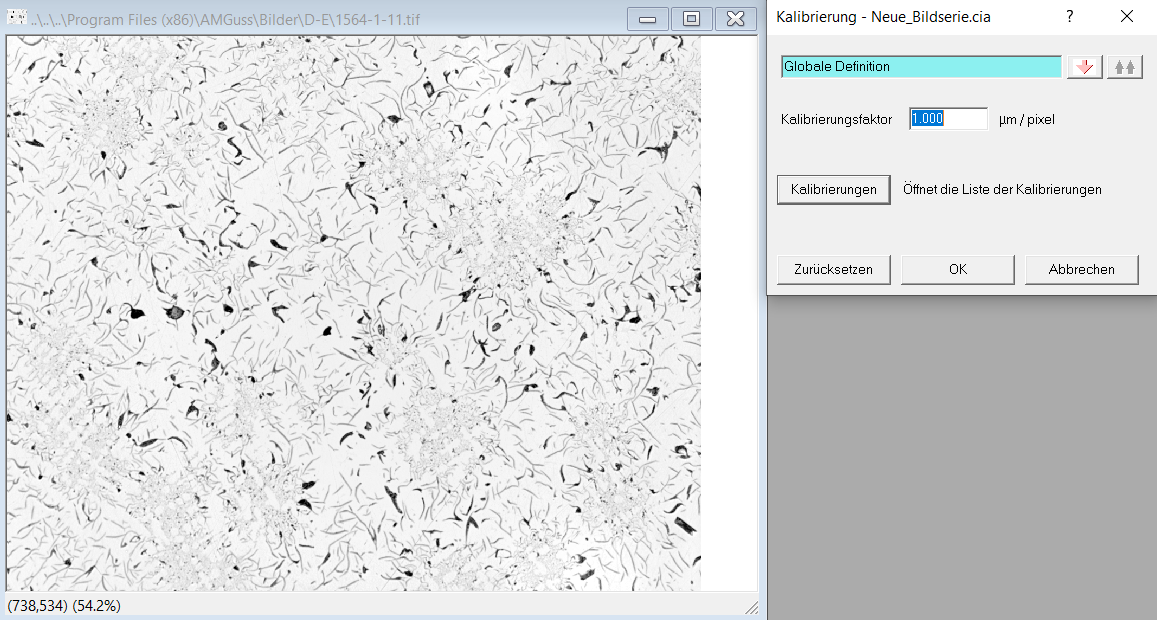
\includegraphics[scale=0.35]{pics/ImgSetCalibration}}
	\caption{Festlegung der Kalibrierung für eine neue Bildserie}
	\label{fig:ImgSetCalibration}
\end{figure}

\noindent Die Bildserie muss danach erneut über den Dialog \textbf{\glqq Bildserien speichern\grqq} abgespeichert werden.
\\\\

\noindent In diesem Fall enthält die Serie nur ein Bild. Bei mehreren Bildern werden auch diese hier entsprechend aufgeführt.
\\\\
Somit sind aller erforderlichen Schritte  erledigt und die Lamellengraphit-Auswertung kann nun durchgeführt werden. Über die Schaltfläche \textbf{\glqq Lamellenguss-Auswertung starten\grqq} muss zunächst bestätigt werden, dass die bereits geöffnete Bildserie Für die Messung verwendet werden soll. Danach erscheint der Dialog zur Auswahl eines Anordnungsklassifikators, der für diese Messung verwendet werden soll.Danach erscheint das in Abbildung \ref{fig:LamelloResultWindowBlank} dargestellte Ergebnisfenster.

\begin{figure}[H]
	\centering
	\boxed{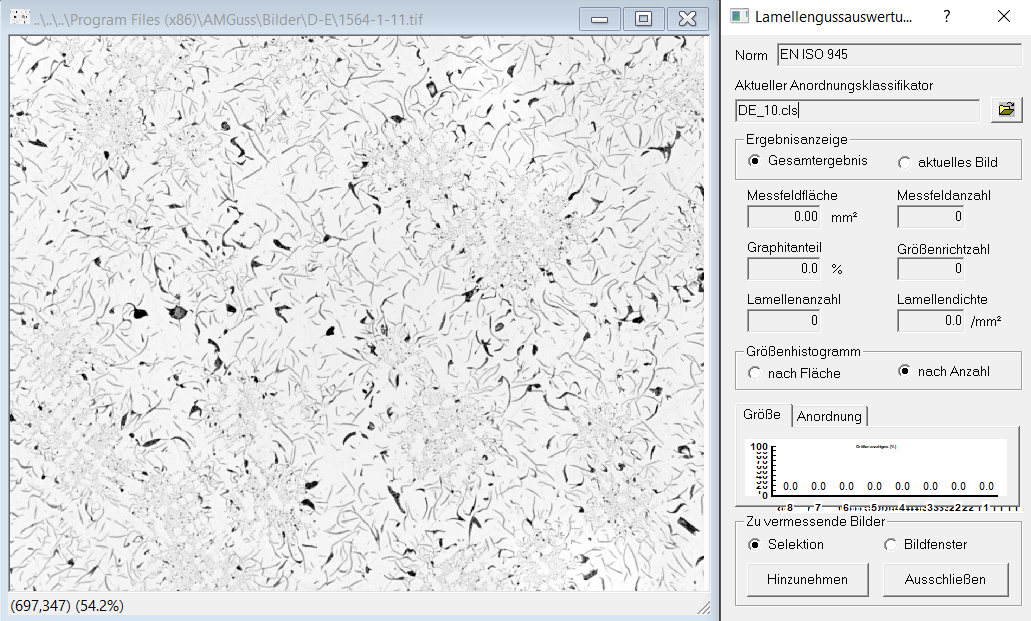
\includegraphics[scale=0.6]{pics/LamelloResultWindowBlank}}
	\caption{Starten einer Lamellenguss-Messung mit AMGuss}
	\label{fig:LamelloResultWindowBlank}
\end{figure}

\noindent Über die Schaltfläche \textbf{\glqq Hinzunehmen\grqq} können die gewünschten Bilder zur Messung hinzugefügt und der Messvorgang gestartet werden. Das Ergebnis zeigt Abbildung \ref{fig:LamelloResult}.

\begin{figure}[H]
	\centering
	\boxed{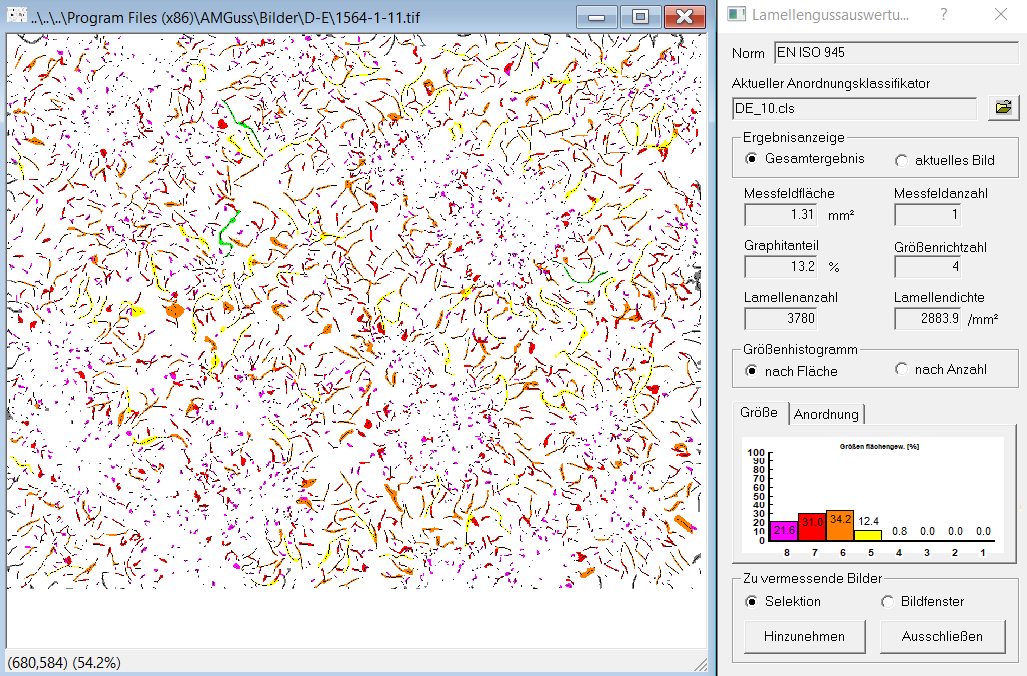
\includegraphics[scale=0.6]{pics/LamelloResultArea}}
	\caption{Ergebnisdarstellung (flächengewichtet) nach Durchführung einer Lamellenguss-Messung}
	\label{fig:LamelloResultArea}
\end{figure}

\noindent Im Histogramm sind die gemessenen Flächenanteile nach Größenklassen dargestellt. Die Ansicht kann mit der Schaltfläche \textbf{\glqq Anordnung\grqq} umgeschaltet und die nach Anordnungsklassen gewichteten Anteile angezeigt werden (Abbildung \ref{fig:LamelloResultArrangementClasses}).

\begin{figure}[H]
	\centering
	\boxed{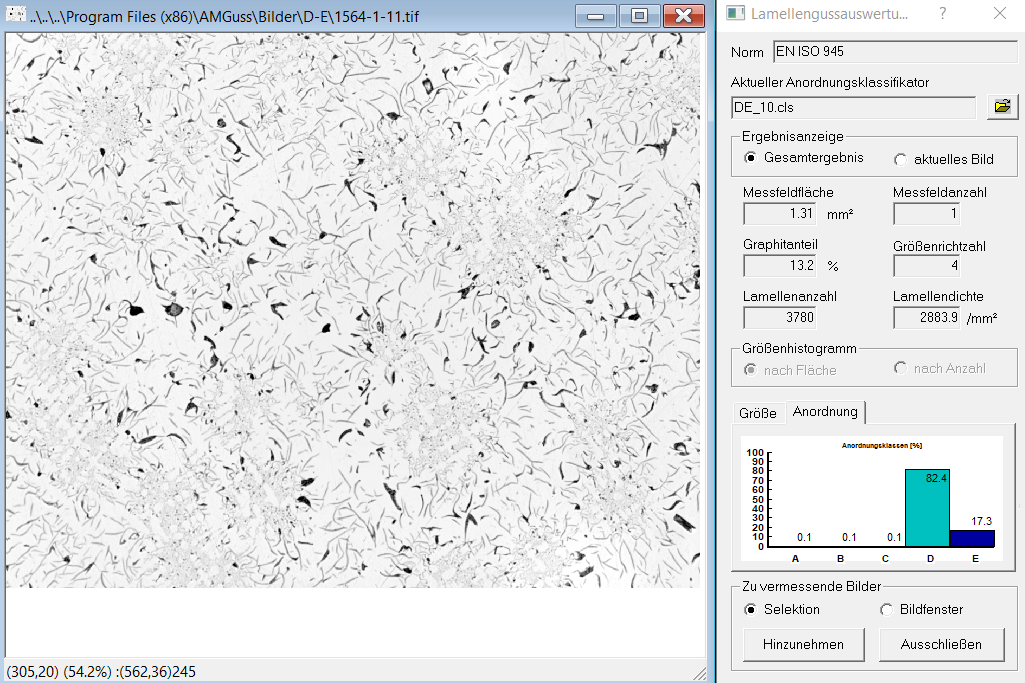
\includegraphics[scale=0.6]{pics/LamelloResultArrangementClasses}}
	\caption{Ergebnisdarstellung (nach Anordnungsklassen) nach Durchführung einer Lamellenguss-Messung}
	\label{fig:LamelloResultArrangementClasses}
\end{figure}

\noindent Aus diesem Messergebnis lässt sich dann schließlich über die Schaltfläche \textbf{\glqq Anzeige und Ausgabe des Messprotokolls\grqq}, nach Auswahl des gewünschten Protokoll-Layouts und Bestätigung der Schaltfläche \textbf{\glqq Protokoll anzeigen\grqq} ein Messprotokoll zur Dokumentation der durchgeführten Messung erzeugen (Abbildung \ref{fig:LamelloReport}).

\begin{figure}[H]
	\centering
	\boxed{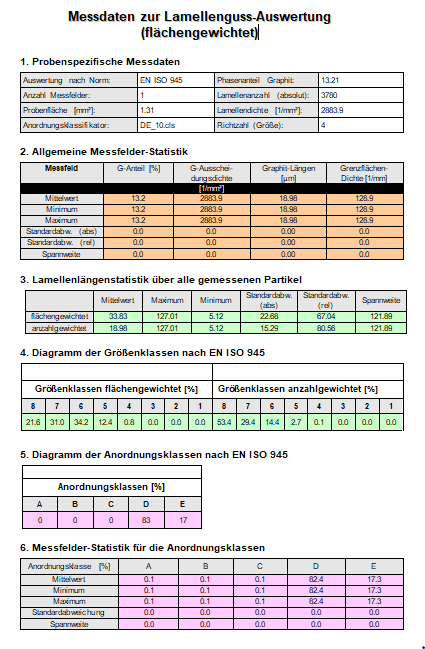
\includegraphics[scale=0.8]{pics/LamelloReport}}
	\caption{Darstellung eines AMGuss-Messprotokolls}
	\label{fig:LamelloReport}
\end{figure}

\noindent Im nächsten Abschnitt dieses Kapitels werden nun die hier dargestellten Messergebnisse einer genaueren Betrachtung unterzogen.

\subsection{Erläuterungen zum Verständnis der Messergebnisse einer Lamellengraphit-Auswertung}
\label{subsec:ErgebnisseAMGuss}
Im folgenden werden die Messergebnisse aus den in Abbildung \ref{fig:LamelloReport} dargestellten Messprotokolle entschlüsselt und die Bedeutung einzelner Werte genauer beschrieben. Dabei wird nicht zwischen a) und b) unterschiedenen, da die Werte in beiden Protokollen



\section{Zur Verfügung stehendes Bildmaterial}
\label{subsec:Bildmaterial}

\section{Problemstellung}
\label{sec:Problemstellung}

Die Forderung nach Allgemeingültigkeit bei einem Anordnungsklassifikator in diesem Kontext zu erfüllen bedeutet, einen Algorithmus zu implementieren, mit dem die Kalibrierung der für eine Messung vorliegenden Bilder an die mit dem ein im System hinterlegter Anordnungsklassifikator erstellt wurde, anzupassen. Das kann grundsätzlich durch Skalierung erreicht werden. Da sich die Kalibrierung umgekehrt Proportional zur Bildgröße verhält müsste zum Beispiel ein mit einer Ausgangskalibrierung von $1,0~\nicefrac{\mu m}{\text{Pixel}}$ vorliegendes Bild also um den Faktor 2 hoch-skaliert (vergrößert) werden, um die Kalibrierung auf $0,5~\nicefrac{\mu m}{\text{Pixel}}$ zu verändern. Analog dazu wäre es dann natürlich auch möglich, eine zu große Ausgangskalibrierung durch Verkleinerung des Bildes entsprechend anzupassen. Geht man weiter davon aus, das der im System hinterlegte Anordnungsklassifikator mit Bildern derselben Kalibrierung erstellt wurde, wäre nun eine korrekte Messung mit diesem Klassifikator möglich. Somit würde der Arbeitsschritt zur manuellen Erstellung und Verwaltung von Klassifikatoren für unterschiedliche Ausgangskalibrierungen wegfallen und die Forderung nach Allgemeingültigkeit wäre damit erfüllt und man würde mit nur einem einzigen Anordnungsklassifikator auskommen.
\\\\
Bei der Skalierung von Bildern ist jedoch zu beachten, das zur Erhaltung der Bildqualität verschiedene Interpolationsalgorithmen zum Einsatz kommen um die sich durch Vergrößerung/Verkleinerung ergebende Differenz der Pixelanzahl zwischen Eingangs- und Ausgangsbild auszugleichen. Im Falle der Vergrößerung ergibt sich, dass das Ausgangsbild entsprechend dem Vergrößerungsfaktor mehr Pixel besitzt als das Eingangsbild und die sich dadurch ergebenden Pixellücken durch Interpolation gefüllt werden müssen. Bei Verkleinerung verhält es sich genau umgekehrt, nur das in diesem Fall die Pixelmenge verkleinert wird. Es liegt auf der Hand, das eine solche Interpolation die Details des Originalbildes nie 100\%-ig erhalten kann. So können zwar für viele praktischen Anwendungsfälle im Grafik- oder Fotobereich sehr gute Ergebnisse erzielt werden, weil das menschliche Auge diese Abweichungen nicht erkennen kann. Allerdings erweist sich die Interpolation im Bereich der bildbasierten Materialstrukturanalyse als problematisch, da sich  die zu analysierenden Strukturen durch die Interpolation verändern und somit die Messergebnisse verfälscht werden. Welche unerwünschten Auswirkungen das im vorliegenden Fall hat, zeigen die folgenden Abbildungen \ref{fig:KlassErrorVisuell} und \ref{fig:KlassErrorHisto}.

\begin{figure}[h]
	\label{fig:KlassErrorVisuell}
	\begin{subfigure}{0.33\textwidth}
		\centering
		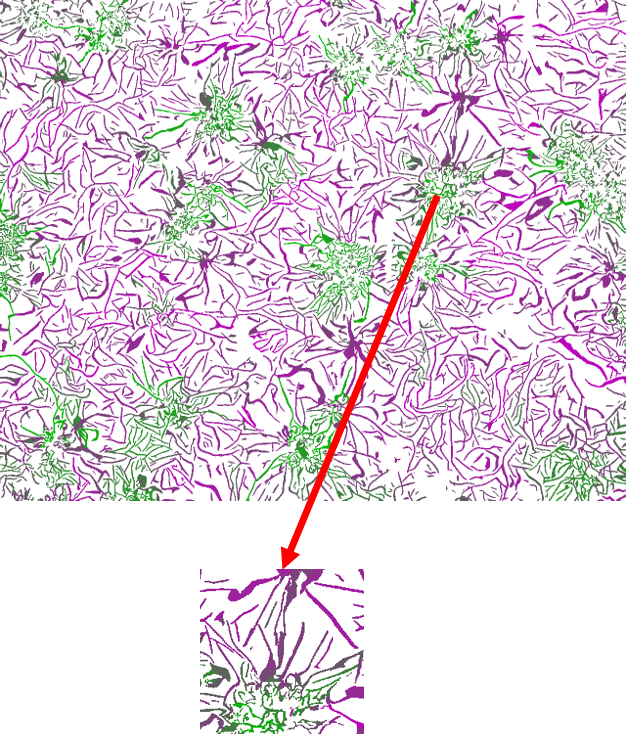
\includegraphics[scale=0.5]{pics/ClassificationCalib10.png}
		\caption{Ausgangsbild mit Kalibrierung 1,0}
	\end{subfigure}\hfill
	\begin{subfigure}{0.33\textwidth}
		\centering
		\begin{tikzpicture}[x=0.75pt,y=0.75pt,yscale=-1,xscale=1]
			%uncomment if require: \path (0,300); %set diagram left start at 0, and has height of 300
			
			%Right Arrow [id:dp9517904043992672] 
			\draw  [color={rgb, 255:red, 208; green, 2; blue, 27 }  ,draw opacity=1 ][fill={rgb, 255:red, 255; green, 255; blue, 255 }  ,fill opacity=1 ][line width=1.5]  (192,87.35) -- (273.83,87.35) -- (273.83,65.85) -- (328.38,108.85) -- (273.83,151.85) -- (273.83,130.35) -- (192,130.35) -- cycle ;
			
			% Text Node
			\draw (198,97) node [anchor=north west][inner sep=0.75pt]  [font=\tiny] [align=left] {Änderung der Kalibrierung\\von 1,0 auf 0,5 = Skalierung\\um den Faktor 2};
		\end{tikzpicture}
	\end{subfigure}\hfill
	\begin{subfigure}{0.33\textwidth}
		\centering
		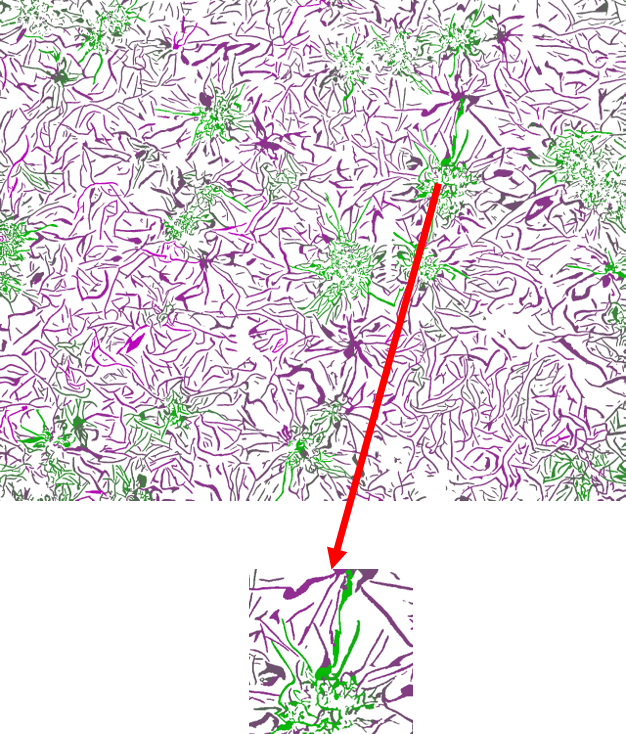
\includegraphics[scale=0.5]{pics/ClassificationCalib05.png}
		\caption{Transform. Bild mit Kalibrierung 0,5}
	\end{subfigure}
	\caption{Messfehler-Darstellung (visuell) nach Bildtransformation mit bikubischer Interpolation}
	\label{fig:KlassErrorVisuell}
\end{figure}

\begin{figure}[h]
	\begin{subfigure}{0.33\textwidth}
		\centering
		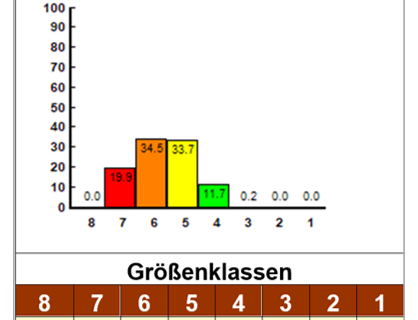
\includegraphics[scale=0.5]{pics/HistoCalib10}
		\caption{Ausgangsbild mit Kalibrierung 1,0}
	\end{subfigure}\hfill
	\begin{subfigure}{0.33\textwidth}
		\centering
		\begin{tikzpicture}[x=0.75pt,y=0.75pt,yscale=-1,xscale=1]
			%uncomment if require: \path (0,300); %set diagram left start at 0, and has height of 300
			
			%Right Arrow [id:dp9517904043992672] 
			\draw  [color={rgb, 255:red, 208; green, 2; blue, 27 }  ,draw opacity=1 ][fill={rgb, 255:red, 255; green, 255; blue, 255 }  ,fill opacity=1 ][line width=1.5]  (192,87.35) -- (273.83,87.35) -- (273.83,65.85) -- (328.38,108.85) -- (273.83,151.85) -- (273.83,130.35) -- (192,130.35) -- cycle ;
			
			% Text Node
			\draw (198,97) node [anchor=north west][inner sep=0.75pt]  [font=\tiny] [align=left] {Änderung der Kalibrierung\\von 1,0 auf 0,5 = Skalierung\\um den Faktor 2};
		\end{tikzpicture}
	\end{subfigure}\hfill
	\begin{subfigure}{0.33\textwidth}
		\centering
		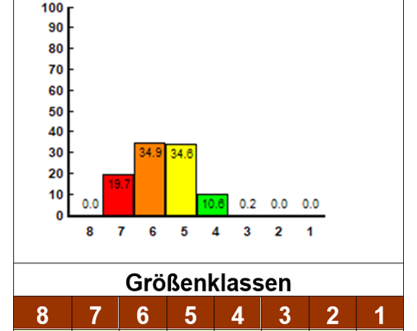
\includegraphics[scale=0.5]{pics/HistoCalib05.png}
		\caption{Transform. Bild mit Kalibrierung 0,5}
	\end{subfigure}
	\caption{Messfehler-Darstellung (Histogramm) nach Bildtransformation mit bikubischer Interpolation}
	\label{fig:KlassErrorHisto}
\end{figure}

\newpage

\noindent Es wurde also ein Bild mit einer Ausgangskalibrierung von $1,0~\nicefrac{\mu m}{\text{Pixel}}$ um den Faktor 2 mit dem Ziel skaliert, die Kalibrierung auf $0,5~\nicefrac{\mu m}{\text{Pixel}}$ zu verändern. Die beiden Abbildungen zeigen nun unterschiedliche Sichtweisen auf ein und dasselbe Problem. Bereits in Bild 3.5 visuell erkennbare Klassifikationsfehler, tauchen auch in dem von AMGuss errechneten Analyseergebnis auf und sind an einer leichten Linksverschiebung der Histogrammdaten zu erkennen. Die Fehler sind zwar im hier betrachteten Fall sehr gering, im Bereich der Materialstrukturanalyse sehr unerwünscht, da sich aus der Lage, Größe und Verteilung (also der Gesamtstruktur) mechanische Materialeigenschaften(bspw. Druck und Zugfestigkeit, Bruchsicherheit, etc.) ableiten lassen und somit diese Abweichungen zu Fehleinschätzungen bei der qualitativen Bewertung des Materials führen können.

\chapter{Konzept}
\label{ch:Konzept}

\section{Sollzustand/Anforderungen}
\label{sec:DefAnforderungenAnordnKlas}
Die Vorgehensweise zur Erstellung eines Anordnungsklassifikators wurde in Kapitel \ref{subsec: ErstellungAnordnungsklassifAMGuss} bereits beschrieben. Dies ist für den Nutzer mit einem nicht unerheblichen Aufwand verbunden. Hinzu kommt eine gewisse Fehleranfälligkeit, da für jede Messung der in Bezug auf die Bildkalibrierung richtige Klassifikator für die Messung ausgewählt werden muss.
\\\\
\noindent Das Gütekriterium an einen allgemeingültigen Klassifikator ist, die durch Skalierung (bzw. Interpolation) hervorgerufenen und in Kapitel \ref{sec:Problemstellung} bereits näher beschriebenen Messfehler auf ein \textbf{tolerierbares} Maß hin zu minimieren. Allerdings gibt es jedoch, nach den aktuellen allgemein anerkannten Regeln der Technik, keinen eindeutigen objektiven Maßstab, der zur Beurteilung angelegt werden könnte. Stattdessen beruht die Graphitklassifizierung auf einer visuellen Einschätzung der Spezialisten, welche die Beurteilung der Proben vornehmen. Die Norm DIN ISO 945-1 definiert dabei die Grundlagen, auf denen eine solche Beurteilung zu erfolgen hat. Was also als noch tolerierbar gilt, entscheidet der versierte Nutzer in gewissen Grenzen selbst und wie die Erfahrungen zeigen, existieren teils nicht unerhebliche Abweichungen bei der Einschätzung. Die im Rahmen dieser Arbeit zu erfüllenden Anforderungen lassen sich daher wie folgt beschreiben:
\\\\
\noindent Die Aufgabe besteht darin zu untersuchen und nachzuweisen, wie sich die Anwendung verschiedener Interpolationsalgorithmen bei der Bildtransformation bzw. Veränderung der Bildskalierungen auf die Messgenauigkeit bei der Durchführung von Lamellengraphitauswertungen mit der Software AMGuss auswirken. 

\section{Erzeugung von Bildern mit unterschiedlichen Ausgangskalibrierungen}
\label{sec:ErzeugungVonBildern}
\begin{figure}[H]
	\centering
	\begin{tikzpicture}[x=0.75pt,y=0.75pt,yscale=-1,xscale=1, scale=0.7, every node/.style={scale=0.7}]
		%uncomment if require: \path (0,222); %set diagram left start at 0, and has height of 222
		
		%Straight Lines [id:da8513951726256912] 
		\draw [line width=0.75]  [dash pattern={on 0.84pt off 2.51pt}]  (252,80) -- (252,320) ;
		%Straight Lines [id:da5456588557389066] 
		\draw [line width=1.5]    (172,420) -- (412,420) ;
		%Straight Lines [id:da6601013014749395] 
		\draw [line width=1.5]    (172,180) -- (172,420) ;
		%Straight Lines [id:da3287587582519509] 
		\draw [line width=1.5]    (172,180) -- (412,180) ;
		%Straight Lines [id:da8891201835694393] 
		\draw [line width=1.5]    (252,80) -- (172,180) ;
		%Straight Lines [id:da8301479230800961] 
		\draw [line width=1.5]    (492,80) -- (412,180) ;
		%Straight Lines [id:da897285446062482] 
		\draw [line width=1.5]    (492,320) -- (412,420) ;
		%Straight Lines [id:da291618853913844] 
		\draw [line width=1.5]    (492,80) -- (492,320) ;
		%Straight Lines [id:da27301051400697607] 
		\draw [line width=1.5]    (252,80) -- (492,80) ;
		%Straight Lines [id:da03595133060933242] 
		\draw [line width=0.75]  [dash pattern={on 0.84pt off 2.51pt}]  (252,320) -- (492,320) ;
		%Straight Lines [id:da5805598360719648] 
		\draw [line width=0.75]  [dash pattern={on 0.84pt off 2.51pt}]  (252,320) -- (172,420) ;
		%Straight Lines [id:da6408604526403883] 
		\draw    (291,414) -- (291,427) ; 				% 1.10
		%Straight Lines [id:da5720641419192563] 
		\draw [color={rgb, 255:red, 208; green, 2; blue, 27 }  ,draw opacity=1 ]   (201,414) -- (201,427) ;			% 0.50
		%Straight Lines [id:da7586148570180449] 
		\draw    (231,414) -- (231,427) ; 				% 0.70
		%Straight Lines [id:da6213998766294877] 
		\draw    (412,414) -- (412,427) ; 				% 1.90
		%Straight Lines [id:da21868777946411622] 
		\draw    (172,414) -- (172,427) ;				% 0.30
		%Shape: Parallelogram [id:dp6855290487769707] 
		\draw  [fill={rgb, 255:red, 126; green, 211; blue, 33 }  ,fill opacity=0.83 ] (252,200) -- (492,200) -- (412,300) -- (172,300) -- cycle ;
		%Shape: Square [id:dp5568502450606261] 
		\draw  [fill={rgb, 255:red, 74; green, 74; blue, 74 }  ,fill opacity=1 ] (304,224) -- (374,224) -- (374,294) -- (304,294) -- cycle ;
		%Shape: Square [id:dp11497079395910248] 
		\draw  [fill={rgb, 255:red, 74; green, 74; blue, 74 }  ,fill opacity=1 ] (294,234) -- (364,234) -- (364,304) -- (294,304) -- cycle ;
		%Shape: Square [id:dp9507633897127776] 
		\draw  [fill={rgb, 255:red, 74; green, 74; blue, 74 }  ,fill opacity=1 ] (285,244) -- (355,244) -- (355,314) -- (285,314) -- cycle ;
		%Shape: Square [id:dp2885472363956254] 
		\draw  [fill={rgb, 255:red, 74; green, 74; blue, 74 }  ,fill opacity=1 ] (273,256) -- (343,256) -- (343,326) -- (273,326) -- cycle ;
		%Shape: Square [id:dp9167567864275155] 
		\draw  [fill={rgb, 255:red, 74; green, 74; blue, 74 }  ,fill opacity=1 ] (262,268) -- (332,268) -- (332,338) -- (262,338) -- cycle ;
		
		%Straight Lines [id:da21914875225668995] 
		\draw [line width=1.5]    (412,180) -- (412,420) ;
		
		% Text Node
		\draw (276,284) node [anchor=north west][inner sep=0.75pt]  [color={rgb, 255:red, 255; green, 255; blue, 255 }  ,opacity=1 ] [align=left] {\begin{minipage}[lt]{28.8pt}\setlength\topsep{0pt}
				\begin{center}
					232\\Bilder
				\end{center}
				
		\end{minipage}};
		% Text Node
		\draw (506,199.71) node [anchor=north] [inner sep=0.75pt]  [font=\normalsize,rotate=-270] [align=left] {\textbf{Interpolationsmodi}};
		% Text Node
		\draw (159,430) node [anchor=north west][inner sep=0.75pt]  [font=\scriptsize] [align=left] {0,30};
		% Text Node
		\draw (190,430) node [anchor=north west][inner sep=0.75pt]  [font=\scriptsize,color={rgb, 255:red, 208; green, 2; blue, 27 }  ,opacity=1 ] [align=left] {0,50};
		% Text Node
		\draw (220,430) node [anchor=north west][inner sep=0.75pt]  [font=\scriptsize] [align=left] {0,70};
		% Text Node
		\draw (280,430) node [anchor=north west][inner sep=0.75pt]  [font=\scriptsize] [align=left] {1,10};
		% Text Node
		\draw (400,430) node [anchor=north west][inner sep=0.75pt]  [font=\scriptsize] [align=left] {1,90};
		% Text Node
		\draw (197,408) node [anchor=north west][inner sep=0.75pt]  [font=\scriptsize, rotate=52.5,color={rgb, 255:red, 208; green, 2; blue, 27 }  ,opacity=1 ] [align=left] {Zielkalibrierung};
		% Text Node
		\draw (438,410) node [anchor=north west][inner sep=0.75pt]   [align=left] {{\scriptsize - Nearest Neighbor}};
		% Text Node
		\draw (461,380) node [anchor=north west][inner sep=0.75pt]  [font=\scriptsize] [align=left] {\mbox{-} Linear};
		% Text Node
		\draw (483,349) node [anchor=north west][inner sep=0.75pt]  [font=\scriptsize] [align=left] {\mbox{-} Cubic};
		% Text Node
		\draw (492,334) node [anchor=north west][inner sep=0.75pt]  [font=\scriptsize] [align=left] {\mbox{-} Area};
		% Text Node
		\draw (501,322) node [anchor=north west][inner sep=0.75pt]  [font=\scriptsize] [align=left] {\mbox{-} Lanczos};
		% Text Node
		\draw (450,394) node [anchor=north west][inner sep=0.75pt]   [align=left] {{\scriptsize - Nearest Neighbor} {\scriptsize / Exact}};
		% Text Node
		\draw (472,364) node [anchor=north west][inner sep=0.75pt]  [font=\scriptsize] [align=left] {\mbox{-} Linear / Exact};
		% Text Node
		\draw (203,450) node [anchor=north west][inner sep=0.75pt]  [font=\normalsize] [align=left] {\textbf{Ausgangskalibrierungen}};
		% Text Node
		\draw (138.21,183.34) node [anchor=north west][inner sep=0.75pt]  [font=\normalsize,rotate=-308.72] [align=left] {\textbf{Interpolationsverfahren}};
		% Text Node
		\draw (422.19,183.01) node [anchor=north west][inner sep=0.75pt]  [font=\scriptsize,color={rgb, 255:red, 65; green, 117; blue, 5 }  ,opacity=1 ,rotate=-308.57] [align=left] {\begin{minipage}[lt]{45.99pt}\setlength\topsep{0pt}
				\begin{center}
					\textbf{schrittweise }\\\textbf{Skalierung}
				\end{center}
				
		\end{minipage}};
		% Text Node
		\draw (431.9,300.81) node [anchor=north west][inner sep=0.75pt]  [font=\scriptsize,color={rgb, 255:red, 65; green, 117; blue, 5 }  ,opacity=1 ,rotate=-308.09] [align=left] {\textbf{Vollskalierung}};
	\end{tikzpicture}
	\caption{Planungsmodell (1) zur Erzeugung von Versuchsbildern}
	\label{fig:Planungsmodell(1)}
\end{figure}

\begin{figure}[H]
	\centering
	\begin{tikzpicture}[x=0.75pt,y=0.75pt,yscale=-1,xscale=1, scale=1.0, every node/.style={scale=1.0}]
		%uncomment if require: \path (0,222); %set diagram left start at 0, and has height of 222
		
		%Shape: Rectangle [id:dp6366412495734111] 
		\draw  [fill={rgb, 255:red, 74; green, 74; blue, 74 }  ,fill opacity=1 ] (53.75,200) -- (110,200) -- (110,255.26) -- (53.75,255.26) -- cycle ;
		%Shape: Rectangle [id:dp751718043193554] 
		\draw  [fill={rgb, 255:red, 74; green, 74; blue, 74 }  ,fill opacity=1 ] (45.71,207.89) -- (101.96,207.89) -- (101.96,263.16) -- (45.71,263.16) -- cycle ;
		%Shape: Rectangle [id:dp8955994284702644] 
		\draw  [fill={rgb, 255:red, 74; green, 74; blue, 74 }  ,fill opacity=1 ] (38.48,215.79) -- (94.73,215.79) -- (94.73,271.05) -- (38.48,271.05) -- cycle ;
		%Shape: Rectangle [id:dp5207514318052735] 
		\draw  [fill={rgb, 255:red, 74; green, 74; blue, 74 }  ,fill opacity=1 ] (28.84,225.26) -- (85.09,225.26) -- (85.09,280.53) -- (28.84,280.53) -- cycle ;
		%Shape: Rectangle [id:dp8155725825356159] 
		\draw  [fill={rgb, 255:red, 74; green, 74; blue, 74 }  ,fill opacity=1 ] (20,234.74) -- (76.25,234.74) -- (76.25,290) -- (20,290) -- cycle ;
		%Rounded Rect [id:dp8565749595273766] 
		\draw  [color={rgb, 255:red, 155; green, 155; blue, 155 }  ,draw opacity=1 ][fill={rgb, 255:red, 155; green, 155; blue, 155 }  ,fill opacity=0.12 ] (165,48) .. controls (165,43.58) and (168.58,40) .. (173,40) -- (252,40) .. controls (256.42,40) and (260,43.58) .. (260,48) -- (260,72) .. controls (260,76.42) and (256.42,80) .. (252,80) -- (173,80) .. controls (168.58,80) and (165,76.42) .. (165,72) -- cycle ;
		%Rounded Rect [id:dp6075836530317975] 
		\draw  [color={rgb, 255:red, 155; green, 155; blue, 155 }  ,draw opacity=1 ][fill={rgb, 255:red, 155; green, 155; blue, 155 }  ,fill opacity=0.12 ] (163,109) .. controls (163,104.58) and (166.58,101) .. (171,101) -- (252,101) .. controls (256.42,101) and (260,104.58) .. (260,109) -- (260,133) .. controls (260,137.42) and (256.42,141) .. (252,141) -- (171,141) .. controls (166.58,141) and (163,137.42) .. (163,133) -- cycle ;
		%Rounded Rect [id:dp0325477461297643] 
		\draw  [color={rgb, 255:red, 155; green, 155; blue, 155 }  ,draw opacity=1 ][fill={rgb, 255:red, 155; green, 155; blue, 155 }  ,fill opacity=0.12 ] (163,169) .. controls (163,164.58) and (166.58,161) .. (171,161) -- (252,161) .. controls (256.42,161) and (260,164.58) .. (260,169) -- (260,193) .. controls (260,197.42) and (256.42,201) .. (252,201) -- (171,201) .. controls (166.58,201) and (163,197.42) .. (163,193) -- cycle ;
		%Rounded Rect [id:dp3162904694467472] 
		\draw  [color={rgb, 255:red, 155; green, 155; blue, 155 }  ,draw opacity=1 ][fill={rgb, 255:red, 155; green, 155; blue, 155 }  ,fill opacity=0.12 ] (163,228) .. controls (163,223.58) and (166.58,220) .. (171,220) -- (252,220) .. controls (256.42,220) and (260,223.58) .. (260,228) -- (260,252) .. controls (260,256.42) and (256.42,260) .. (252,260) -- (171,260) .. controls (166.58,260) and (163,256.42) .. (163,252) -- cycle ;
		%Rounded Rect [id:dp3035992482144214] 
		\draw  [color={rgb, 255:red, 155; green, 155; blue, 155 }  ,draw opacity=1 ][fill={rgb, 255:red, 155; green, 155; blue, 155 }  ,fill opacity=0.12 ] (163,289) .. controls (163,284.58) and (166.58,281) .. (171,281) -- (252,281) .. controls (256.42,281) and (260,284.58) .. (260,289) -- (260,313) .. controls (260,317.42) and (256.42,321) .. (252,321) -- (171,321) .. controls (166.58,321) and (163,317.42) .. (163,313) -- cycle ;
		%Rounded Rect [id:dp2836577100042894] 
		\draw  [color={rgb, 255:red, 155; green, 155; blue, 155 }  ,draw opacity=1 ][fill={rgb, 255:red, 155; green, 155; blue, 155 }  ,fill opacity=0.12 ] (163,349) .. controls (163,344.58) and (166.58,341) .. (171,341) -- (252,341) .. controls (256.42,341) and (260,344.58) .. (260,349) -- (260,373) .. controls (260,377.42) and (256.42,381) .. (252,381) -- (171,381) .. controls (166.58,381) and (163,377.42) .. (163,373) -- cycle ;
		%Rounded Rect [id:dp9146993081319426] 
		\draw  [color={rgb, 255:red, 155; green, 155; blue, 155 }  ,draw opacity=1 ][fill={rgb, 255:red, 155; green, 155; blue, 155 }  ,fill opacity=0.12 ] (163,408) .. controls (163,403.58) and (166.58,400) .. (171,400) -- (252,400) .. controls (256.42,400) and (260,403.58) .. (260,408) -- (260,432) .. controls (260,436.42) and (256.42,440) .. (252,440) -- (171,440) .. controls (166.58,440) and (163,436.42) .. (163,432) -- cycle ;
		%Rounded Rect [id:dp5049349195701525] 
		\draw  [color={rgb, 255:red, 155; green, 155; blue, 155 }  ,draw opacity=1 ][fill={rgb, 255:red, 155; green, 155; blue, 155 }  ,fill opacity=0.12 ] (417,322) .. controls (417,317.58) and (420.58,314) .. (425,314) -- (501,314) .. controls (505.42,314) and (509,317.58) .. (509,322) -- (509,346) .. controls (509,350.42) and (505.42,354) .. (501,354) -- (425,354) .. controls (420.58,354) and (417,350.42) .. (417,346) -- cycle ;
		%Rounded Rect [id:dp7024977089857076] 
		\draw  [color={rgb, 255:red, 155; green, 155; blue, 155 }  ,draw opacity=1 ][fill={rgb, 255:red, 155; green, 155; blue, 155 }  ,fill opacity=0.12 ] (417,141) .. controls (417,136.58) and (420.58,133) .. (425,133) -- (501,133) .. controls (505.42,133) and (509,136.58) .. (509,141) -- (509,165) .. controls (509,169.42) and (505.42,173) .. (501,173) -- (425,173) .. controls (420.58,173) and (417,169.42) .. (417,165) -- cycle ;
		%Rounded Rect [id:dp7889794089989934] 
		\draw  [color={rgb, 255:red, 155; green, 155; blue, 155 }  ,draw opacity=1 ][fill={rgb, 255:red, 155; green, 155; blue, 155 }  ,fill opacity=0.12 ] (417,200) .. controls (417,195.58) and (420.58,192) .. (425,192) -- (501,192) .. controls (505.42,192) and (509,195.58) .. (509,200) -- (509,224) .. controls (509,228.42) and (505.42,232) .. (501,232) -- (425,232) .. controls (420.58,232) and (417,228.42) .. (417,224) -- cycle ;
		%Rounded Rect [id:dp17780665664929307] 
		\draw  [color={rgb, 255:red, 155; green, 155; blue, 155 }  ,draw opacity=1 ][fill={rgb, 255:red, 155; green, 155; blue, 155 }  ,fill opacity=0.12 ] (417,262) .. controls (417,257.58) and (420.58,254) .. (425,254) -- (501,254) .. controls (505.42,254) and (509,257.58) .. (509,262) -- (509,286) .. controls (509,290.42) and (505.42,294) .. (501,294) -- (425,294) .. controls (420.58,294) and (417,290.42) .. (417,286) -- cycle ;
		%Rounded Rect [id:dp08184078829998631] 
		\draw  [color={rgb, 255:red, 155; green, 155; blue, 155 }  ,draw opacity=1 ][fill={rgb, 255:red, 126; green, 211; blue, 33 }  ,fill opacity=1 ] (300,188) .. controls (300,183.58) and (303.58,180) .. (308,180) -- (372,180) .. controls (376.42,180) and (380,183.58) .. (380,188) -- (380,212) .. controls (380,216.42) and (376.42,220) .. (372,220) -- (308,220) .. controls (303.58,220) and (300,216.42) .. (300,212) -- cycle ;
		%Rounded Rect [id:dp9437055363891322] 
		\draw  [color={rgb, 255:red, 155; green, 155; blue, 155 }  ,draw opacity=1 ][fill={rgb, 255:red, 126; green, 211; blue, 33 }  ,fill opacity=1 ] (301,269) .. controls (301,264.58) and (304.58,261) .. (309,261) -- (374,261) .. controls (378.42,261) and (382,264.58) .. (382,269) -- (382,293) .. controls (382,297.42) and (378.42,301) .. (374,301) -- (309,301) .. controls (304.58,301) and (301,297.42) .. (301,293) -- cycle ;
		%Straight Lines [id:da4572029334299341] 
		\draw [color={rgb, 255:red, 155; green, 155; blue, 155 }  ,draw opacity=1 ][line width=1.5]    (80,180) -- (157.78,63.33) ;
		\draw [shift={(160,60)}, rotate = 483.69] [fill={rgb, 255:red, 155; green, 155; blue, 155 }  ,fill opacity=1 ][line width=0.08]  [draw opacity=0] (11.61,-5.58) -- (0,0) -- (11.61,5.58) -- cycle    ;
		%Straight Lines [id:da6541321425934448] 
		\draw [color={rgb, 255:red, 155; green, 155; blue, 155 }  ,draw opacity=1 ][line width=1.5]    (120,180) -- (157.78,123.33) ;
		\draw [shift={(160,120)}, rotate = 483.69] [fill={rgb, 255:red, 155; green, 155; blue, 155 }  ,fill opacity=1 ][line width=0.08]  [draw opacity=0] (11.61,-5.58) -- (0,0) -- (11.61,5.58) -- cycle    ;
		%Straight Lines [id:da08973193824238446] 
		\draw [color={rgb, 255:red, 155; green, 155; blue, 155 }  ,draw opacity=1 ][line width=1.5]    (120,240) -- (157.78,183.33) ;
		\draw [shift={(160,180)}, rotate = 483.69] [fill={rgb, 255:red, 155; green, 155; blue, 155 }  ,fill opacity=1 ][line width=0.08]  [draw opacity=0] (11.61,-5.58) -- (0,0) -- (11.61,5.58) -- cycle    ;
		%Straight Lines [id:da22636709326479676] 
		\draw [color={rgb, 255:red, 155; green, 155; blue, 155 }  ,draw opacity=1 ][line width=1.5]    (120,240) -- (156,240) ;
		\draw [shift={(160,240)}, rotate = 180] [fill={rgb, 255:red, 155; green, 155; blue, 155 }  ,fill opacity=1 ][line width=0.08]  [draw opacity=0] (11.61,-5.58) -- (0,0) -- (11.61,5.58) -- cycle    ;
		%Straight Lines [id:da5566318785301065] 
		\draw [color={rgb, 255:red, 155; green, 155; blue, 155 }  ,draw opacity=1 ][line width=1.5]    (120,240) -- (157.78,296.67) ;
		\draw [shift={(160,300)}, rotate = 236.31] [fill={rgb, 255:red, 155; green, 155; blue, 155 }  ,fill opacity=1 ][line width=0.08]  [draw opacity=0] (11.61,-5.58) -- (0,0) -- (11.61,5.58) -- cycle    ;
		%Straight Lines [id:da4869416201679271] 
		\draw [color={rgb, 255:red, 155; green, 155; blue, 155 }  ,draw opacity=1 ][line width=1.5]    (120,300) -- (157.78,356.67) ;
		\draw [shift={(160,360)}, rotate = 236.31] [fill={rgb, 255:red, 155; green, 155; blue, 155 }  ,fill opacity=1 ][line width=0.08]  [draw opacity=0] (11.61,-5.58) -- (0,0) -- (11.61,5.58) -- cycle    ;
		%Straight Lines [id:da7241225236235966] 
		\draw [color={rgb, 255:red, 155; green, 155; blue, 155 }  ,draw opacity=1 ][line width=1.5]    (80,300) -- (158.34,417.5) ;
		\draw [shift={(160,420)}, rotate = 236.31] [color={rgb, 255:red, 155; green, 155; blue, 155 }  ,draw opacity=1 ][line width=1.5]    (14.21,-4.28) .. controls (9.04,-1.82) and (4.3,-0.39) .. (0,0) .. controls (4.3,0.39) and (9.04,1.82) .. (14.21,4.28)   ;
		%Straight Lines [id:da33530746923265875] 
		\draw [color={rgb, 255:red, 126; green, 211; blue, 33 }  ,draw opacity=1 ][line width=1.5]    (260,60) -- (300,200) ;
		%Straight Lines [id:da40286884223752195] 
		\draw [color={rgb, 255:red, 126; green, 211; blue, 33 }  ,draw opacity=1 ][line width=1.5]    (260,120) -- (300,200) ;
		%Straight Lines [id:da11222683072358719] 
		\draw [color={rgb, 255:red, 126; green, 211; blue, 33 }  ,draw opacity=1 ][line width=1.5]    (260,180) -- (300,200) ;
		%Straight Lines [id:da39699658044921193] 
		\draw [color={rgb, 255:red, 126; green, 211; blue, 33 }  ,draw opacity=1 ][line width=1.5]    (260,240) -- (300,200) ;
		%Straight Lines [id:da6504122724693813] 
		\draw [color={rgb, 255:red, 126; green, 211; blue, 33 }  ,draw opacity=1 ][line width=1.5]    (260,300) -- (300,200) ;
		%Straight Lines [id:da19199893350929242] 
		\draw [color={rgb, 255:red, 126; green, 211; blue, 33 }  ,draw opacity=1 ][line width=1.5]    (260,360) -- (300,200) ;
		%Straight Lines [id:da8260837866362043] 
		\draw [color={rgb, 255:red, 126; green, 211; blue, 33 }  ,draw opacity=1 ][line width=1.5]    (260,420) -- (300,200) ;
		%Straight Lines [id:da6370346711010084] 
		\draw [color={rgb, 255:red, 126; green, 211; blue, 33 }  ,draw opacity=1 ][line width=1.5]    (261,420) -- (301,280) ;
		%Straight Lines [id:da20414839850127708] 
		\draw [color={rgb, 255:red, 126; green, 211; blue, 33 }  ,draw opacity=1 ][line width=1.5]    (260,360) -- (300,280) ;
		%Straight Lines [id:da18864076317673573] 
		\draw [color={rgb, 255:red, 126; green, 211; blue, 33 }  ,draw opacity=1 ][line width=1.5]    (260,300) -- (300,280) ;
		%Straight Lines [id:da9343508628518289] 
		\draw [color={rgb, 255:red, 126; green, 211; blue, 33 }  ,draw opacity=1 ][line width=1.5]    (260,240) -- (300,280) ;
		%Straight Lines [id:da04517305353552259] 
		\draw [color={rgb, 255:red, 126; green, 211; blue, 33 }  ,draw opacity=1 ][line width=1.5]    (260,180) -- (300,280) ;
		%Straight Lines [id:da24567568618653834] 
		\draw [color={rgb, 255:red, 126; green, 211; blue, 33 }  ,draw opacity=1 ][line width=1.5]    (260,120) -- (300,280) ;
		%Straight Lines [id:da8425395757812855] 
		\draw [color={rgb, 255:red, 126; green, 211; blue, 33 }  ,draw opacity=1 ][line width=1.5]    (260,60) -- (300,280) ;
		%Shape: Rectangle [id:dp9373282017478466] 
		\draw  [fill={rgb, 255:red, 74; green, 74; blue, 74 }  ,fill opacity=1 ] (547.5,200) -- (603.75,200) -- (603.75,255.26) -- (547.5,255.26) -- cycle ;
		%Shape: Rectangle [id:dp8258119442037437] 
		\draw  [fill={rgb, 255:red, 74; green, 74; blue, 74 }  ,fill opacity=1 ] (555.46,207.89) -- (611.71,207.89) -- (611.71,263.16) -- (555.46,263.16) -- cycle ;
		%Shape: Rectangle [id:dp040967609209594746] 
		\draw  [fill={rgb, 255:red, 74; green, 74; blue, 74 }  ,fill opacity=1 ] (564.23,215.79) -- (620.48,215.79) -- (620.48,271.05) -- (564.23,271.05) -- cycle ;
		%Shape: Rectangle [id:dp3042156197876449] 
		\draw  [fill={rgb, 255:red, 74; green, 74; blue, 74 }  ,fill opacity=1 ] (574.59,225.26) -- (630.84,225.26) -- (630.84,280.53) -- (574.59,280.53) -- cycle ;
		%Shape: Rectangle [id:dp22955626125957718] 
		\draw  [fill={rgb, 255:red, 74; green, 74; blue, 74 }  ,fill opacity=1 ] (583.75,234.74) -- (640,234.74) -- (640,290) -- (583.75,290) -- cycle ;
		%Straight Lines [id:da3121848936924858] 
		\draw [color={rgb, 255:red, 155; green, 155; blue, 155 }  ,draw opacity=1 ][line width=1.5]    (517,152) -- (572.76,185.16) ;
		\draw [shift={(576.2,187.2)}, rotate = 210.74] [fill={rgb, 255:red, 155; green, 155; blue, 155 }  ,fill opacity=1 ][line width=0.08]  [draw opacity=0] (11.61,-5.58) -- (0,0) -- (11.61,5.58) -- cycle    ;
		%Straight Lines [id:da9804292425008414] 
		\draw [color={rgb, 255:red, 155; green, 155; blue, 155 }  ,draw opacity=1 ][line width=1.5]    (516,330) -- (566.11,288.74) ;
		\draw [shift={(569.2,286.2)}, rotate = 500.54] [fill={rgb, 255:red, 155; green, 155; blue, 155 }  ,fill opacity=1 ][line width=0.08]  [draw opacity=0] (11.61,-5.58) -- (0,0) -- (11.61,5.58) -- cycle    ;
		%Straight Lines [id:da9498348064262745] 
		\draw [color={rgb, 255:red, 155; green, 155; blue, 155 }  ,draw opacity=1 ][line width=1.5]    (514.2,274.2) -- (538.84,258.36) ;
		\draw [shift={(542.2,256.2)}, rotate = 507.26] [fill={rgb, 255:red, 155; green, 155; blue, 155 }  ,fill opacity=1 ][line width=0.08]  [draw opacity=0] (11.61,-5.58) -- (0,0) -- (11.61,5.58) -- cycle    ;
		%Straight Lines [id:da553143017068322] 
		\draw [color={rgb, 255:red, 155; green, 155; blue, 155 }  ,draw opacity=1 ][line width=1.5]    (515.2,210.2) -- (539.32,220.44) ;
		\draw [shift={(543,222)}, rotate = 203] [fill={rgb, 255:red, 155; green, 155; blue, 155 }  ,fill opacity=1 ][line width=0.08]  [draw opacity=0] (11.61,-5.58) -- (0,0) -- (11.61,5.58) -- cycle    ;
		%Straight Lines [id:da012047266101314014] 
		\draw [color={rgb, 255:red, 126; green, 211; blue, 33 }  ,draw opacity=1 ][line width=1.5]    (380,200) -- (417.2,154.2) ;
		%Straight Lines [id:da07998854227546759] 
		\draw [color={rgb, 255:red, 126; green, 211; blue, 33 }  ,draw opacity=1 ][line width=1.5]    (380,200) -- (416.2,212.2) ;
		%Straight Lines [id:da9142355685686447] 
		\draw [color={rgb, 255:red, 126; green, 211; blue, 33 }  ,draw opacity=1 ][line width=1.5]    (380,200) -- (416.2,275.2) ;
		%Straight Lines [id:da27077761445957593] 
		\draw [color={rgb, 255:red, 126; green, 211; blue, 33 }  ,draw opacity=1 ][line width=1.5]    (380,200) -- (416.2,334.2) ;
		%Straight Lines [id:da28172695947658655] 
		\draw [color={rgb, 255:red, 126; green, 211; blue, 33 }  ,draw opacity=1 ][line width=1.5]    (382.2,282.2) -- (417.2,154.2) ;
		%Straight Lines [id:da3673944670219347] 
		\draw [color={rgb, 255:red, 126; green, 211; blue, 33 }  ,draw opacity=1 ][line width=1.5]    (382.2,282.2) -- (416.2,212.2) ;
		%Straight Lines [id:da7120289300410392] 
		\draw [color={rgb, 255:red, 126; green, 211; blue, 33 }  ,draw opacity=1 ][line width=1.5]    (382.2,282.2) -- (416.2,275.2) ;
		%Straight Lines [id:da8009655178230701] 
		\draw [color={rgb, 255:red, 126; green, 211; blue, 33 }  ,draw opacity=1 ][line width=1.5]    (382.2,282.2) -- (416.2,334.2) ;
		
		% Text Node
		\draw (170,57) node [anchor=north west][inner sep=0.75pt]  [font=\scriptsize] [align=left] {Nearest Neighbor};
		% Text Node
		\draw (172,106) node [anchor=north west][inner sep=0.75pt]  [font=\scriptsize] [align=left] {\begin{minipage}[lt]{56.68pt}\setlength\topsep{0pt}
				\begin{center}
					Neares Neighbor\\Exact
				\end{center}
				
		\end{minipage}};
		% Text Node
		\draw (192,177) node [anchor=north west][inner sep=0.75pt]   [align=left] {{\scriptsize Linear}};
		% Text Node
		\draw (179,234) node [anchor=north west][inner sep=0.75pt]   [align=left] {{\scriptsize Linear Exact}};
		% Text Node
		\draw (194,296) node [anchor=north west][inner sep=0.75pt]   [align=left] {{\scriptsize Cubic}};
		% Text Node
		\draw (196,357) node [anchor=north west][inner sep=0.75pt]   [align=left] {{\scriptsize Area}};
		% Text Node
		\draw (190,416) node [anchor=north west][inner sep=0.75pt]   [align=left] {{\scriptsize Lanczos}};
		% Text Node
		\draw (302,196) node [anchor=north west][inner sep=0.75pt]   [align=left] {{\scriptsize \textbf{Vollskalierung}}};
		% Text Node
		\draw (309,259) node [anchor=north west][inner sep=0.75pt]   [align=left] {\begin{minipage}[lt]{43.98pt}\setlength\topsep{0pt}
				\begin{center}
					\textbf{{\scriptsize schrittweise}}\\\textbf{{\scriptsize Skalierung}}
				\end{center}
				
		\end{minipage}};
		% Text Node
		\draw (432,149) node [anchor=north west][inner sep=0.75pt]  [font=\scriptsize] [align=left] {$\displaystyle 0,30\ \nicefrac{\mu m}{\text{Pixel}}$};
		% Text Node
		\draw (433,208) node [anchor=north west][inner sep=0.75pt]  [font=\scriptsize] [align=left] {$\displaystyle 0,70\ \nicefrac{\mu m}{\text{Pixel}}$};
		% Text Node
		\draw (431,269) node [anchor=north west][inner sep=0.75pt]  [font=\scriptsize] [align=left] {$\displaystyle 1,10\ \nicefrac{\mu m}{\text{Pixel}}$};
		% Text Node
		\draw (431,329) node [anchor=north west][inner sep=0.75pt]  [font=\scriptsize] [align=left] {$\displaystyle 1,90\ \nicefrac{\mu m}{\text{Pixel}}$};
		% Text Node
		\draw (588.36,250) node [anchor=north west][inner sep=0.75pt]  [color={rgb, 255:red, 255; green, 255; blue, 255 }  ,opacity=1 ] [align=left] {\begin{minipage}[lt]{33.92pt}\setlength\topsep{0pt}
				\begin{center}
					12.992\\Bilder
				\end{center}
				
		\end{minipage}};
		% Text Node
		\draw (27.32,250) node [anchor=north west][inner sep=0.75pt]  [color={rgb, 255:red, 255; green, 255; blue, 255 }  ,opacity=1 ] [align=left] {\begin{minipage}[lt]{28.8pt}\setlength\topsep{0pt}
				\begin{center}
					232\\Bilder
				\end{center}
				
		\end{minipage}};
		
		
	\end{tikzpicture}

	\caption{Planungsmodell (2) zur Erzeugung von Versuchsbildern}
	\label{fig:Planungsmodell(2)}
\end{figure}


\section{Das Analysekonzept}

Wie in Kapitel \ref{sec:StatVersPlanung} auf Seite \pageref{sec:StatVersPlanung} bereits umfänglich dargelegt, ist die statistische Versuchsplanung immer dann ein hervorragendes Werkzeug wenn es darum geht


\subsection{Systemanalyse}
Die Aufgabe, einen allgemeingültigen Anordnungsklassifikator zu entwickeln, der die beschriebenen Anforderungen erfüllt, ist im Grunde die Lösung eines Optimierungsproblems. Dabei ist es erforderlich zu untersuchen, welche Abhängigkeiten zwischen den \textbf{Einflussgrößen} und Zielgrößen zu bestehen, was zunächst vereinfacht in Abbildung dargestellt is.
       
\begin{figure}[H]
	\centering
	\begin{tikzpicture}[x=0.75pt,y=0.75pt,yscale=-1,xscale=1, scale=1.2, every node/.style={scale=1.2}]
		%uncomment if require: \path (0,222); %set diagram left start at 0, and has height of 222
		
		%Shape: Rectangle [id:dp7648707069859968] 
		\draw  [color={rgb, 255:red, 74; green, 74; blue, 74 }  ,draw opacity=1 ][fill={rgb, 255:red, 255; green, 255; blue, 255 }  ,fill opacity=1 ] (60,40) -- (560,40) -- (560,260) -- (60,260) -- cycle ;
		%Shape: Rectangle [id:dp6660539300811295] 
		\draw  [color={rgb, 255:red, 248; green, 231; blue, 28 }  ,draw opacity=1 ][fill={rgb, 255:red, 248; green, 231; blue, 28 }  ,fill opacity=1 ] (236,152) -- (436,152) -- (436,232) -- (236,232) -- cycle ;
		%Straight Lines [id:da04096259435488303] 
		\draw [color={rgb, 255:red, 126; green, 211; blue, 33 }  ,draw opacity=1 ][line width=4.5]    (289,108) -- (289,140) ;
		\draw [shift={(289,148)}, rotate = 270] [fill={rgb, 255:red, 126; green, 211; blue, 33 }  ,fill opacity=1 ][line width=0.08]  [draw opacity=0] (24.11,-11.58) -- (0,0) -- (24.11,11.58) -- cycle    ;
		%Straight Lines [id:da9081230453690534] 
		\draw [color={rgb, 255:red, 126; green, 211; blue, 33 }  ,draw opacity=1 ][line width=4.5]    (390,108) -- (390,140) ;
		\draw [shift={(390,148)}, rotate = 270] [fill={rgb, 255:red, 126; green, 211; blue, 33 }  ,fill opacity=1 ][line width=0.08]  [draw opacity=0] (24.11,-11.58) -- (0,0) -- (24.11,11.58) -- cycle    ;
		%Shape: Rectangle [id:dp9833999336185018] 
		\draw  [fill={rgb, 255:red, 74; green, 74; blue, 74 }  ,fill opacity=1 ] (113.75,147) -- (170,147) -- (170,202.26) -- (113.75,202.26) -- cycle ;
		%Shape: Rectangle [id:dp6474898484381659] 
		\draw  [fill={rgb, 255:red, 74; green, 74; blue, 74 }  ,fill opacity=1 ] (105.71,154.89) -- (161.96,154.89) -- (161.96,210.16) -- (105.71,210.16) -- cycle ;
		%Shape: Rectangle [id:dp28214539132657324] 
		\draw  [fill={rgb, 255:red, 74; green, 74; blue, 74 }  ,fill opacity=1 ] (97.48,163.79) -- (153.73,163.79) -- (153.73,219.05) -- (97.48,219.05) -- cycle ;
		%Shape: Rectangle [id:dp8208799659588357] 
		\draw  [fill={rgb, 255:red, 74; green, 74; blue, 74 }  ,fill opacity=1 ] (87.84,173.26) -- (144.09,173.26) -- (144.09,228.53) -- (87.84,228.53) -- cycle ;
		%Shape: Rectangle [id:dp42497443725878625] 
		\draw  [fill={rgb, 255:red, 74; green, 74; blue, 74 }  ,fill opacity=1 ] (78,182.74) -- (134.25,182.74) -- (134.25,238) -- (78,238) -- cycle ;
		%Notched Right Arrow [id:dp7255518395939695] 
		\draw  [color={rgb, 255:red, 155; green, 155; blue, 155 }  ,draw opacity=0.52 ][fill={rgb, 255:red, 126; green, 211; blue, 33 }  ,fill opacity=1 ] (175,182) -- (205,182) -- (205,172) -- (225,192) -- (205,212) -- (205,202) -- (175,202) -- (185,192) -- cycle ;
		%Notched Right Arrow [id:dp4043296670143506] 
		\draw  [color={rgb, 255:red, 126; green, 211; blue, 33 }  ,draw opacity=1 ][fill={rgb, 255:red, 126; green, 211; blue, 33 }  ,fill opacity=1 ] (444,182) -- (501.6,182) -- (501.6,172) -- (540,192) -- (501.6,212) -- (501.6,202) -- (444,202) -- (454,192) -- cycle ;
		
		% Text Node
		\draw (260.06,175.75) node [anchor=north west][inner sep=0.75pt]  [color={rgb, 255:red, 74; green, 74; blue, 74 }  ,opacity=1 ,rotate=-0.19] [align=left] {\begin{minipage}[lt]{108.72pt}\setlength\topsep{0pt}
				\begin{center}
					\textbf{AMGuss (System)}\\{\scriptsize \textbf{\textit{Ursache-/Wirgungsbez.}}}
				\end{center}
				
		\end{minipage}};
		% Text Node
		\draw (347,48) node [anchor=north west][inner sep=0.75pt]  [color={rgb, 255:red, 74; green, 74; blue, 74 }  ,opacity=1 ] [align=left] {\begin{minipage}[lt]{57.69pt}\setlength\topsep{0pt}
				\begin{center}
					\textbf{Störgrößen}\\{\scriptsize \textbf{\textit{Ausgangs-}}}\\{\scriptsize \textbf{\textit{kalibrierungen}}}
				\end{center}
				
		\end{minipage}};
		% Text Node
		\draw (238,48) node [anchor=north west][inner sep=0.75pt]  [color={rgb, 255:red, 74; green, 74; blue, 74 }  ,opacity=1 ] [align=left] {\begin{minipage}[lt]{69.03pt}\setlength\topsep{0pt}
				\begin{center}
					\textbf{Steuergrößen}\\{\scriptsize \textbf{\textit{Interpolations-}}}\\{\scriptsize \textbf{\textit{algorithmen}}}
				\end{center}
				
		\end{minipage}};
		% Text Node
		\draw (83.32,196.37) node [anchor=north west][inner sep=0.75pt]  [color={rgb, 255:red, 255; green, 255; blue, 255 }  ,opacity=1 ] [align=left] {\begin{minipage}[lt]{32.9pt}\setlength\topsep{0pt}
				\begin{center}
					{\scriptsize Eingaben}\\{\scriptsize (Bilder)}
				\end{center}
				
		\end{minipage}};
		% Text Node
		\draw (459,188) node [anchor=north west][inner sep=0.75pt]  [font=\scriptsize,color={rgb, 255:red, 74; green, 74; blue, 74 }  ,opacity=1 ] [align=left] {\textbf{Zielgrößen}};
	\end{tikzpicture}
	\caption{Modell zur Darstellung der Ursache-/Wirkungsbeziehungen im Systemkontext}
	\label{fig:Systemkontextmodell}
\end{figure}


\subsection{Definition der Zielgrößen}
\label{subsec:DefZiel}

\textcolor{blue}{Hinweis: Mehrgrößenoptimierungsproblem $\to$ Kombination der Einzelwerte zu einer gewichteten Summe...}

xyxyyxxxy

\subsection{Definition der Einfluss- und Störgrößen}


\section{Versuchsdurchführung}

\begin{figure}[H]
	\centering
	\begin{tikzpicture}[x=0.75pt,y=0.75pt,yscale=-1,xscale=1, scale=1.0, every node/.style={scale=1.0}]
		%uncomment if require: \path (0,222); %set diagram left start at 0, and has height of 222
		
	%Shape: Rectangle [id:dp03419872242718203] 
	\draw  [color={rgb, 255:red, 74; green, 74; blue, 74 }  ,draw opacity=1 ][fill={rgb, 255:red, 255; green, 255; blue, 255 }  ,fill opacity=1 ] (3,21) -- (656,21) -- (656,321) -- (3,321) -- cycle ;
	%Shape: Rectangle [id:dp218360140301183] 
	\draw  [fill={rgb, 255:red, 74; green, 74; blue, 74 }  ,fill opacity=1 ] (51.5,102) -- (107.75,102) -- (107.75,157.26) -- (51.5,157.26) -- cycle ;
	%Shape: Rectangle [id:dp3937315611309855] 
	\draw  [fill={rgb, 255:red, 74; green, 74; blue, 74 }  ,fill opacity=1 ] (43.46,109.89) -- (99.71,109.89) -- (99.71,165.16) -- (43.46,165.16) -- cycle ;
	%Shape: Rectangle [id:dp5265848440532068] 
	\draw  [fill={rgb, 255:red, 74; green, 74; blue, 74 }  ,fill opacity=1 ] (35.23,118.79) -- (91.48,118.79) -- (91.48,174.05) -- (35.23,174.05) -- cycle ;
	%Shape: Rectangle [id:dp8134408230981591] 
	\draw  [fill={rgb, 255:red, 74; green, 74; blue, 74 }  ,fill opacity=1 ] (25.59,128.26) -- (81.84,128.26) -- (81.84,183.53) -- (25.59,183.53) -- cycle ;
	%Shape: Rectangle [id:dp12628310483676164] 
	\draw  [fill={rgb, 255:red, 74; green, 74; blue, 74 }  ,fill opacity=1 ] (15.75,137.74) -- (72,137.74) -- (72,193) -- (15.75,193) -- cycle ;
	
	%Image [id:dp19023457749906703] 
	\draw (233.53,154.36) node  {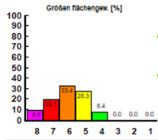
\includegraphics[width=116.3pt,height=104.47pt]{pics/measure_1}};
	%Shape: Circle [id:dp728673139479594] 
	\draw  [color={rgb, 255:red, 126; green, 211; blue, 33 }  ,draw opacity=1 ][fill={rgb, 255:red, 126; green, 211; blue, 33 }  ,fill opacity=1 ] (219,46) .. controls (219,38.82) and (224.82,33) .. (232,33) .. controls (239.18,33) and (245,38.82) .. (245,46) .. controls (245,53.18) and (239.18,59) .. (232,59) .. controls (224.82,59) and (219,53.18) .. (219,46) -- cycle ;
	%Image [id:dp55818248258904] 
	\draw (565.53,154.36) node  {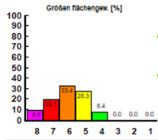
\includegraphics[width=116.3pt,height=104.47pt]{pics/measure_1}};
	%Shape: Circle [id:dp678145460257517] 
	\draw  [color={rgb, 255:red, 126; green, 211; blue, 33 }  ,draw opacity=1 ][fill={rgb, 255:red, 126; green, 211; blue, 33 }  ,fill opacity=1 ] (551,46) .. controls (551,38.82) and (556.82,33) .. (564,33) .. controls (571.18,33) and (577,38.82) .. (577,46) .. controls (577,53.18) and (571.18,59) .. (564,59) .. controls (556.82,59) and (551,53.18) .. (551,46) -- cycle ;
	%Shape: Rectangle [id:dp8368148107013256] 
	\draw  [color={rgb, 255:red, 248; green, 231; blue, 28 }  ,draw opacity=1 ][fill={rgb, 255:red, 248; green, 231; blue, 28 }  ,fill opacity=1 ][line width=0.75]  (348,120) -- (443,120) -- (443,160) -- (348,160) -- cycle ;
	%Shape: Circle [id:dp1828429723656111] 
	\draw  [color={rgb, 255:red, 126; green, 211; blue, 33 }  ,draw opacity=1 ][fill={rgb, 255:red, 126; green, 211; blue, 33 }  ,fill opacity=1 ] (382,94) .. controls (382,86.82) and (387.82,81) .. (395,81) .. controls (402.18,81) and (408,86.82) .. (408,94) .. controls (408,101.18) and (402.18,107) .. (395,107) .. controls (387.82,107) and (382,101.18) .. (382,94) -- cycle ;
	%Shape: Rectangle [id:dp6879768109790683] 
	\draw  [color={rgb, 255:red, 248; green, 231; blue, 28 }  ,draw opacity=1 ][fill={rgb, 255:red, 248; green, 231; blue, 28 }  ,fill opacity=1 ] (294,254) -- (499,254) -- (499,305) -- (294,305) -- cycle ;
	%Bend Up Arrow [id:dp5130011350568686] 
	\draw  [color={rgb, 255:red, 126; green, 211; blue, 33 }  ,draw opacity=1 ][fill={rgb, 255:red, 126; green, 211; blue, 33 }  ,fill opacity=1 ] (240,236) -- (240,269) -- (258,269) -- (258,260) -- (282,278) -- (258,296) -- (258,287) -- (222,287) -- (222,236) -- cycle ;
	%Bend Up Arrow [id:dp5493434724310982] 
	\draw  [color={rgb, 255:red, 126; green, 211; blue, 33 }  ,draw opacity=1 ][fill={rgb, 255:red, 126; green, 211; blue, 33 }  ,fill opacity=1 ] (562.7,235) -- (562.7,268.55) -- (536.4,268.55) -- (536.4,259.4) -- (512,277.7) -- (536.4,296) -- (536.4,286.85) -- (581,286.85) -- (581,235) -- cycle ;
	%Shape: Circle [id:dp4252487137635921] 
	\draw  [color={rgb, 255:red, 126; green, 211; blue, 33 }  ,draw opacity=1 ][fill={rgb, 255:red, 126; green, 211; blue, 33 }  ,fill opacity=1 ] (384,227) .. controls (384,219.82) and (389.82,214) .. (397,214) .. controls (404.18,214) and (410,219.82) .. (410,227) .. controls (410,234.18) and (404.18,240) .. (397,240) .. controls (389.82,240) and (384,234.18) .. (384,227) -- cycle ;
	%Chevron Arrow [id:dp36704668199013146] 
	\draw  [color={rgb, 255:red, 126; green, 211; blue, 33 }  ,draw opacity=1 ][fill={rgb, 255:red, 126; green, 211; blue, 33 }  ,fill opacity=1 ] (118,120) -- (135.4,120) -- (147,140) -- (135.4,160) -- (118,160) -- (129.6,140) -- cycle ;
	%Chevron Arrow [id:dp38485139245994215] 
	\draw  [color={rgb, 255:red, 126; green, 211; blue, 33 }  ,draw opacity=1 ][fill={rgb, 255:red, 126; green, 211; blue, 33 }  ,fill opacity=1 ] (307,120) -- (324.4,120) -- (336,140) -- (324.4,160) -- (307,160) -- (318.6,140) -- cycle ;
	%Chevron Arrow [id:dp7077292276832701] 
	\draw  [color={rgb, 255:red, 126; green, 211; blue, 33 }  ,draw opacity=1 ][fill={rgb, 255:red, 126; green, 211; blue, 33 }  ,fill opacity=1 ] (451,120) -- (468.4,120) -- (480,140) -- (468.4,160) -- (451,160) -- (462.6,140) -- cycle ;
	
	% Text Node
	\draw (21.07,149.37) node [anchor=north west][inner sep=0.75pt]  [color={rgb, 255:red, 255; green, 255; blue, 255 }  ,opacity=1 ] [align=left] {\begin{minipage}[lt]{33.93pt}\setlength\topsep{0pt}
			\begin{center}
				19.488\\Bilder
			\end{center}
			
	\end{minipage}};
	% Text Node
	\draw (355,128) node [anchor=north west][inner sep=0.75pt]  [font=\scriptsize,color={rgb, 255:red, 74; green, 74; blue, 74 }  ,opacity=1 ] [align=left] {\begin{minipage}[lt]{54.7pt}\setlength\topsep{0pt}
			\begin{center}
				\textbf{Transformation}\\ $\displaystyle \to 0,5\ \nicefrac{\mu m}{\text{Pixel}}$
			\end{center}
			
	\end{minipage}};
	% Text Node
	\draw (511.27,68.52) node [anchor=north west][inner sep=0.75pt]   [align=left] {\textbf{{\scriptsize Messung mit AMGuss}}};
	% Text Node
	\draw (559,41) node [anchor=north west][inner sep=0.75pt]  [color={rgb, 255:red, 74; green, 74; blue, 74 }  ,opacity=1 ] [align=left] {\textbf{3}};
	% Text Node
	\draw (390,89) node [anchor=north west][inner sep=0.75pt]  [color={rgb, 255:red, 74; green, 74; blue, 74 }  ,opacity=1 ] [align=left] {\textbf{2}};
	% Text Node
	\draw (179.27,68.52) node [anchor=north west][inner sep=0.75pt]   [align=left] {\textbf{{\scriptsize Messung mit AMGuss}}};
	% Text Node
	\draw (227,41) node [anchor=north west][inner sep=0.75pt]  [color={rgb, 255:red, 74; green, 74; blue, 74 }  ,opacity=1 ] [align=left] {\textbf{1}};
	% Text Node
	\draw (391,222) node [anchor=north west][inner sep=0.75pt]  [color={rgb, 255:red, 74; green, 74; blue, 74 }  ,opacity=1 ] [align=left] {\textbf{4}};
	% Text Node
	\draw (304,265) node [anchor=north west][inner sep=0.75pt]  [color={rgb, 255:red, 74; green, 74; blue, 74 }  ,opacity=1 ] [align=left] {\begin{minipage}[lt]{134.83pt}\setlength\topsep{0pt}
			\begin{center}
				Bestimmung der Abweichung\\\textbf{= Zielwert}
			\end{center}
			
	\end{minipage}};
	\end{tikzpicture}
	\caption{Schematische Darstellung des Modells zur Versuchsdurchführung}
	\label{fig:Versuchsdurchführung}
\end{figure}


\chapter{Umsetzung}
\label{ch:Umsetzung}

Dieses Kapitel beschäftigt sich mit der Umsetzung, also dem Teil der vorliegenden Arbeit bei dem es darum ging, die Aufgabe, nämlich insgesamt 12.992 Lamellengraphit-Messungen mit der Software AMGuss zur Datengenerierung, sowie 232 statistische Versuchsplanungen mir der Minitab (einer Statistik-Software) durchzuführen, umzusetzen. Da eine manuelle Durchführung der Messungen jeden zeitlichen Rahmen gesprengt hätte, wurde dieser Prozess weitestgehend automatisiert.
\\\\
\noindent Für die Implementierung wurde die Skriptsprache Python gewählt, da diese auch die Möglichkeit bietet, einen objektorientierten Programmierstil umzusetzen. Darüber hinaus war es durch die Einbindung der Bibliothek PyAutoIt möglich, die gesamte Funktionalität von AutoIt (siehe auch Abschnitt \ref{sec:UeberblickAutoIt} auf Seite \pageref{sec:UeberblickAutoIt}) verfügbar und nutzbar zu machen. Dadurch konnte die Automatisierung der durchzuführenden Messungen in Verbindung mit einem objektorientierten Programmierstil sehr gut umgesetzt werden.
\\\\
\noindent Nach einer Darstellung der Komponentenstruktur als Überblick über die Implementierung, folgt dann in weiteren Abschnitten die Beschreibung der zu Implementierenden Funktionalität anhand von Aktivitätsdiagrammen und schließlich die Klassendiagramme die zeigen, wie die Objektorientierung dabei geholfen hat, das die einzelnen Aufgaben in Teilaufgaben zerlegt und separat durchgeführt werden konnten.

\newpage

\section{Darstellung der Komponenten}
\label{sec:Komponentendarstellung}

Wie bereits angedeutet, wurde die Gesamtaufgabe auf verschiedene, aufeinander aufbauende Arbeitsschritte aufgeteilt. Diese Komponenten erzeugen Daten, speichern diese in einer dafür implementierten Datenstruktur, die dann schließlich serialisiert, gespeichert und so für die Nutzung weitere Komponenten verfügbar gemacht wird. Abbildung xyz zeigt die einzelnen Bestandteile wobei anzumerken ist, das diese nicht, wie im herkömmlichen Sinne der objektorientierten Programmierung über implementierte Schnittstellen verbunden sind. Vielmehr handelt es sich um völlig getrennte Funktionseinheiten. Die Pfeil-Konnektoren, welche die Komponenten miteinander verbinden, symbolisieren also Abhängigkeitsbeziehungen in dem Sinne, das die Komponente auf welche die Pfeilspitze zeigt auf die Ergebnisse derjenigen am anderen Endes des Pfeils voraussetzt.

\begin{figure}[H]
	\centering
	\boxed{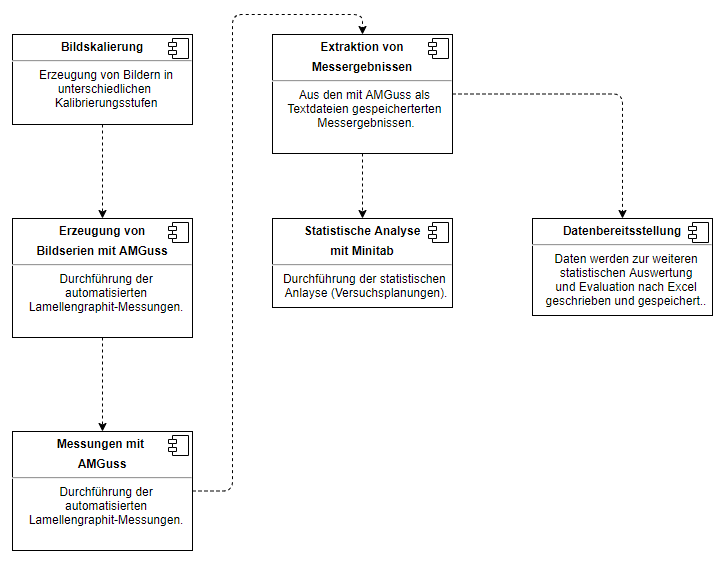
\includegraphics[scale=0.8]{pics/components}}
	\caption{Darstellung der Systemkomponenten und Abhängigkeiten}
	\label{fig:Komponentendiagramm}
\end{figure}



\section{Aktivitätsdiagramme}

\label{sec:Workflows}
Aktivitätsdiagramme sind Teil von UML (Unifiend Modelling Language) zur Modellierung von Software-Systemen und ein geeignetes Werkzeug, die Kontroll- und Datenflüsse der für diese Arbeit entwickelten Skript-Bibliothek anschaulich darzustellen. Dadurch werden die zu entwickelnden funktionalen Abläufe eindeutig spezifiziert - und zwar unabhängig davon, wie dies später programmatisch und algorithmisch umgesetzt wird. In den folgenden Unterabschnitten werden nun, nach unterschiedlichen Funktionseinheiten gegliedert, diese anhand von Aktivitätsdiagrammen eindeutig beschrieben, um so dem Leser zunächst einen Überblick über die funktionalen Zusammenhänge zu geben. Die Reihenfolge der Darstellung folgt dabei den dargestellten Abhängigkeiten im Komponentendiagramm.

\subsection{Bildskalierung in unterschiedliche Kalibrierungsstufen}

Die Erzeugung von Bildern in unterschiedlichen Kalibrierungsstufen entspricht der im Abschnitt \ref{sec:ErzeugungVonBildern} auf Seite \pageref{sec:ErzeugungVonBildern} bereits eingehend beschriebenen Vorgehensweise.

\subsection{Erstellung einer Bildserie mit AMGuss}
\label{subsec:FlowErstellungBildserieAMGuss}

Um eine Lamellenguss-Auswertung mit der Software AMGuss durchzuführen, sollte für jedes zu messende Bild eine sog. Bildserie vorliegen. Es können grundsätzlich auch Serien mit mehreren Bildern erstellt und auf einmal gemessen werden, jedoch hat sich dies nach Durchführung mehrerer Versuche im vorliegenden Kontext als nicht zweckmäßig erwiesen. Daher wurde für jedes zu messende Bild eine eigene Bildserie erstellt
\\\\
\noindent Der funktionale Ablauf dabei ist in der folgenden Abbildung \ref{fig:FlowBildserieErstellen} dargestellt.


\begin{figure}[H]
	\centering
	\boxed{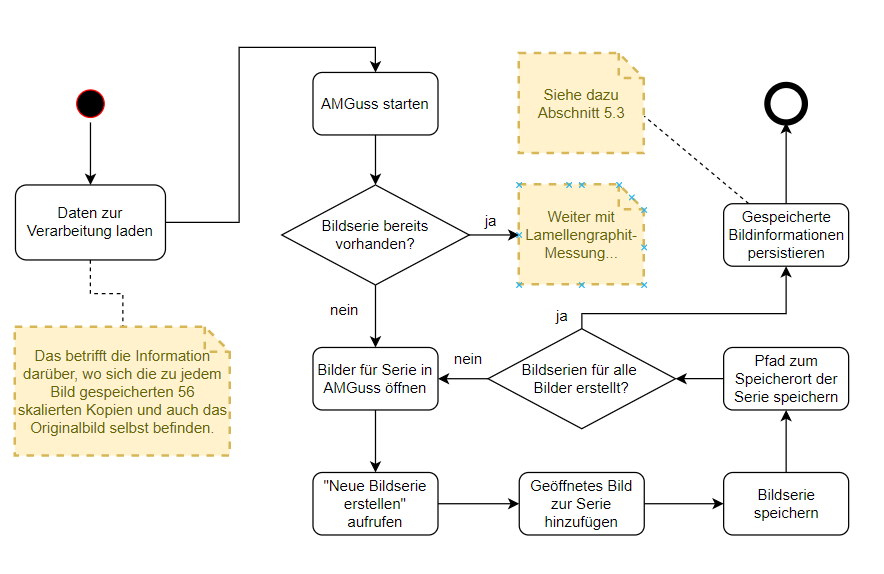
\includegraphics[scale=0.8]{pics/flow_create_picture_set_amguss}}
	\caption{Aktivitätsdiagramm zur Erstellung einer Bildserie mit AMGuss}
	\label{fig:FlowBildserieErstellen}
\end{figure}

\noindent Im Ergebnis wird dadurch von AMGuss eine Textdatei.cia erzeugt, welche Informationen über das Bild, also den Pfad zum Speicherort und ggf. noch weitere Bildinformationen enthält. Den Inhalt der erzeugten Datei zeigt die nachstehende Abbildung \ref{fig:CiaContent}.

\begin{figure}[H]
	\centering
	\boxed{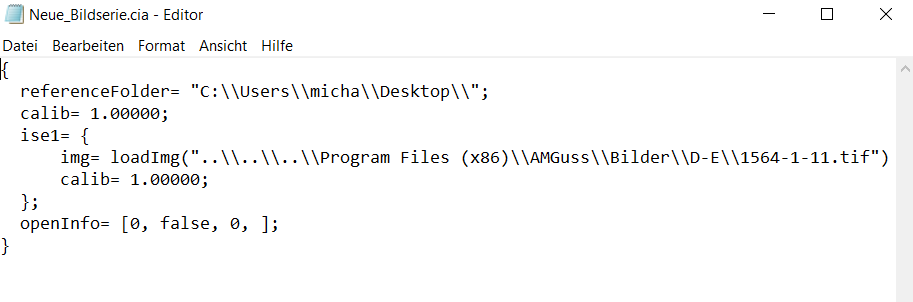
\includegraphics[scale=0.45]{pics/CiaContent}}
	\caption{Inhalt einer .cia-Datei für eine Bildserie}
	\label{fig:CiaContent}
\end{figure}

\noindent Am Ende wird die erzeugte cia-Datei gespeichert, sowie auch der Pfad zum Speicherort, so das bei späteren Verwendung darauf zugegriffen werden kann.

\subsection{Durchführung einer Lamellengraphit-Messung mit AMGuss}
\label{subsec:FlowLamellengussmessung}

\begin{figure}[H]
	\centering
	\boxed{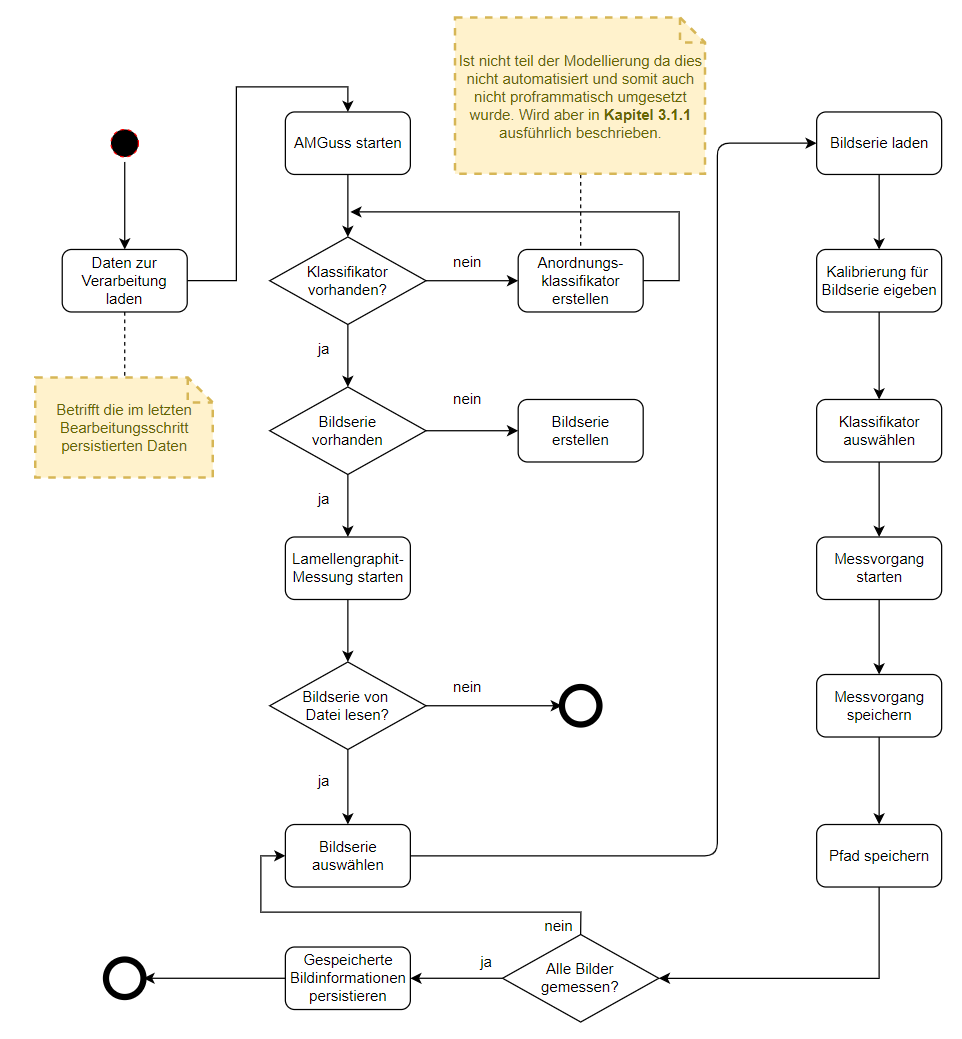
\includegraphics[scale=0.8]{pics/flow_lamellar_graphite_evaluation}}
	\caption{Aktivitätsdiagramm zur Durchführung einer Lamellengraphit-Messung mit AMGuss}
	\label{fig:FlowLamellengussMessung}
\end{figure}

\section{Extraktion der Messergebnisse aus den mit AMGuss gespeicherten Messungen}

\section{Durchführung der statistischen Analyse mit Minitab}

\section{Datenbereitstellung in Excel}



\chapter{Evaluation}
\label{ch:Evaluation}

\section{Auswertung der Analysedaten}
\label{sec:AuswertungAnalysedaten}

\subsection{Auswertung der statistischen Versuchsplanung}
\label{subsubsec:AuswertungStatVpl}
Wie in Kapitel \ref{sec:StatVersPlanung} ab Seite \pageref{sec:StatVersPlanung} bereits beschrieben, dient die statistische Versuchsplanung dazu sichtbar zu machen, welchen Einfluss die die unterschiedlichen Faktoren (Steuer- und Störgrößen) auf den Zielwert (Messfehler, siehe dazu auch Kapitel \ref{subsec:DefZiel}) haben.Das Ergebnis zeigt die nachstehende Abbildung \ref{fig:DAPareto} sowie Tabelle \ref{tab:DAPareto}, in der die für das Diagramm berechneten Werte tabellarisch dargestellt werden. 

\begin{figure}[H]
	\centering
	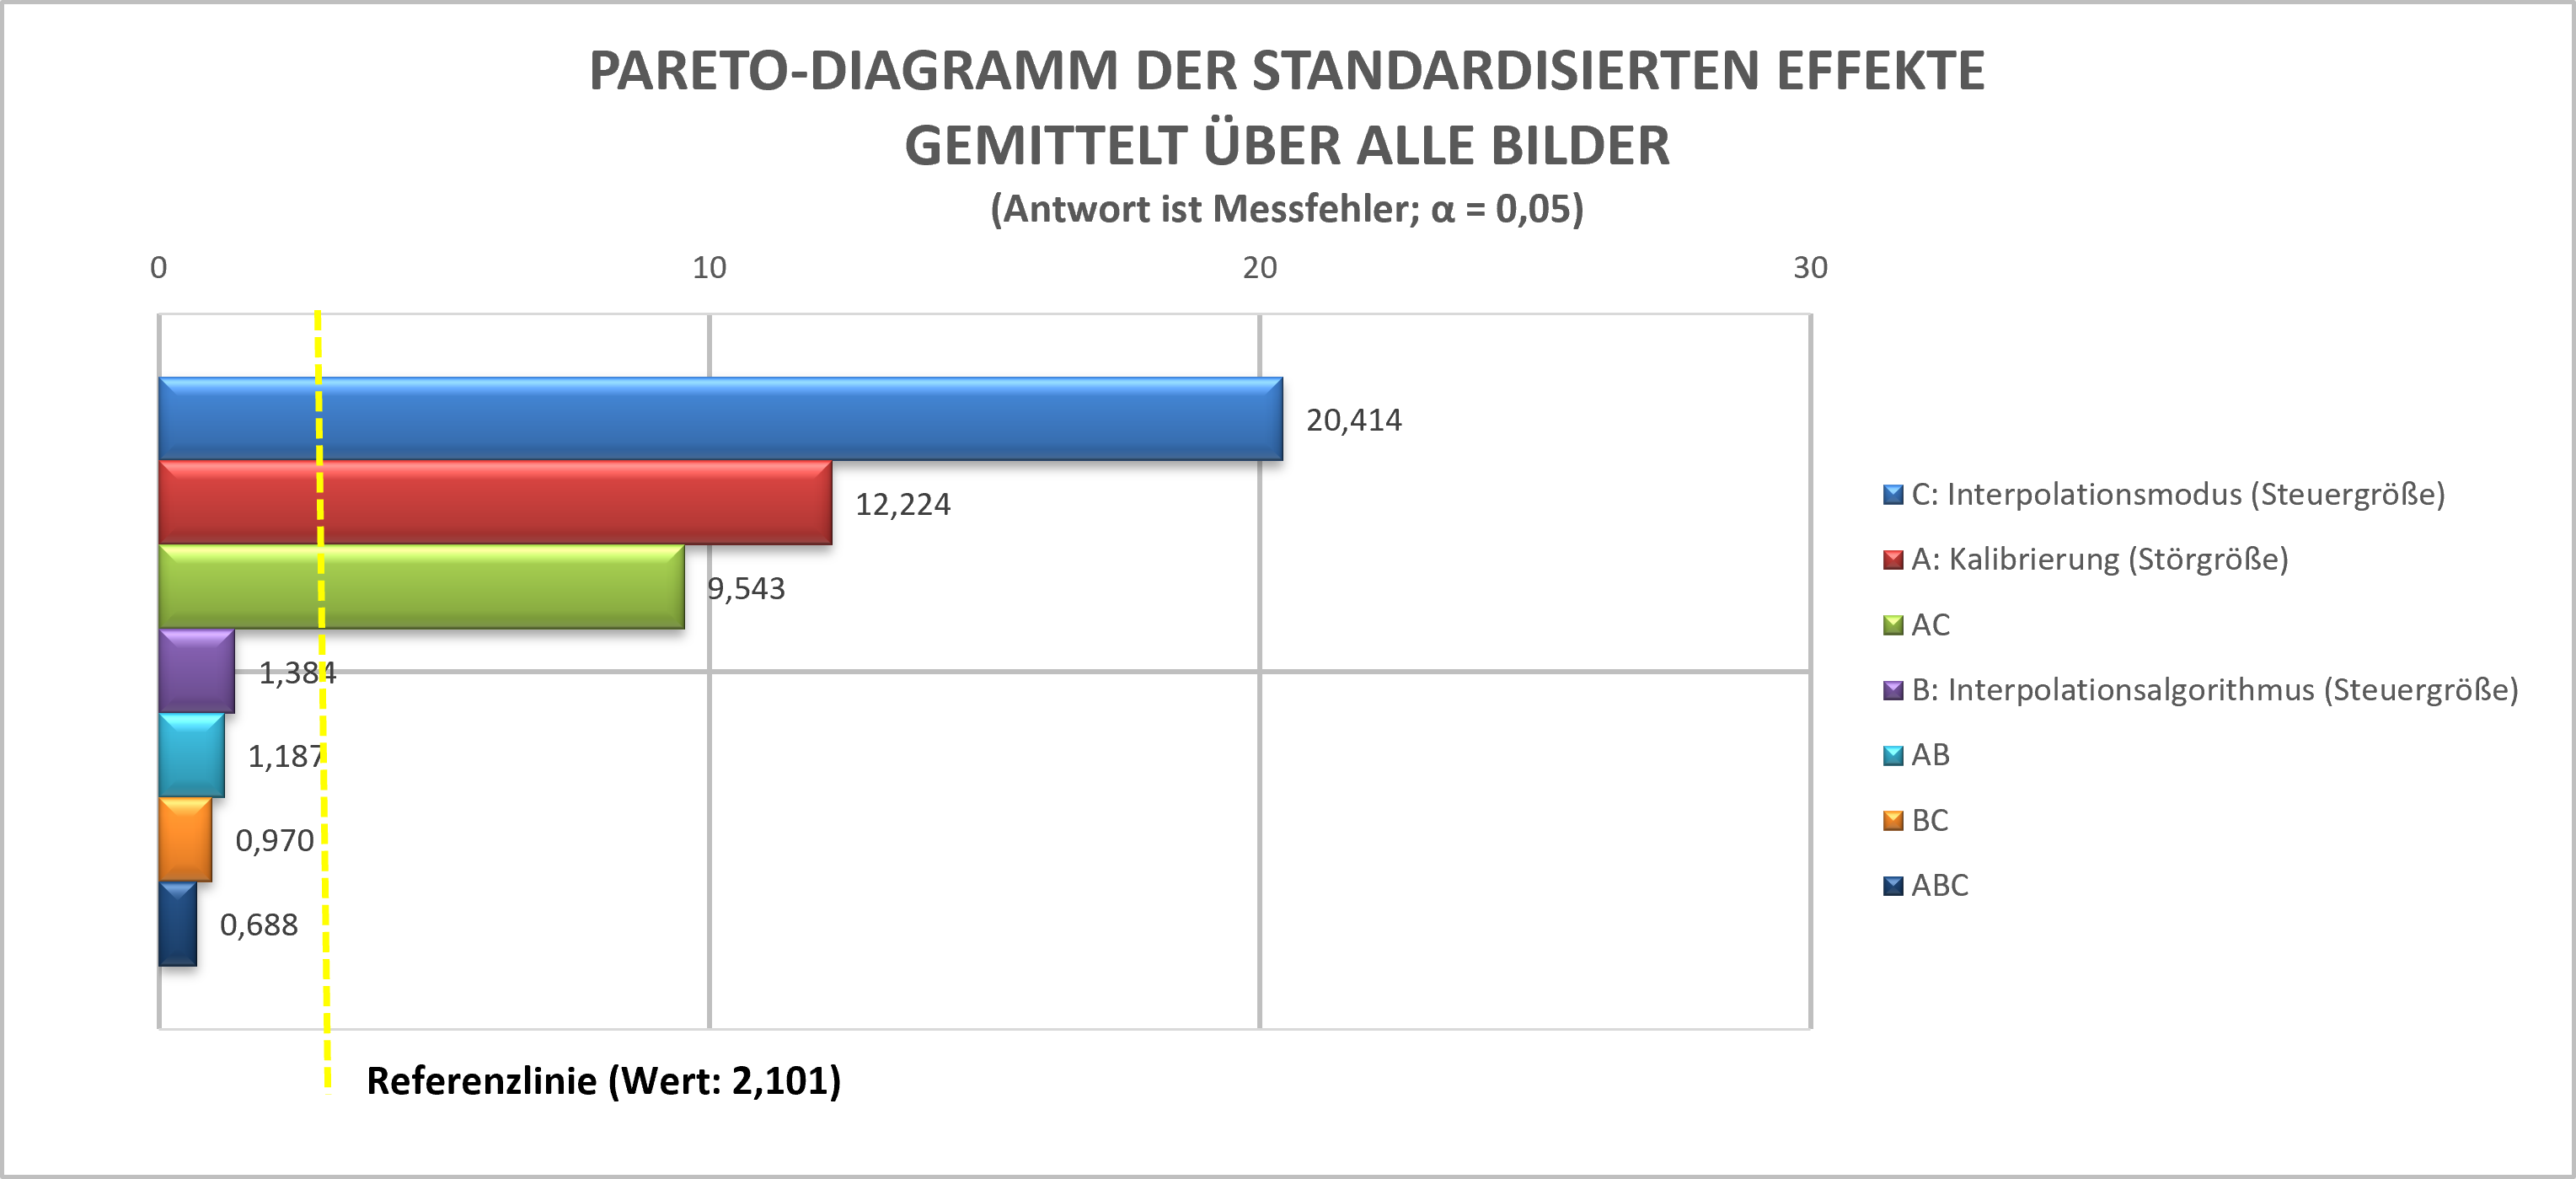
\includegraphics[width=14cm, height=\textheight, keepaspectratio]{pics/DA_Pareto}
	\caption{Pareto-Diagramm der standardisierten Effekte}
	\label{fig:DAPareto}
\end{figure}

\begin{table}[H]
	\caption{Berechnete Mittelwerte (über alle Bilder) zum Pareto-Diagramm der standardisierten Effekte}
	\begin{figure}[H]
		\centering
		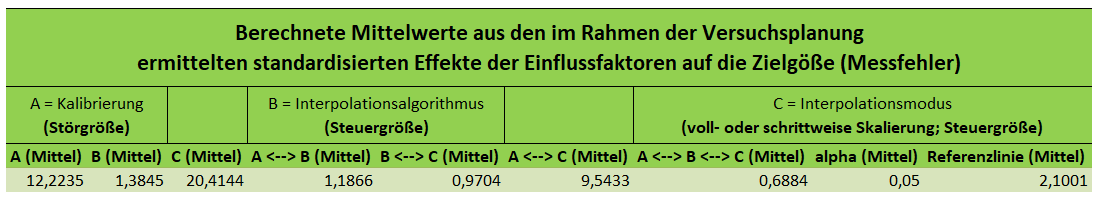
\includegraphics[width=\textwidth,height=\textheight,keepaspectratio]{pics/Tab_DA_Pareto}
		\label{tab:DAPareto}
	\end{figure}
\end{table}

\noindent Das Diagramm zeigt die Absolutwerte der standardisierten Effekte, geordnet vom größten zum kleinsten. Ein wichtiger Indikator ist die dargestellte Referenzlinie. Nach \cite{minitab_pareto} ist Methode, die Minitab zum Zeichnen des Pareto-Diagramms der Effekte verwendet, abhängig von den Freiheitsgraden für den Fehlerterm. Wenn dieser einen oder mehrere Freiheitsgrade hat, wird die gelbe Linie im Pareto-Diagramm bei t gezeichnet, wobei $t$ das $1-\nicefrac{\alpha}{2}$ - Quantil einer t-Verteilung mit Freiheitsgraden gleich den Graden von Freiheit für den Fehlerterm ist. Minitab bezeichnet dieses Diagramm als Pareto-Diagramm der standardisierten Effekte. Wenn der Fehlerterm null Freiheitsgrade hat, identifiziert Minitab wichtige Effekte mithilfe des Lenth-Pseudostandardfehlers (PSE). Die rote Linie des Pareto-Diagramms wird dann an der Fehlergrenze gezeichnet, die wie folgt lautet:

\begin{equation}
	ME = t\cdot PSE
\end{equation}

\noindent Faktoren die diese Linie überschreiten gelten als statistisch signifikant. 
\\\\
Wie in Kapitel \ref{ch:Umsetzung} bereits beschrieben wurden Versuchsplanungen für alle 232 Probebilder separat durchgeführt. Um die im Diagramm dargestellten Werte zu berechnen wurde die Werte aller Einzel-Pareto-Diagramme aufsummiert, durch die Anzahl der Bilder geteilt und auf dieser Grundlage ein Pareto-Diagramm der standardisierten Effekte zu erstellen, welches einen Querschnitt über  alle Probebilder liefert.
\\\\
\noindent Vor diesem Hintergrund kann also geschlossen werden, dass die Einflussfaktoren \textbf{Interpolationsmodus} und \textbf{Kalibrierung} sowie die Wechselwirkung beider Faktoren insgesamt betrachtet den größten Einfluss auf die Zielgröße haben.
\\\\
\noindent Wenngleich das Pareto-Diagramm dadurch wichtige Hinweise zum Verständnis der Daten liefert und die Haupteffekte sichtbar macht, kann damit nicht festgestellt werden, durch welche Effekte den Wert der Antwortvariablen vergrößert oder verkleinert wird. Um diese Fragestellung zu beantworten, wurden weitere Analysen durchgeführt, die im folgenden beschrieben und ausgewertet werden.


\subsection{Analyse der eingesetzten Interpolationsverfahren}

Wie im vorigen Abschnitt schon angedeutet geht es in diesem vor allem darum herauszufinden, wie genau sich die bereits identifizierten Haupteffekte auf die durch Skalierung der Bilder induzierten Messfehler auswirken. Da sich der gesamte Messfehler aus unterschiedlichen Messfehlerkategorien zusammensetzt wird dieser nun, nach einer vorausgehenden Gesamtbetrachtung in seine einzelnen Komponenten zerlegt und diese u.a. mit Methoden der deskriptiven Statistik näher untersucht. Ausgehend von der Gesamtbetrachtung ist es so möglich Schritt für Schritt ein tieferes Verständnis über die Wirkungsweise der unterschiedlichen Einflussgrößen (insbesondere der Interpolationsalgorithmen) auf die Zielgröße zu gewinnen.

\subsubsection{Gesamtfehlerbetrachtung}
\label{subsubsec:AuswertungGesamtfehlerbetrachtung}
 In Abschnitt \ref{fig:DAPareto} wurde der \textbf{Interpolationsmodus} als Haupteffekt mit dem größten Einfluss auf die Zielvariable identifiziert. Wie jedoch die folgende Abbildung \ref{fig:DAGesamtAbsolut_Alle} in Verbindung mit Tabelle \ref{tab:DAGesamtAbsolutAlle} zeigt, hat diese Einflussgröße zwar ohne Zweifel den größten Effekt, jedoch nicht in die gewünschte Richtung da es ja darum geht den Messfehler zu minimieren. 

\begin{figure}[H]
	\centering
	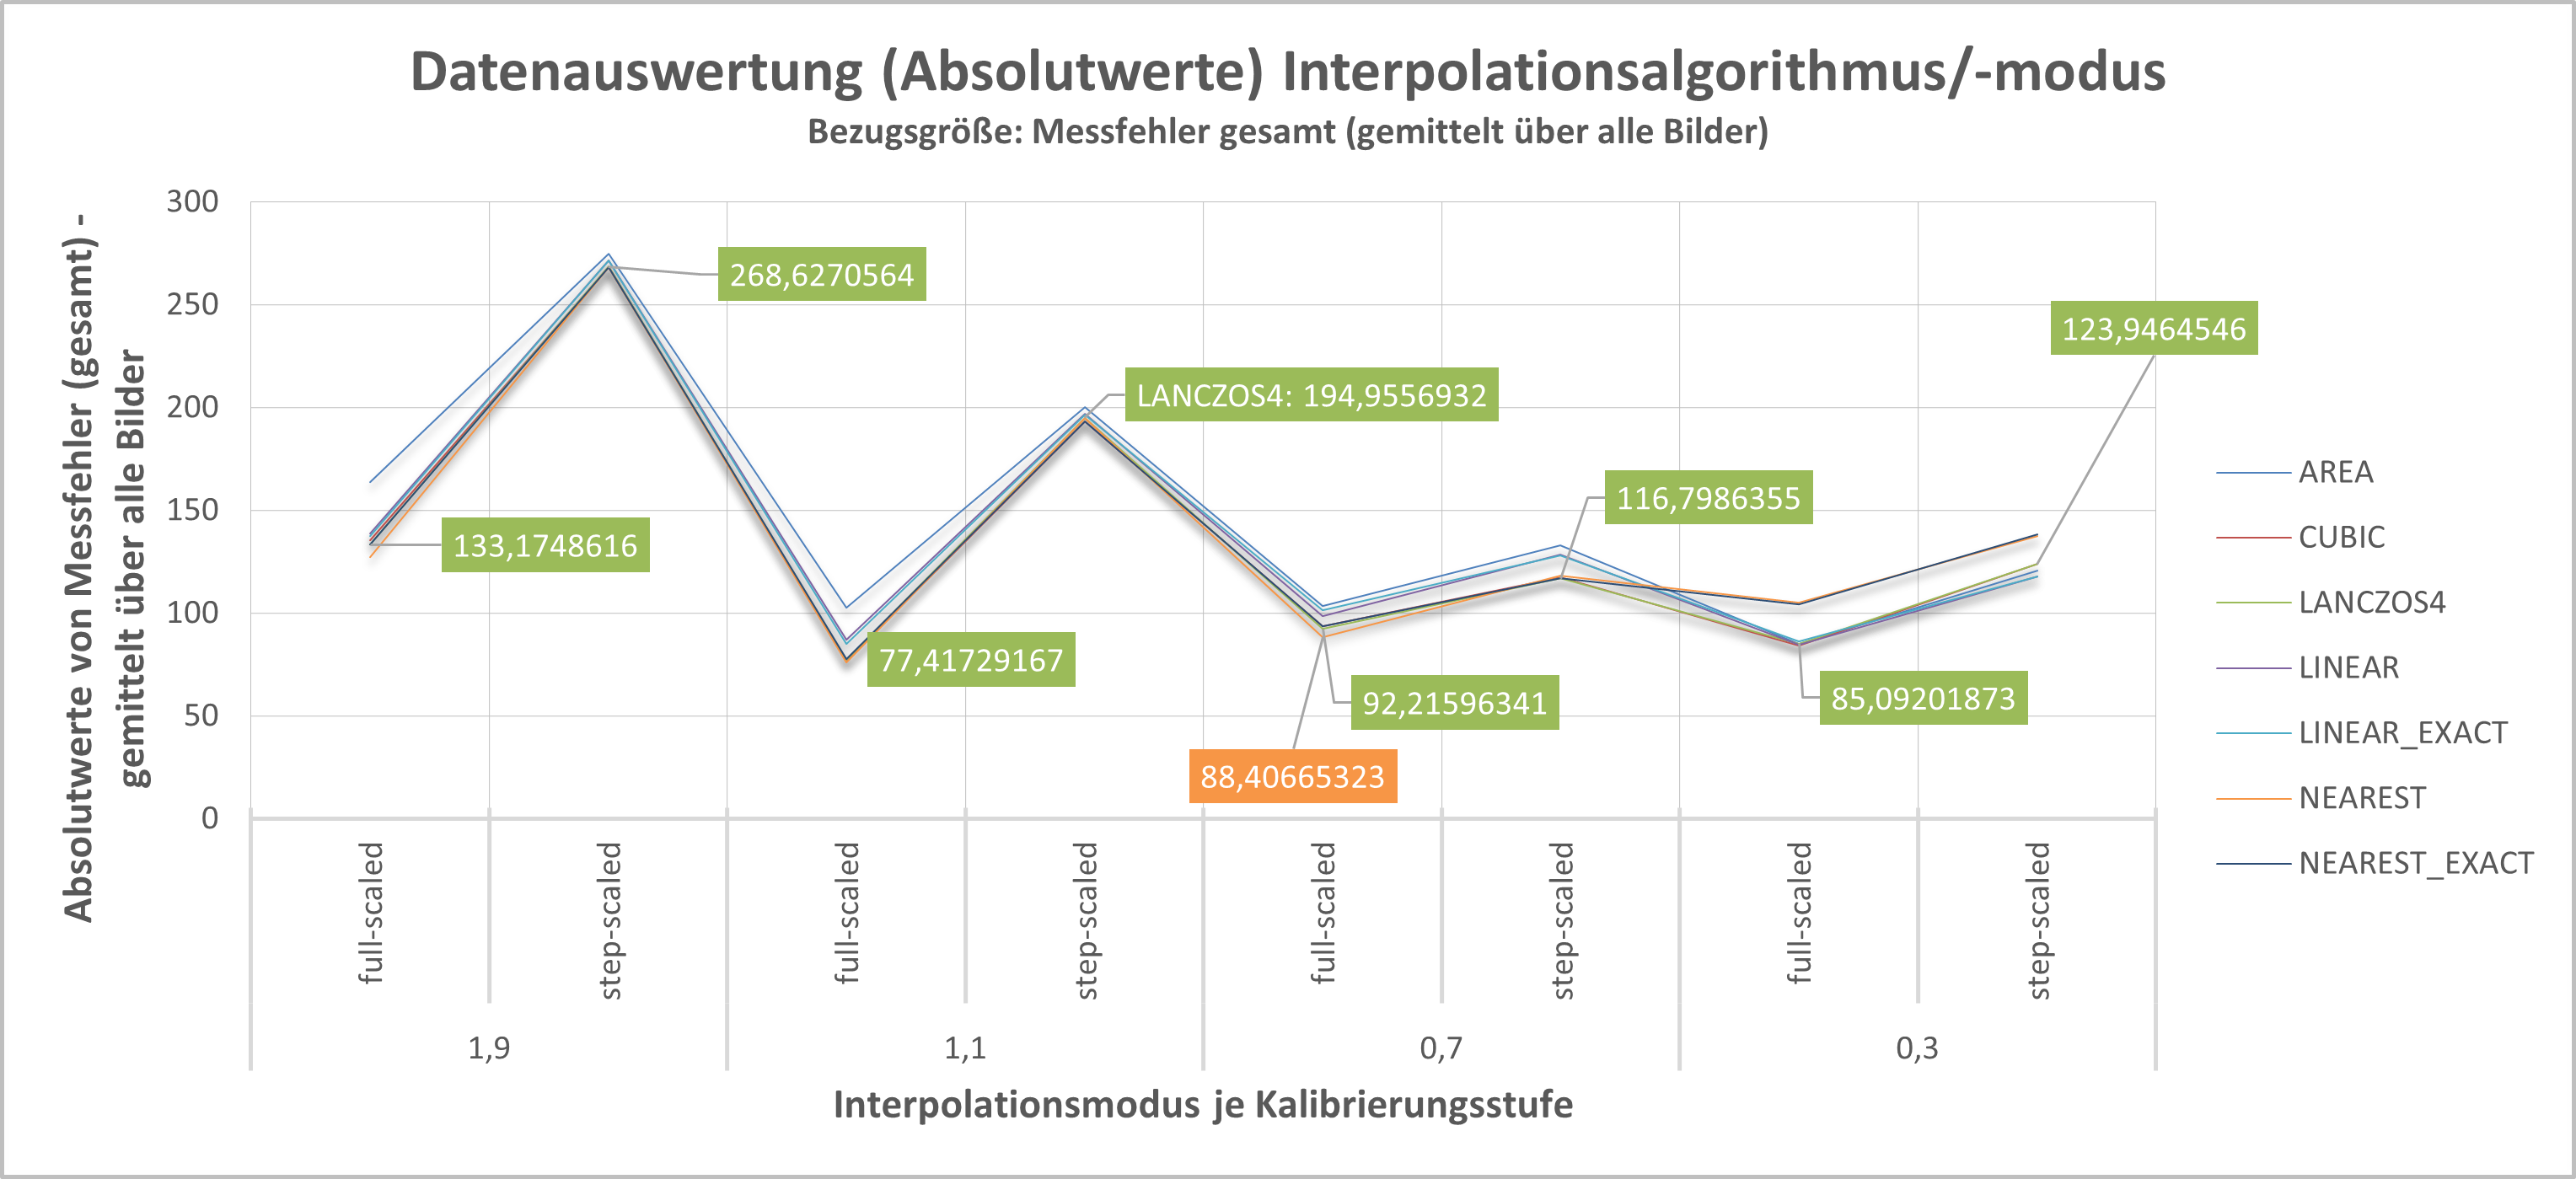
\includegraphics[width=11cm, height=\textheight, keepaspectratio]{pics/DA_Gesamt_Absolut_Alle}
	\caption{Auswertung des Messfehlers (Gesamt)}
	\label{fig:DAGesamtAbsolut_Alle}
\end{figure}
	
\begin{table}[H]
	\centering
	\caption{Daten zur Auswertung des Messfehlers (Gesamt)}
	\label{tab:DAGesamtAbsolutAlle}
	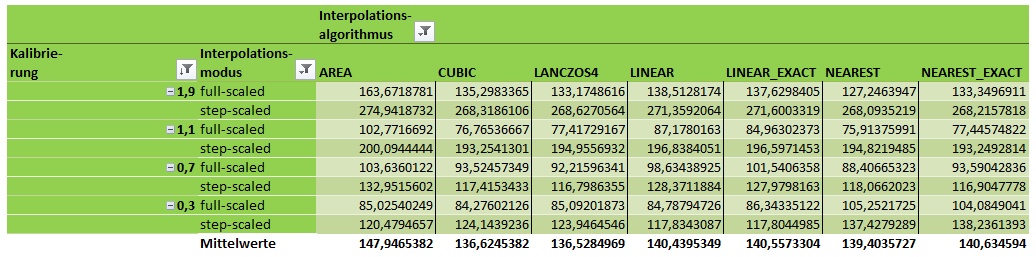
\includegraphics[width=\textwidth,height=\textheight,keepaspectratio]{pics/Tab_DA_Gesamt_Absolut_Alle}
\end{table}

\noindent An den berechneten Mittelwerten in der Tabelle ist zu erkennen, das LANCZOS4 über alle Kategorien den geringsten durchschnittlichen Fehler erzeugt. Allerdings zeigen die Daten auch, das dies nicht repräsentativ für alle Kalibrierungsstufen ist. Man betrachte z.B. Kalibrierungsstufe 0,7 bei Vollskalierung - in diesem Bereich liegt der Fehlerwert von Nächster-Nachbar mit ca. 88,41 etwa 4 Einheiten unter dem von LANCZOS4 mit ca. 92,22. Darüber hinaus ist zu beobachten, dass der Fehler mit zunehmender Ausgangskalibrierung wächst. Vergleicht man etwa am Beispiel von LANCZOS4 die Werte bei Kalibrierung  0,3  und 1,9 $\nicefrac{\mu m}{\text{Pixel}}$ stellt man fest, das der Messfehlerwert bei 1,9 $\nicefrac{\mu m}{\text{Pixel}}$ um fast 57 $\%$ über dem bei Kalibrierung 0,3 liegt. Dadurch zeigt sich, dass die Vergrößerung von Bildern (also Verringerung der Kalibrierung) wohl offensichtlich weniger gut funktioniert als in die entgegengesetzte Richtung.
\\\\
Betrachtet man dagegen die Streuungsparameter Standardabweichung und Varianz, ergibt sich ein etwas anderes Bild. Während die Standardabweichung über alle Bereiche hinweg sehr niedrig ausfällt und kaum schwankt ist die Varianz, also die Streuung in den Daten wesentlich höher und schwankt im Bereich von ca. 135,62 bei Kalibrierung 0,3 bis ca. 367,18 bei einer Ausgangskalibrierung von 1,9 $\nicefrac{\mu m}{\text{Pixel}}$ (hier am Beispiel von LANCZOS4) ziemlich stark. Ebenfalls ist auffällig, das die kubische Interpolation in den Kalibrierungsbereichen 0,3 und 1,1 $\nicefrac{\mu m}{\text{Pixel}}$ die niedrigste Varianz, also auch im Vergleich zu LANCZOS4 aufweist.  Die nachstehende Abbildung \ref{fig:DAGesamtStreu1Alle} sowie die dazugehörige Datentabelle \ref{tab:DAGesamtStreu1Alle} geben diesen Zusammenhang sehr gut zu erkennen.

\begin{figure}[H]
	\centering
	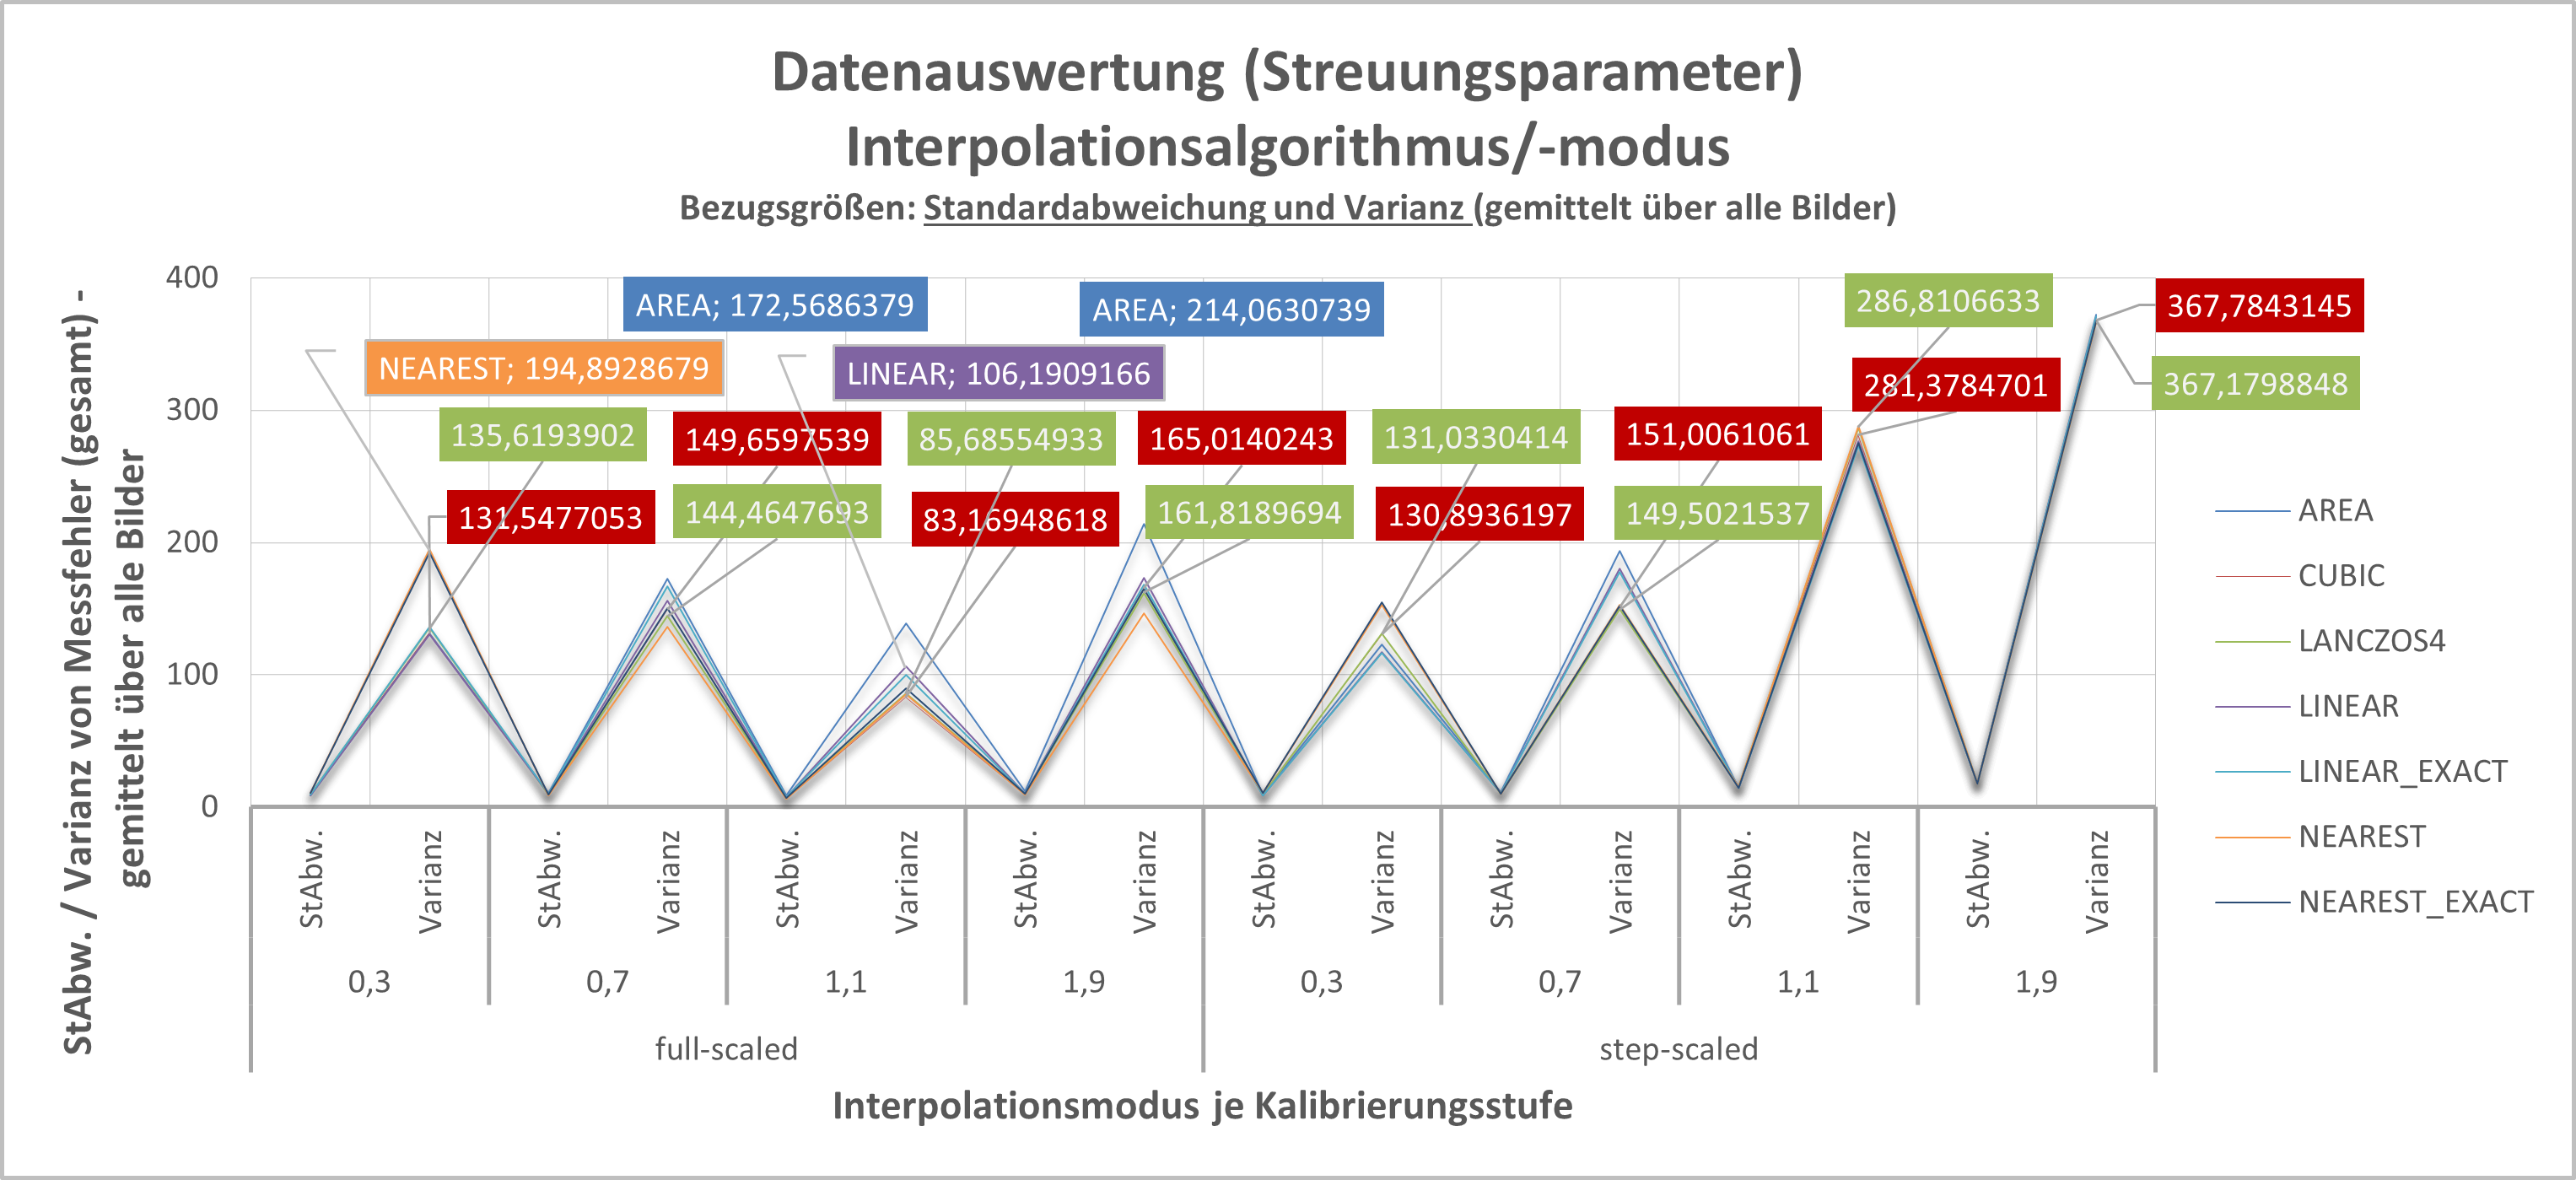
\includegraphics[width=11cm, height=\textheight, keepaspectratio]{pics/DA_Gesamt_Streu1_Alle}
	\caption{Streuungsparameter (Standardabweichung u. Varianz) bezogen\\ auf den gesamten Messfehler}
	\label{fig:DAGesamtStreu1Alle}
\end{figure}
	
\begin{table}[H]
	\centering
	\caption{Daten zu den berechneten Streuungsparametern (Standardabweichung u. Varianz) bezogen auf den gesamten Messfehler}
	\label{tab:DAGesamtStreu1Alle}
	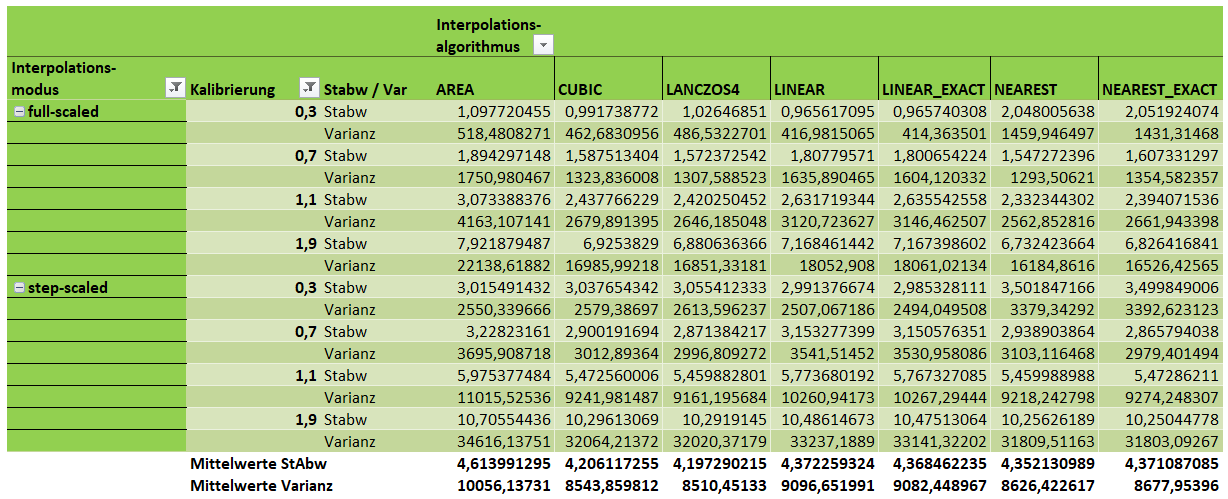
\includegraphics[width=\textwidth,height=\textheight,keepaspectratio]{pics/Tab_DA_Gesamt_Streu1_Alle}
\end{table}

\noindent Hierbei wird deutlich, dass LANCZOS4, wenn auch den geringsten gesamten Messfehler über alle Bereiche, andererseits in einigen Bereichen eine sehr hohe Varianz besitzt (grüne Datenpunkte), was auf eine hohe Streuung hindeutet. Demgegenüber hat die kubische Interpolation über alle Kategorien die geringste Varianz (rote Datenpunkte). Die Frage, welcher Kandidat die höchste Varianz aufweist, kann nicht eindeutig beantwortet werden, da diese sich kategorial unterscheidet. Die entsprechenden Datenpunkte und Werte sind in der Abbildung in der dem entsprechenden Algorithmus jeweils zugeordneten Farbe ebenfalls eingetragen, jedoch nur für die Vollskalierung, um die Grafik nicht zu sehr zu überlagern. 
\\\\
Ein weiteres Streuungsmaß, dass sich zur Beschreibung von Daten sehr gut eignet, ist die Variationsbreite, die zeigt, wie weit die Werte genau streuen. Abbildung \ref{fig:DAGesamtStreu2Alle} i. V. m. Tabelle \ref{tab:DAGesamtStreu2Alle} zeigt diesen Sachverhalt und beschreibt in absoluten Zahlen, wie weit die Messfehlerwerte je Interpolationsalgorithmus, Interpolationsmodi und Stufe der Ausgangskalibrierung streuen. 

\begin{figure}[H]
	\centering
	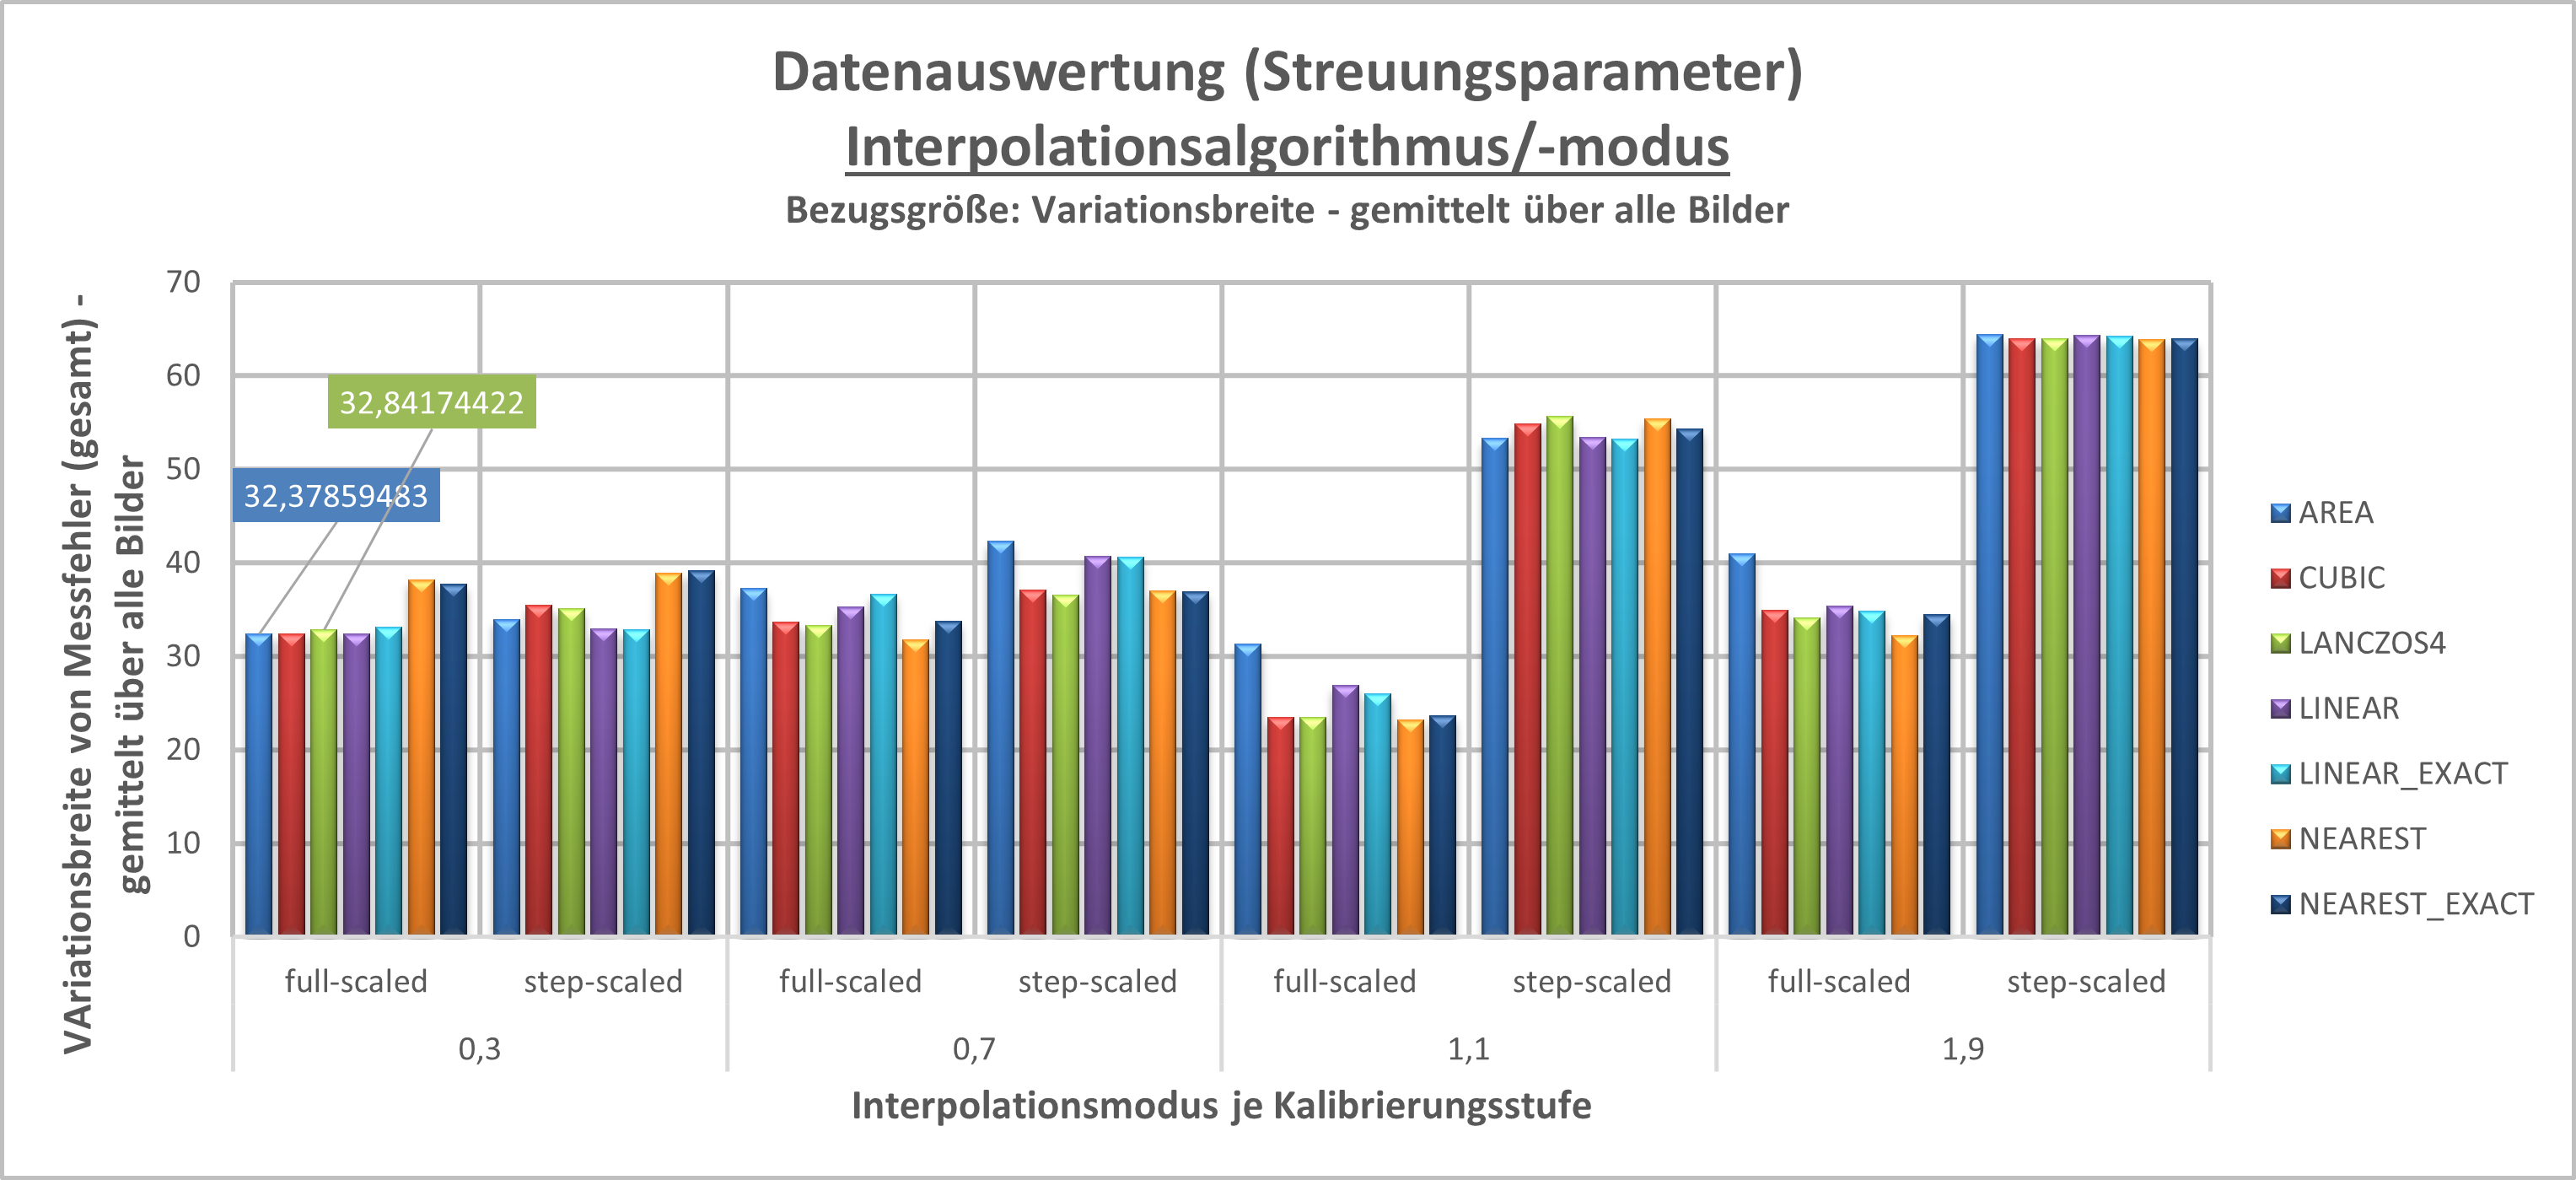
\includegraphics[width=11cm, height=\textheight, keepaspectratio]{pics/DA_Gesamt_Streu2_Alle}
	\caption{Streuungsparameter (Variationsbreite) bezogen auf den gesamten Messfehler}
	\label{fig:DAGesamtStreu2Alle}
\end{figure}

\begin{table}[H]
	\centering
	\caption{Daten zum berechneten Streuungsparameter (Variationsbreite) bezogen auf den gesamten Messfehler}
	\label{tab:DAGesamtStreu2Alle}
	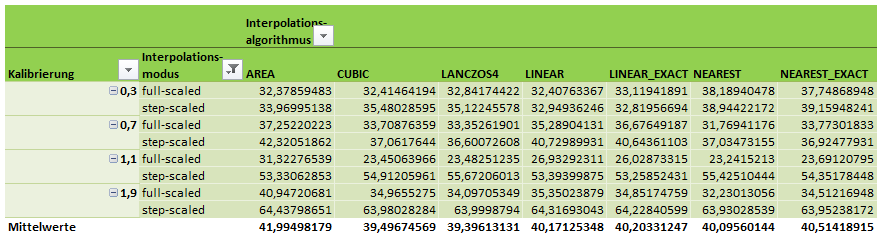
\includegraphics[width=\textwidth, height=\textheight, keepaspectratio]{pics/Tab_DA_Gesamt_Streu2_Alle}
\end{table}


\noindent Wie zu erwarten ist auch die Variationsbreite bei LANCZOS4 am geringsten (bezogen auf den Mittelwert), jedoch nicht in allen Kalibrierungsstufen. Betrachtet man bspw. die Kalibrierungsstufe $0,3~\nicefrac{\mu m}{\text{Pixel}}$ ist zu erkennen, das LANCZOS4 im Vergleich zur flächenbasierten Interpolation einen minimal höhere Variationsbreite der Messfehlerwerte aufweist. 
\\\\
Die Ergebnisse aus diesem Abschnitt lassen sich wie folgt kurz zusammenfassen:
\\\\
\colorbox{gray!10}{
	\label{box:ErgebnisGesamtauswertung}
	\begin{minipage}{0.975\textwidth}
		\textbf{\underline{Ergebnis der Gesamtauswertung:}}\\\\
		Zusammenfassend kann für diesen Abschnitt festgehalten werden, dass die LANCZOS4-Interpolation zwar im Durchschnitt über alle Bereiche den kleinsten Fehler erzeugt. Jedoch allerdings in einigen Bereichen auch eine höhere Streuung aufweist, als die kubische Interpolation, welche zwar die geringste durchschnittliche Varianz besitzt, aber nicht immer den geringsten Fehler erzeugt.
		\\\\
		\noindent Des Weiteren kann festgehalten werden, dass die schrittweise Skalierung tendenziell immer größere Fehler erzeugt, als Voll-Skalierung - sehr wahrscheinlich deshalb, weil sich die Fehler bei der mehrfach-Skalierung addieren. 
		\\\\
		\noindent Eine weitere wichtige Beobachtung ist die, dass die Verkleinerung von Bildern wohl offensichtlich generell besser funktioniert als die Vergrößerung, da in den Daten ein genereller Trend zu erkennen ist, wonach der Fehler bei zunehmender Ausgangskalibrierung stetig wächst.
	\end{minipage}
}
\\\\\\
Da die Gesamtbetrachtung noch keine eindeutige Interpretation zulässt, wird nun im weiteren Verlauf der Analyse der Gesamt-Messfehler in seine Bestandteile zerlegt und zunächst innerhalb der Größenklassen (anzahlgewichtet) genauer untersucht.

\subsubsection{Auswertung nach Größenklassen (anzahlgewichtet)}
\label{subsubsec:AuswertungGKanz}
Die Größenklassen (anzahlgewichtet) entsprechen den Histogramm-Werten, welche durch die Software AMGuss bei der Durchführung einer Lamellengraphitauswertung als Teil des Analyseergebnisses berechnet werden. Durch die getrennte Erfassung der Abweichungen in den Originalbildern ist es nun möglich, diese Fehlerkategorie separat zu untersuchen. Wie im vorherigen Abschnitt bereits geschehen erfolgt auch hier zunächst einer Gesamtbetrachtung über die Gesamte Kategorie (bestehend aus 8 Klassen). Zusätzlich wird die Analyse noch durch eine Einzel-Fehleranalyse bezogen auf die 8 Größenklassen erweitert. Abbildung \ref{fig:DAGesamtAbsolutGKanzahl} und die damit verbundene Datenbasis in Tabelle \ref{tab:DAGesamtAbsolutGKanzahl} vergleichen wieder zunächst die verschiedenen Interpolationsalgorithmen je Interpolationsmodi und Kalibrierungsstufe.

\begin{figure}[H]
	\centering
	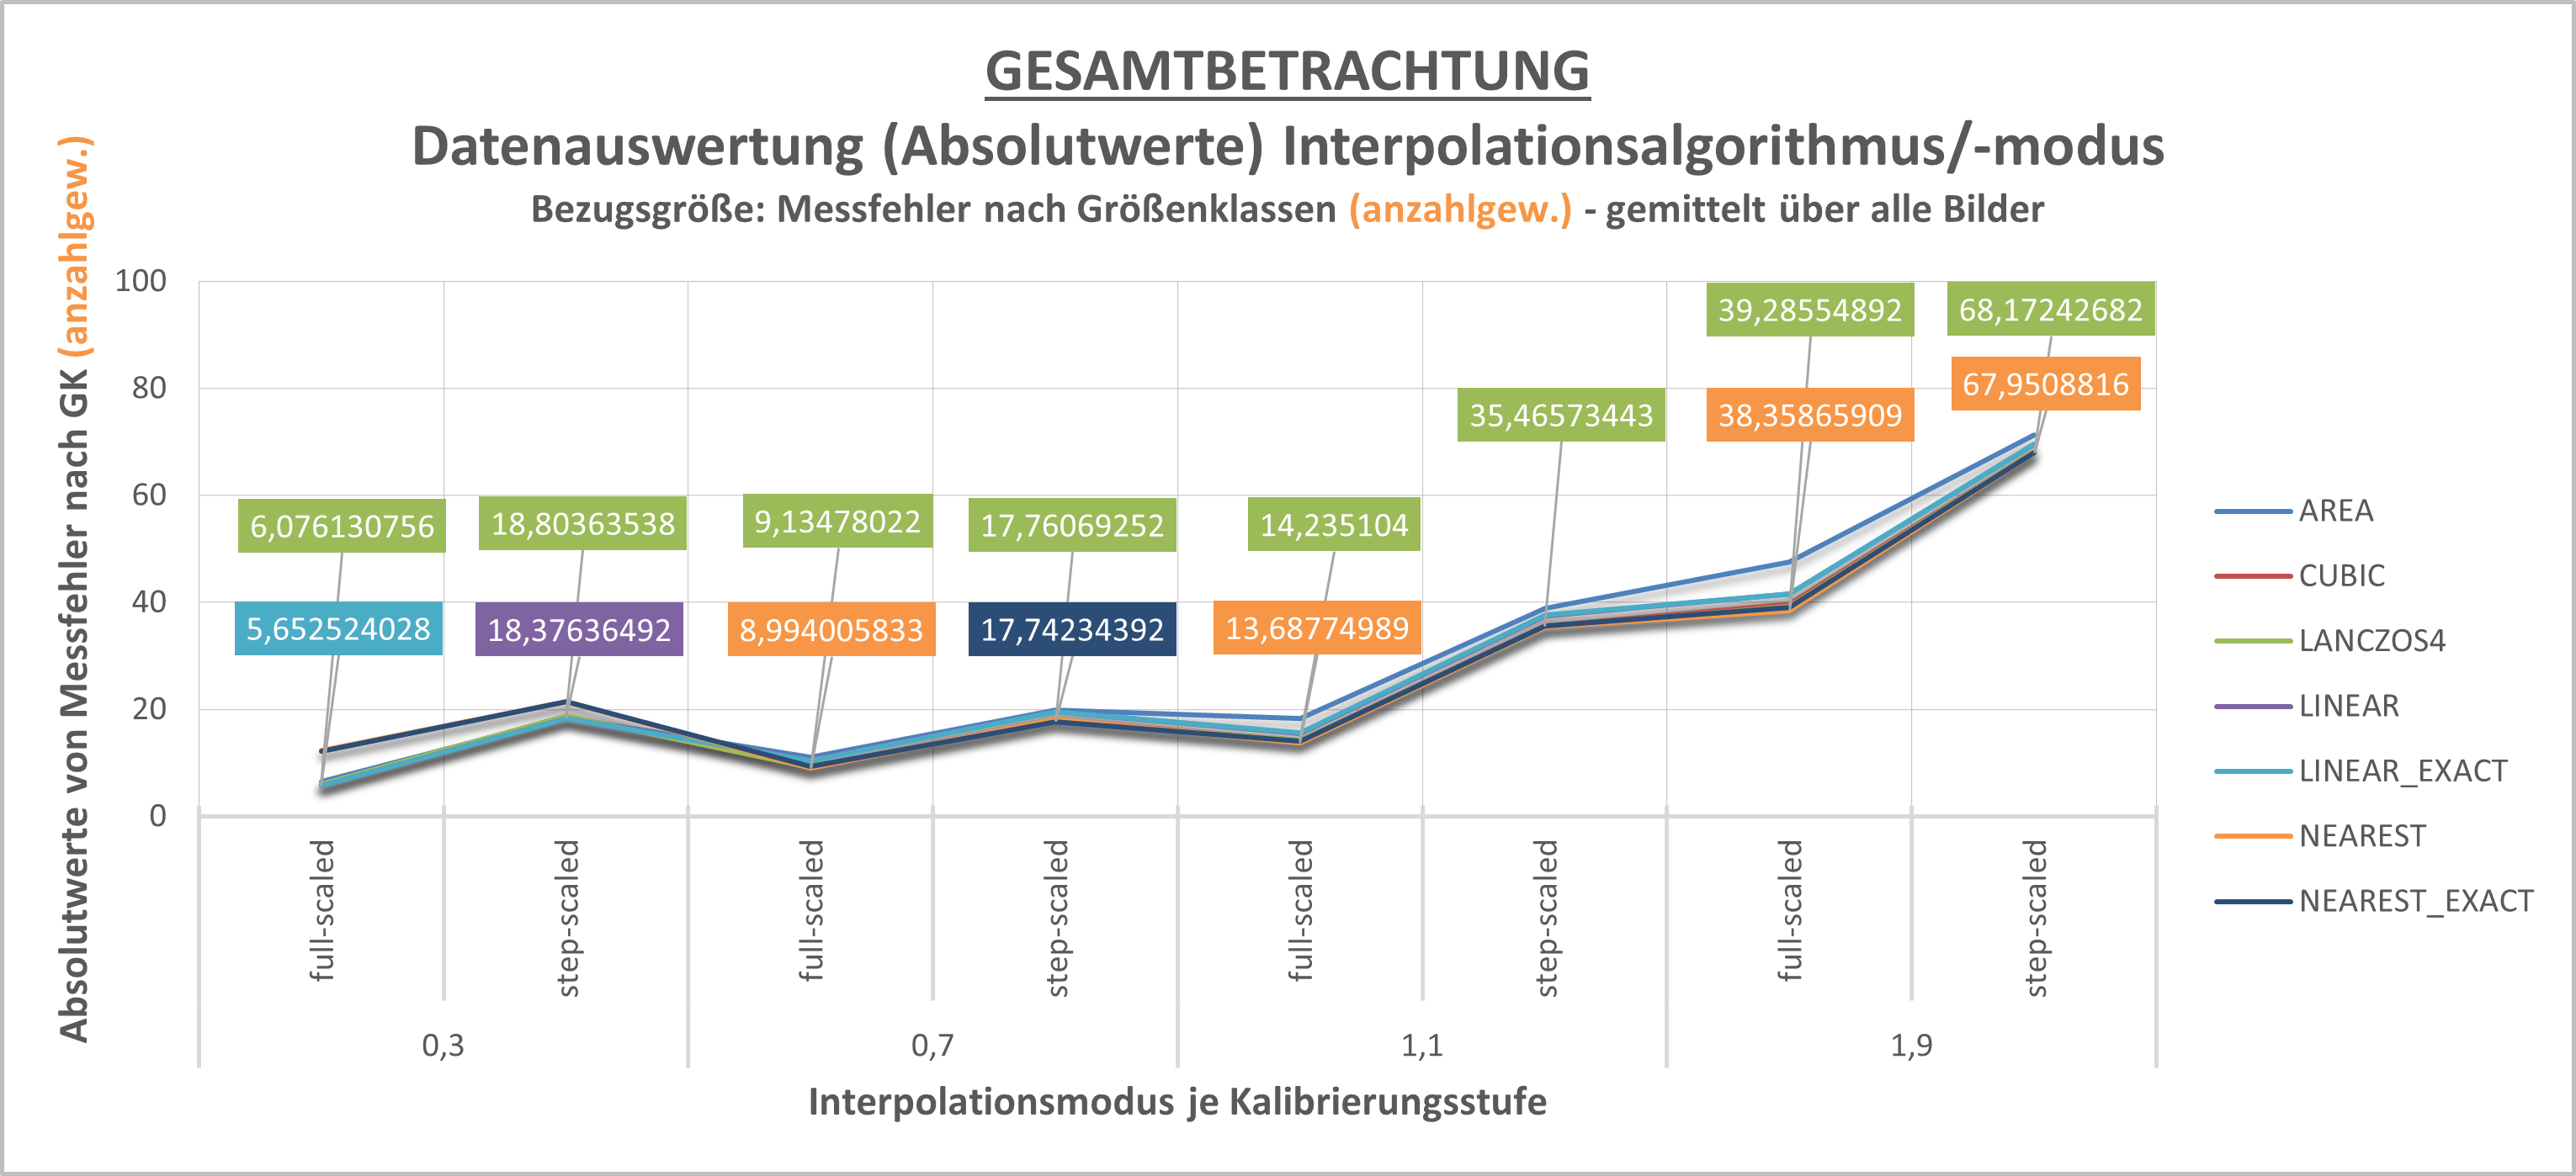
\includegraphics[width=11cm, height=\textheight, keepaspectratio]{pics/DA_Gesamt_Absolut_GKanzahl}
	\caption{Auswertung des Messfehlers (Gesamt) nach Größenklassen (anzahlgewichtet)}
	\label{fig:DAGesamtAbsolutGKanzahl}
\end{figure}

\begin{table}[H]
	\centering
	\caption{Daten zu den berechneten Messfehlern nach Größenklassen (anzahlgewichtet)}
	\label{tab:DAGesamtAbsolutGKanzahl}
	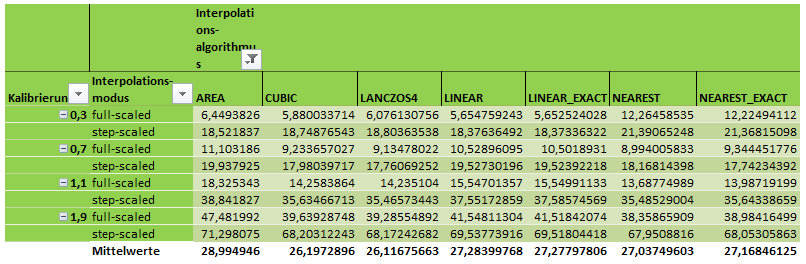
\includegraphics[width=\textwidth, height=\textheight, keepaspectratio]{pics/Tab_DA_Gesamt_Absolut_GKanzahl}
\end{table}


\noindent Was sofort auffällt ist, dass die Kurven sich sehr denen aus der Gesamt-Fehlerbetrachtung im letzten Abschnitt ähneln. Auch hier ist eindeutig der Trend zu erkennen, dass der Fehelr sich mit steigender Ausgangskalibrierung vergrößert und das die Fehler bei der schrittweisen Skalierung immer größer ausfallen, als bei Voll-Skalierung. 
\\\\
Wenn auch knapp, weist die LANCZOS4-Interpolation hier mit einem Durchschnittswert von ca. 26,12 den geringsten durchschnittlichen Fehler auf. Allerdings erzeugt dieses Interpolationsverfahren, wie im Diagramm zu erkennen, nur im Bereich von 1,1 $\nicefrac{\mu m}{\text{Pixel}}$ bei schrittweiser Skalierung auch tatsächlich den geringsten absoluten Messfehler, der allerdings höher ist als bei vergleichbarer Voll-Skalierung und daher vernachlässigbar. Die jeweils kleinsten Werte sind in der dem jeweiligen Algorithmus zugeordneten Diagrammfarbe entsprechend gekennzeichnet. Man kann daran gut erkennen das die Frage danach, welcher Algorithmus denn in dieser Größenklasse den kleinsten Fehler erzeugt, noch nicht hinreichend beantwortet werden kann.
\\\\
Anhand der Streuungsparameter erkennt man, dass die LANCZOS4-Interpolation, wenn auch den geringsten absoluten Fehler, in den meisten Fällen nicht auch die geringste Varianz besitzt wie man in der Abbildungen \ref{fig:DAGesamtStreu1GKanzahl} und \ref{fig:DAGesamtStreu2GKanzahl} i.V.m  den dazugehörigen Datentabellen \ref{tab:DAGesamtStreu1GKanzahl} und \ref{tab:DAGesamtStreu2GKanzahl} eindeutig ablesen kann.

\begin{figure}[H]
	\centering
	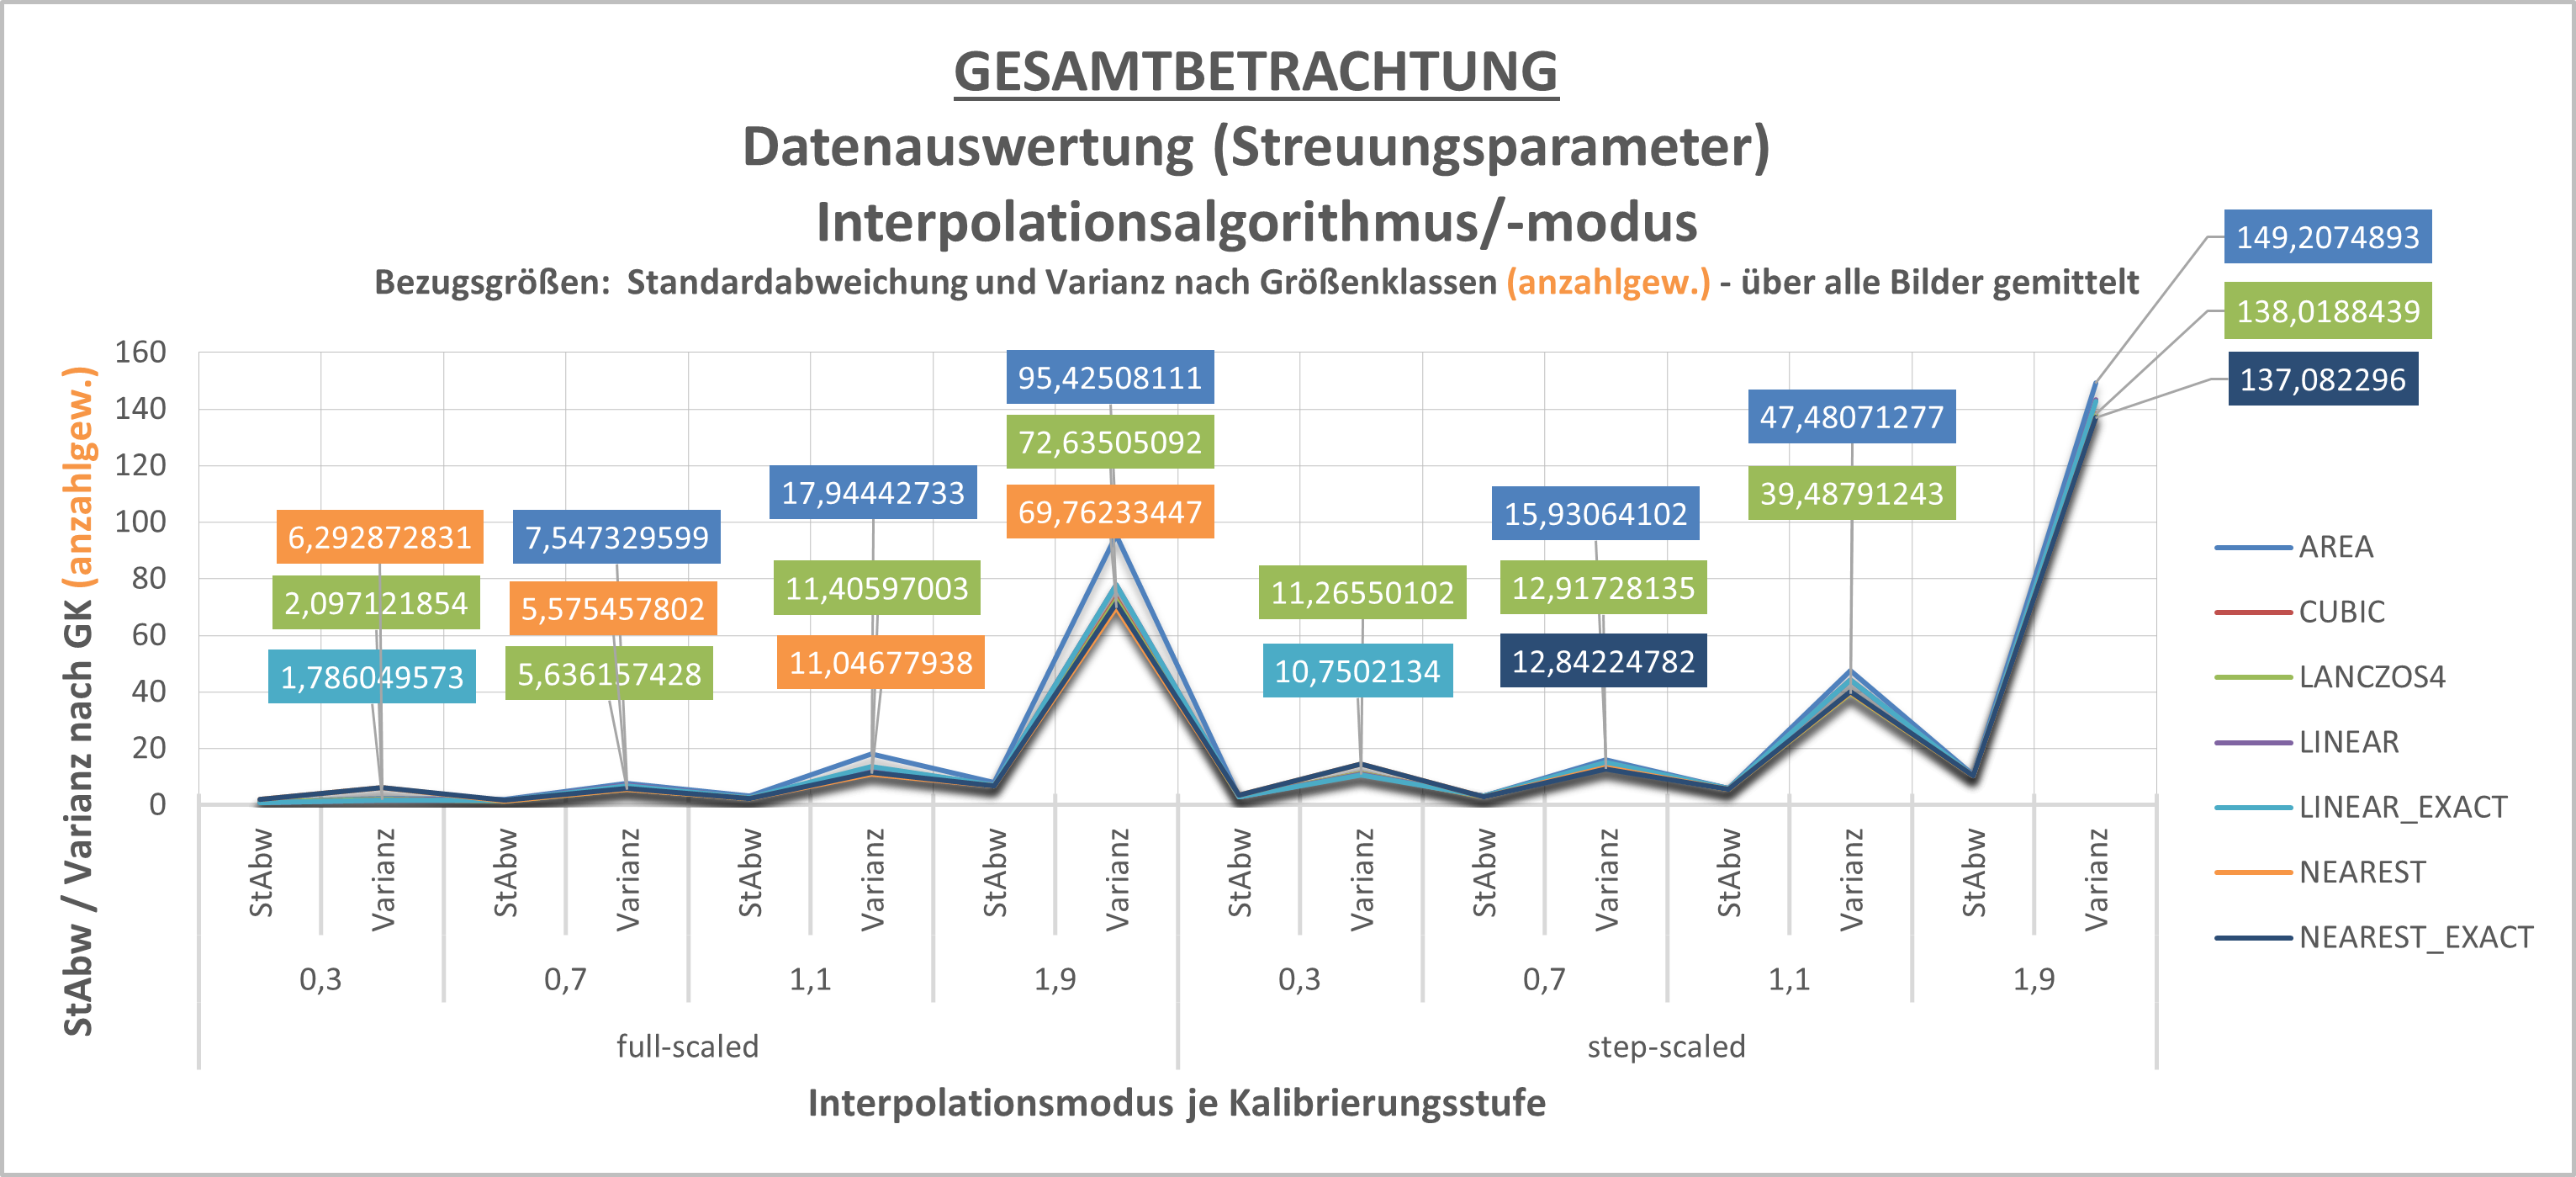
\includegraphics[width=11cm, height=\textheight, keepaspectratio]{pics/DA_Gesamt_Streu1_GKanzahl}
	\caption{Streuungsparameter (Standardabweichung und Varianz) nach Größenklassen (anzahlgewichtet)}
	\label{fig:DAGesamtStreu1GKanzahl}
\end{figure}

\begin{table}[H]
	\centering
	\caption{Daten zu den berechneten Streuungsparametern (Standardabweichung und Varianz) nach Größenklassen (anzahlgewichtet)}
	\label{tab:DAGesamtStreu1GKanzahl}
	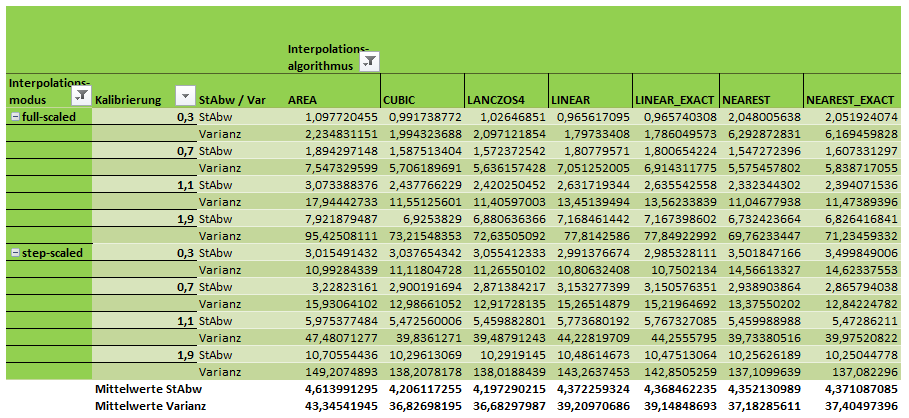
\includegraphics[width=\textwidth, height=\textheight, keepaspectratio]{pics/Tab_DA_Gesamt_Streu1_GKanzahl}
\end{table} 

\begin{figure}[H]
	\centering
	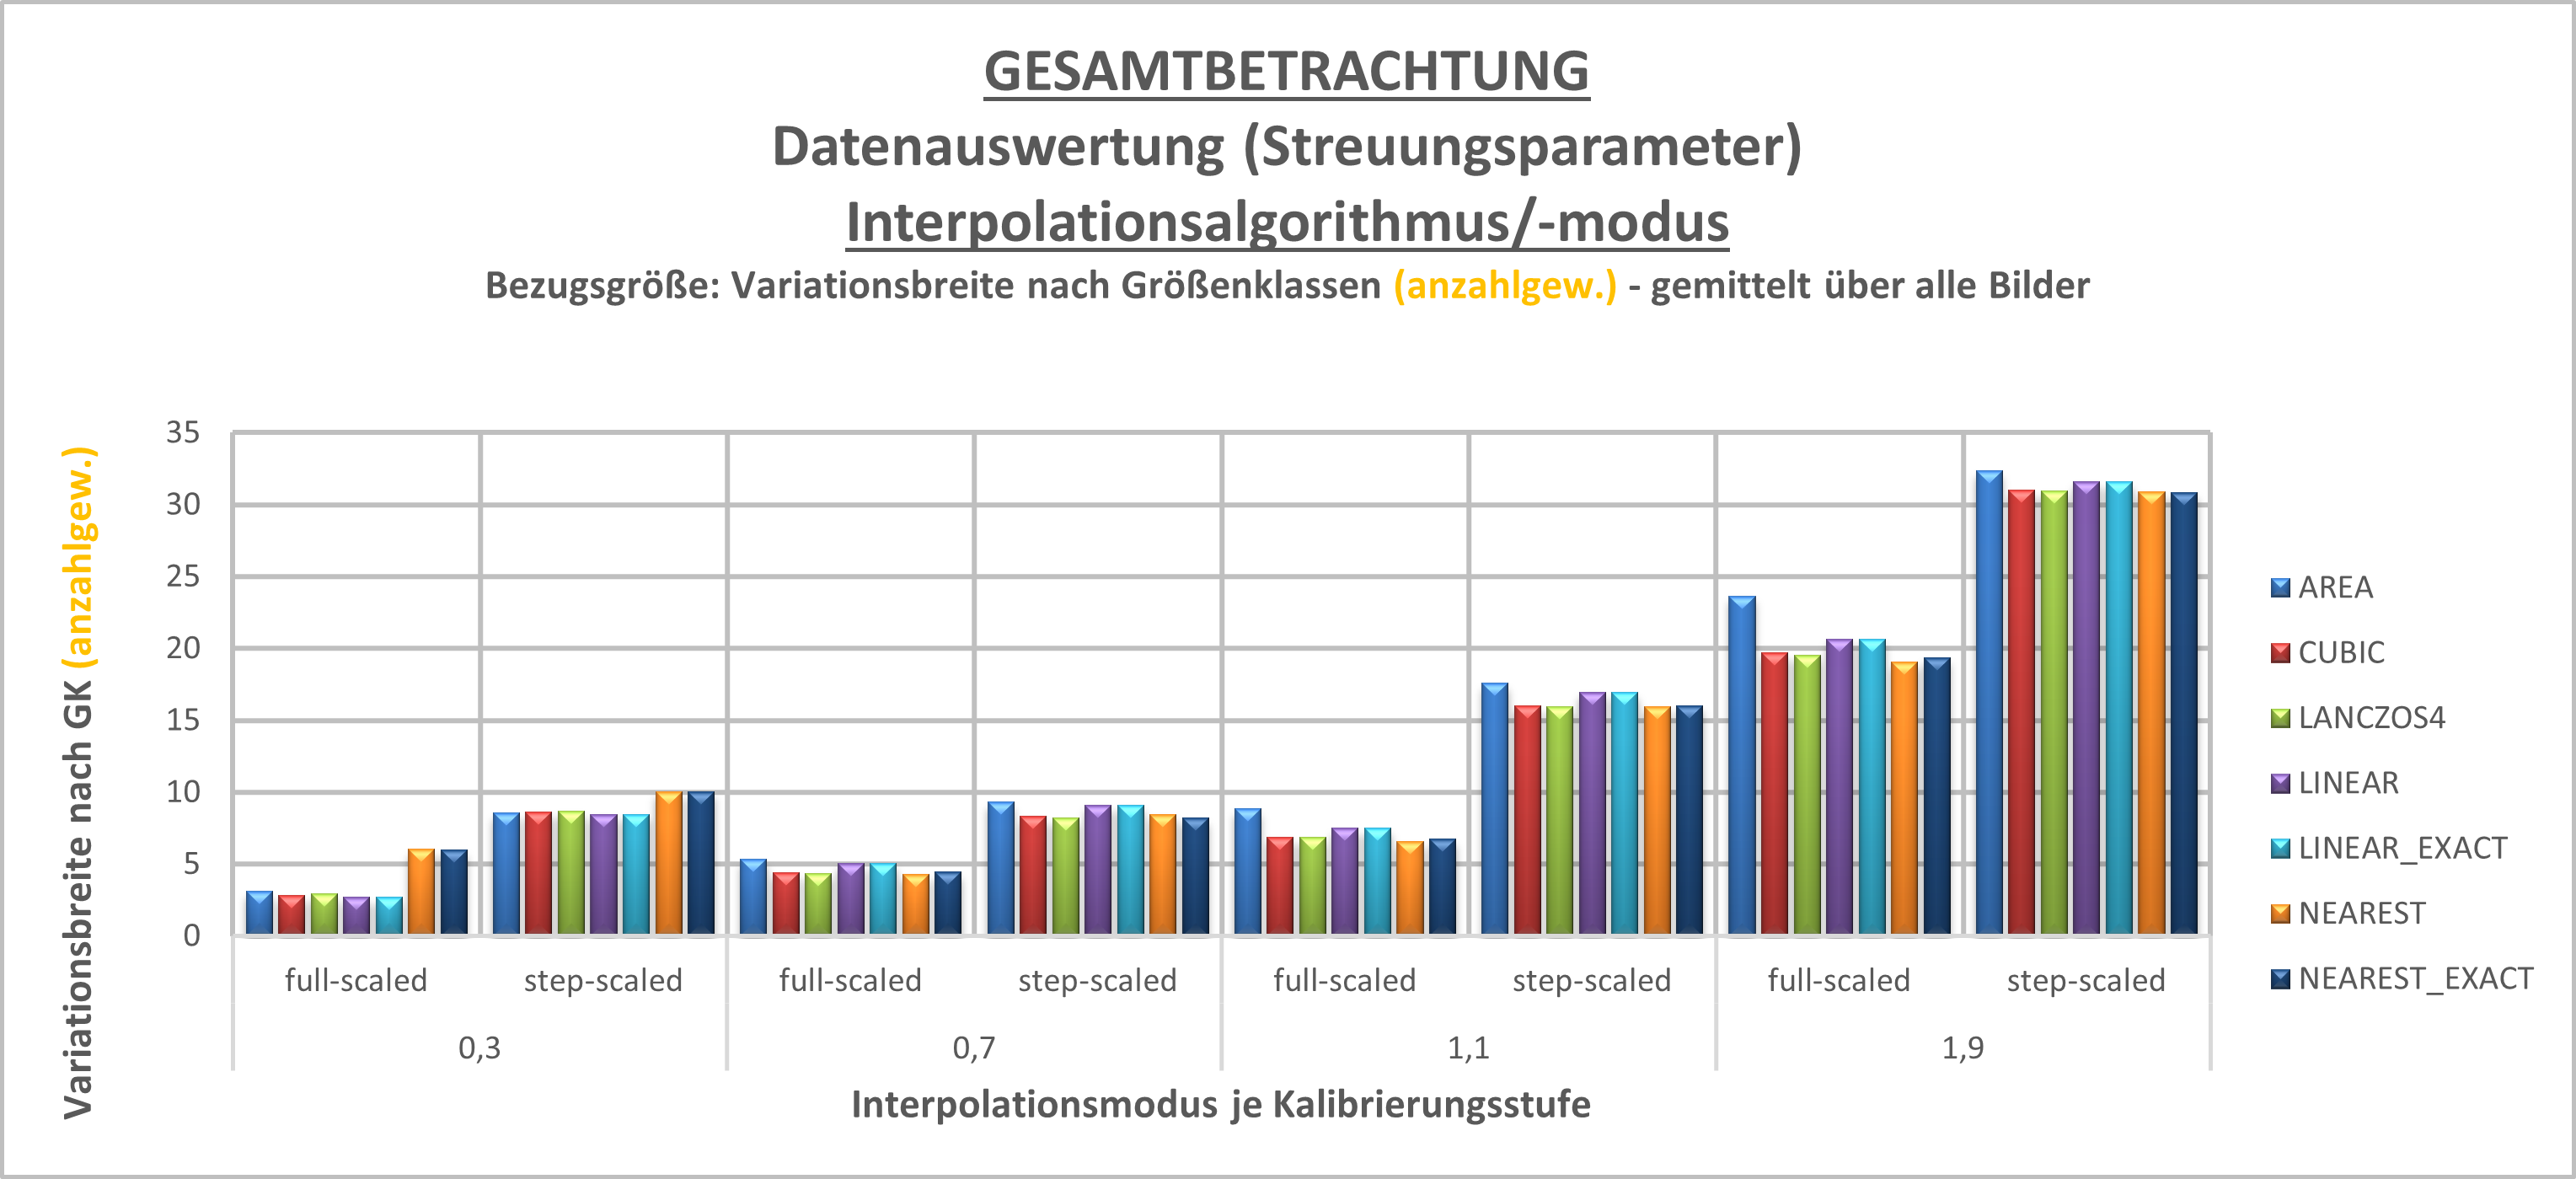
\includegraphics[width=11cm, height=\textheight, keepaspectratio]{pics/DA_Gesamt_Streu2_GKanzahl}
	\caption{Streuungsparameter (Variationsbreite) nach Größenklassen (anzahlgewichtet)}
	\label{fig:DAGesamtStreu2GKanzahl}
\end{figure}

\begin{table}[H]
	\centering
	\caption{Daten zum berechneten Streuungsparameter (Variationsbreite) nach Größenklassen (anzahlgewichtet)}
	\label{tab:DAGesamtStreu2GKanzahl}
	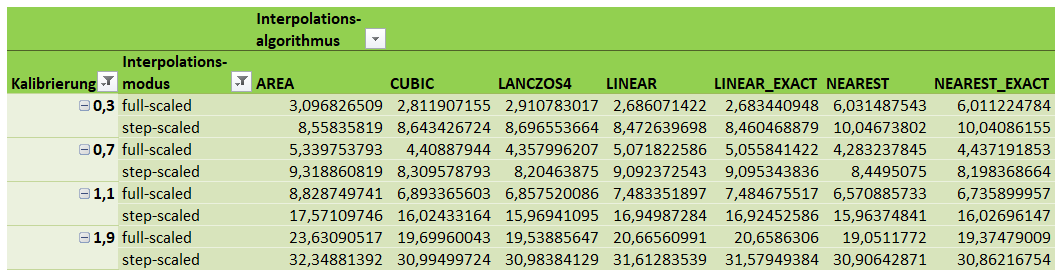
\includegraphics[width=\textwidth, height=\textheight, keepaspectratio]{pics/Tab_DA_Gesamt_Streu2_GKanzahl}
\end{table}

\noindent Das bedeutet, dass die Fehlerstreuung über alle Bilder in den meisten Kalibrierungsstufen für andere Algorithmen geringer ausfällt. Im direkten Vergleich mit der Gesamtauswertung (vgl. Abbildung \ref{fig:DAGesamtStreu1Alle}) sind hier zwar wesentlich geringere Varianzen im Bereich von $0,3~-~1,1\nicefrac{\mu m}{\text{Pixel}}$ (bei Voll-Skalierung) die, unabhängig vom Interpolationsalgorithmus, schon fast vernachlässigbar erscheinen. In der Kalibrierungsstufe $1,9\nicefrac{\mu m}{\text{Pixel}}$ ist hingegen wieder eine sehr hohe Streuung gegeben.
\\\\
\noindent Wie zu Beginn des Abschnitts bereits angekündigt, erfolgt zur vollständigen Betrachtung dieser Größenklassenkategorie nun noch eine Einzelbetrachtung die zeigt, wie sich der Messfehler in den einzelnen Klassen auswirkt (Abbildung \ref{fig:DAEinzelAbsolutGKanzahl}).

\begin{figure}[H]
	\centering
	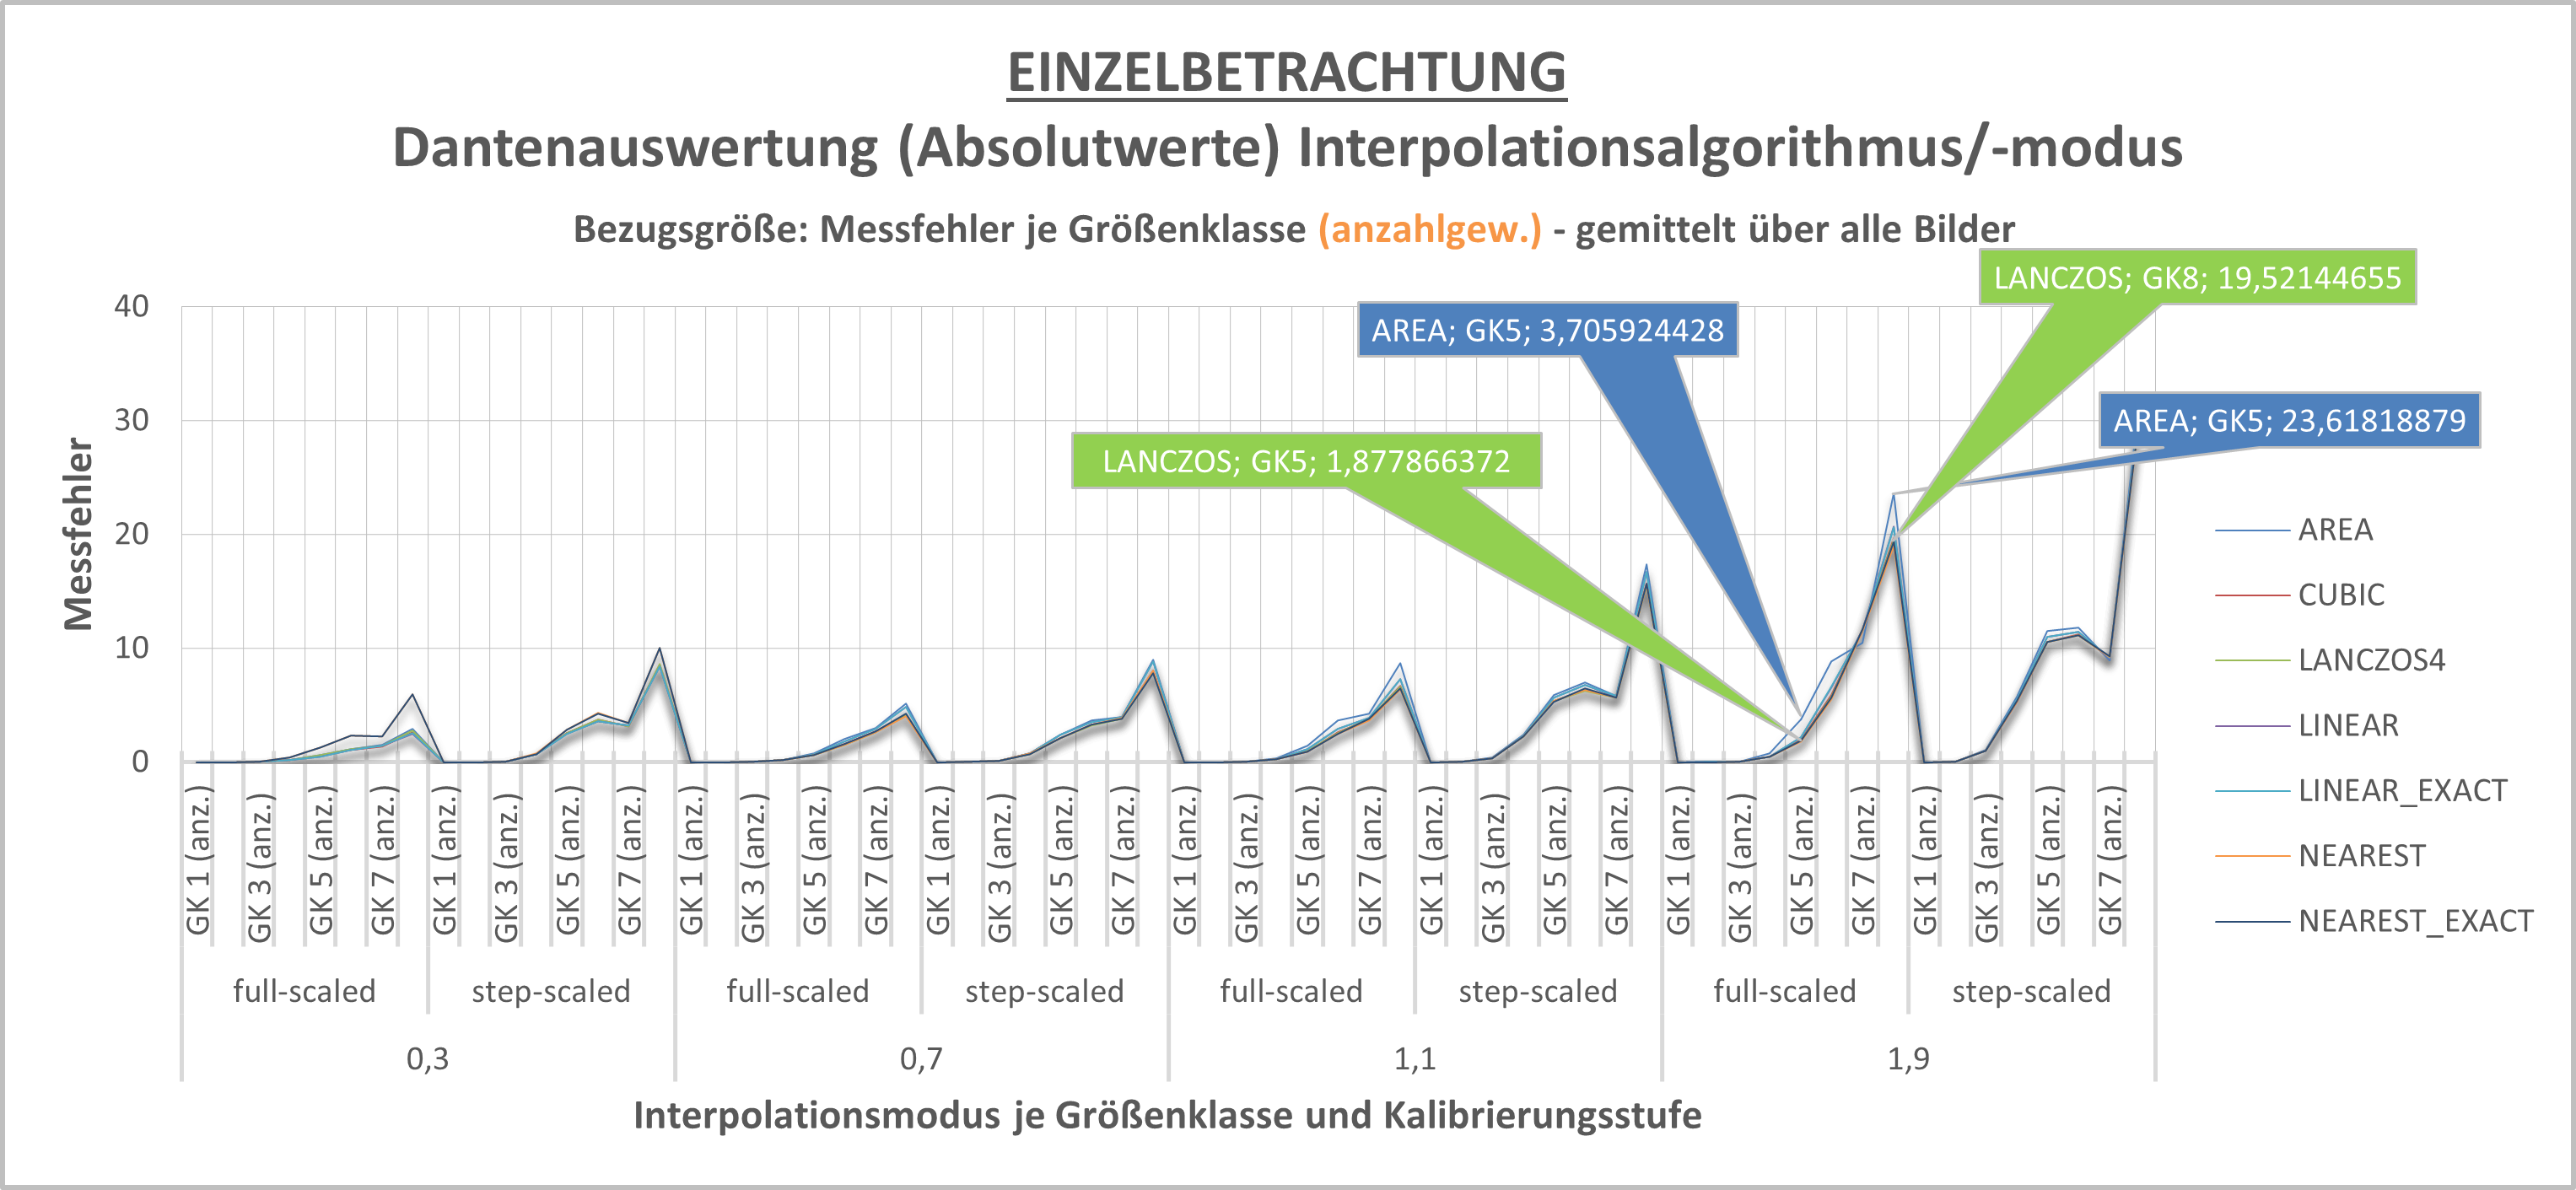
\includegraphics[width=11cm, height=\textheight, keepaspectratio]{pics/DA_Einzel_Absolut_GKanzahl}
	\caption{Auswertung des Messfehlers je Größenklasse im Bereich Größenklassen (anzahlgewichtet)}
	\label{fig:DAEinzelAbsolutGKanzahl}
\end{figure}

\noindent Auch wenn sich die Interpolationsalgorithmen sowohl in der Datenbasis als auch visuell im Diagramm kaum unterscheiden lassen, können hier wichtige Zusammenhänge abgeleitet werden. Die wichtigsten Unterscheidungsmerkmale sind außerdem farblich gekennzeichnet. Im Durchschnitt erzeugt LANCZOS4 über alle Kategorien den kleinsten Messfehler, wobei sich ein etwas anderes Bild ergibt, wenn man nach Größenklassen differenziert.
\\\\
Beispielsweise fällt beim Vergleich von LANCZOS und flächenbasierter Interpolation auf, dass der Messfehler über alle Kalibrierungsstufen in den Größenklassen 1-3 nahezu gegen Null geht, wohingegen in den Kategorien 4-8 ein starker Anstieg beobachtbar ist.Die LANCZOS-Interpolation weist etwa in der Größenklasse 8 mit 19,52 einen mehr als 10 mal höheren Fehlerwert auf, als in der Größenklasse 5 mit ca. 1,88. Bei der flächenbasierten Interpolation  ist der Unterschied dagegen, mit Werten von ca. 3,71 in Größenklasse 5 sowie 23,62 in Klasse 8, etwas geringer, den hier beträgt das Verhältnis mit ca. 6,4 nur etwas mehr als die Hälfte. 
\\\\
Da dieses Beispiel mit LANCZOS und flächenbasierter Interpolation nicht zufällig gewählt wurde, sondern auf der Grundlage einer vorhergehenden Datenanalyse, kann der hier dargestellte Zusammenhang auf alle Kalibrierungsstufen übertragen werden. Auch an der Wiederholung des Musters in der Kurve lässt sich dies sehr gut erkennen. 
\\\\
\colorbox{gray!10}{
	\label{box:ErgebnisGesamtauswertung}
	\begin{minipage}{0.975\textwidth}
		\textbf{\underline{Ergebnis der Auswertung nach Größenklassen (anzahlgewichtet):}}
		\\\\
		Zusammenfassend kann für diesen Abschnitt festgehalten werden, dass die LANCZOS4-Interpolation mit einem Wert von 26,12 zwar über alle Bereiche zwar den kleinsten durchschnittlichen Fehler erzeugt, jedoch nur im Kalibrierungsbereich von 1,1 $\nicefrac{\mu m}{\text{Pixel}}$ bei schrittweise Skalierung auch tatsächlich den kleinsten absoluten Messfehler. Die Streuungsparameter zeigen jedoch das die LANCZOS-Interpolation nicht immer die niedrigste Varianz in den Daten aufweist, sondern nur im Bereich von 0,7 $\nicefrac{\mu m}{\text{Pixel}}$.
		\\\\
		Auch bezogen auf die Größenklassen bestätigt sich die bereits im Abschnitt \ref{subsubsec:AuswertungGesamtfehlerbetrachtung} Beobachtung, dass durch Voll-Skalierung im wesentlich geringere Fehler erzeugt werden, als bei vergleichbarer schrittweisen Skalierung.
		Ein signifikanter Anstieg ist ab einer Kalibrierungsstufe von 1,1 $\nicefrac{\mu m}{\text{Pixel}}$ erkennbar. Jedoch gilt dies nur für die Größenklassen 4-8, wobei die Fehler in den Klassen 1-3 über alle Kalibrierungsstufen und Interpolationsalgorithmen vergleichsweise vernachlässigbar gering ausfallen.
	\end{minipage}
}
\\\\\\

\subsubsection{Auswertung nach Größenklassen (flächengewichtet)}
\label{subsubsec:AuswertungGKflaeche}
Wie schon bei den Größenklassen im vorherigen Abschnitt, teilen sich diese wiederum auf in unterschiedliche Kategorien 1-8. Die Auswertung in diesem Abschnitt erfolgt mit denselben statistischen Methoden, um eine größtmögliche Vergleichbarkeit zu gewährleisten.
\\\\
\noindent Abbildung \ref{fig:DAGesamtAbsolutGKflaeche} sowie die Datentabelle \ref{tab:DAGesamtAbsolutGKflaeche} zeigen zunächst wieder das Gesamtbild der Datenverteilung in den unterschiedlichen Kalibrierungsstufen.

\begin{figure}[H]
	\centering
	\includegraphics[width=11cm, height=\textheight, keepaspectratio]{pics/DA_Gesamt_Absolut_GKfläche}
	\caption{Auswertung des Messfehlers (Gesamt) nach Größenklassen (flächengewichtet)}
	\label{fig:DAGesamtAbsolutGKflaeche}
\end{figure}

\begin{table}[H]
	\caption{Messdaten zur Auswertung des Messfehlers (Gesamt) nach Größenklassen (flächengewichtet)}
	\label{tab:DAGesamtAbsolutGKflaeche}
	\begin{figure}[H]
		\centering
		\includegraphics[width=\textwidth, height=\textheight, keepaspectratio]{pics/Tab_DA_Gesamt_Absolut_GKfläche}
	\end{figure}
\end{table}

\noindent Im Vergleich mit den Größenklassen (anzahlgewichtet) ist hier ein ganz ähnlicher Verlauf zu erkennen, allerdings ist es nun die kubische Interpolation (rote Datenpunkte), die mit einem gemittelten Wert von ca. 28,73 über alle Bereiche den geringsten Fehler erzeugt. Jedoch ergibt sich auch wieder ein etwas anderes Bild, wenn man untersucht, für welche Kategorien das letztendlich auch wirklich zutrifft. Die Abbildung zeigt daher jeweils auch die minimalen Werte an, außer in den Fällen in denen die kubische Interpolation tatsächlich auch den geringsten Fehler aufweist. 
\\\\
\noindent Die Streuungsparameter Standardabweichung und Varianz zeigen auf den ersten Blick nahezu exakt den selben Verlauf wie in Abschnitt \ref{subsubsec:AuswertungGKanz}, allerdings sind auch unterschiedliche Algorithmen für die jeweils größten und kleinsten Fehler verantwortlich (Abbildung \ref{fig:DAGesamtStreu1GKfläche} i.V.m. Datentabelle \ref{tab:DAGesamtStreu1GKflaeche} sowie Abbildung \ref{fig:DAGesamtStreu2GKfläche} und Datentabelle \ref{tab:DAGesamtStreu2GKflaeche}).

\begin{figure}[H]
	\centering
	\includegraphics[width=11cm, height=\textheight, keepaspectratio]{pics/DA_Gesamt_Streu1_GKfläche}
	\caption{Streuungsparameter (Standardabweichung u. Varianz) nach Größenklassen (flächengewichtet)}
	\label{fig:DAGesamtStreu1GKfläche}
\end{figure}

\begin{table}[H]
	\caption{Daten zu den berechneten Streuungsparametern (Standardabweichung u. Varianz) nach Größenklassen (flächengewichtet)}
	\label{tab:DAGesamtStreu1GKflaeche}
	\begin{figure}[H]
		\centering
		\includegraphics[width=\textwidth, height=\textheight, keepaspectratio]{pics/Tab_DA_Gesamt_Streu1_GKfläche}
	\end{figure}
\end{table}

\begin{figure}[H]
	\centering
	\includegraphics[width=14cm, height=\textheight, keepaspectratio]{pics/DA_Gesamt_Streu2_GKfläche}
	\caption{Streuungsparameter (Variationsbreite) nach Größenklassen (flächengewichtet)}
	\label{fig:DAGesamtStreu2GKfläche}
\end{figure}

\begin{table}[H]
	\caption{Daten zum berechneten Streuungsparameter (Variationsbreite) nach Größenklassen (flächengewichtet)}
	\label{tab:DAGesamtStreu2GKflaeche}
	\begin{figure}[H]
		\centering
		\includegraphics[width=\textwidth, height=\textheight, keepaspectratio]{pics/Tab_DA_Gesamt_Streu2_GKfläche}
	\end{figure}
\end{table}

\noindent Während die Standardabweichung mit einem Wert von im Mittel ca. 4,35 und einer Variationsbreite von gerade mal ca. 0,42 sehr gering ist und kaum schwankt, zeigen die Varianzen wieder, dass die kubische Interpolation in fast allen Bereichen nur mittelmäßig abschneidet. Das ist an den eingezeichneten minimalen und maximalen Datenpunkten zu erkennen, denn nur im Bereich von 1,1 $\nicefrac{\mu m}{\text{Pixel}}$ (schrittweise Skalierung) weist die kubische Interpolation auch tatsächlich die geringste Varianz auf.
\\\\
\noindent Zur Vervollständigung der Analyse in diesem Bereich, folgt nun wieder eine Einzelbetrachtung der Größenklassen (flächengewichtet). In der nachstehenden Abbildung \ref{fig:DAEinzelAbsolutGKflaeche} ist zu erkennen, dass wiederum in den Klassen 4-8 ein signifikanter Anstieg der Fehlerwerte vorliegt.

\begin{figure}[H]
	\centering
	\includegraphics[width=14cm, height=\textheight, keepaspectratio]{pics/DA_Einzel_Absolut_GKfläche}
	\caption{Auswertung des Messfehlers (Einzel) nach Größenklassen (flächengewichtet)}
	\label{fig:DAEinzelAbsolutGKflaeche}
\end{figure}

\noindent Für den im Diagramm eingezeichneten Vergleich (rote Datenpunkte) wurde die kubische Interpolation gewählt, weil bei diesem Interpolationsverfahren über alle Größenklassen der geringste durchschnittliche Messfehler auftritt. Dabei ist festzustellen, das bspw. wie hier in Kalibrierungsstufe 1,9 $\nicefrac{\mu m}{\text{Pixel}}$ (Vollskalierung), der Fehlerwert in Größenklasse 8 mit ca. 10,87 nur etwa 3,4 mal höher ist als in Klasse 5 mit ca. 3,15. Außerdem ist sowohl bei Voll- als auch bei der schrittweisen Skalierung jeweils ein Knick in der im Bereich der Größenklasse 7 auffällig, bei dem die Fehlerwerte im verglichen mit Klasse 6 zunächst absinken und dann wieder sehr stark ansteigen. 
\\\\
\colorbox{gray!10}{
	\label{box:Ergebnis der Auswertung nach Größenklassen (flächengewichtet):}
	\begin{minipage}{0.975\textwidth}
		\textbf{\underline{Ergebnis der Auswertung nach Größenklassen (flächengewichtet):}}
		\\\\
		Es wurde in diesem Teil der Analyse festgestellt, dass die kubische Interpolation mit einem  Fehler von 28,72 einen über alle Bereiche geringsten durchschnittlichen Wert aufweist, aber nur im bei Kalibrierung von 0,7 $\nicefrac{\mu m}{\text{Pixle}}$ bei Voll-Skalierung auch den tatsächlich kleinsten absoluten Wert. Die Streuungsparameter zeigen bei einer konstant sehr niedrigen Standardabweichung, dass bei der die kubischen Interpolation nur im Bereich 1,1 $\nicefrac{\mu m}{\text{Pixel}}$ auch die kleinste Varianz in den Daten gegeben ist.
		\\\\
		Wie auch an früherer Stelle schon festgestellt gilt auch hier wieder, dass die Verkleinerung von Bildern geringere Fehler erzeugt, als die Vergrößerung. Bedeutende Anstiege des Fehlers ist auch hier ab Kalibrierungsstufe 1,1 $\nicefrac{\mu m}{\text{Pixel}}$ gegeben, was jedoch wieder nur für die Größenklassen 4-8 zutreffend ist.
	\end{minipage}
}
	
\subsubsection{Auswertung nach Anordnungsklassen}

Die Bestimmung der Anordnungsklassen ist ebenfalls ein von der Software AMGuss bei Durchführung einer Lamellengraphitauswertung zurückgegebenes Ergebnis, bei dem die Häufigkeiten der gefundenen Anordnungsklassen (vgl. auch Bild \ref{fig:Anordnungsklassen} auf Seite \pageref{fig:Anordnungsklassen}) auch in einem Histogramm dargestellt werden.  Diese Kategorie soll nun abschließend ebenfalls eingehend untersucht werden und im Anschluss daran alle Teilergebnisse zu einer Gesamtauswertung zusammengefasst werden.
\\\\
\noindent Die nachstehende Abbildung \ref{fig:DAGesamtAbsolutAKL} i.V.m. Datentabelle \ref{tab:DAGesamtAbsolutAKL} zeigen an, dass die LANCZOS4-Interpolation mit einem durchschnittlichen absoluten Fehlerwert über alle Bilder den geringster Fehler verursacht. Doch bei genauerer Betrachtung stellt sich heraus, dass dies in keinem Bereich dem tatsächlich geringsten absoluten Fehler entspricht. 

\begin{figure}[H]
	\centering
	\includegraphics[width=11cm, height=\textheight, keepaspectratio]{pics/DA_Gesamt_Absolut_AKL}
	\caption{Auswertung des Messfehler nach Anordnungsklassen}
	\label{fig:DAGesamtAbsolutAKL}
\end{figure}

\begin{table}[H]
	\caption{Messdaten zur Auswertung des Messfehler nach Anordnungsklassen}
	\begin{figure}[H]
		\centering
		\includegraphics[width=\textwidth, height=\textheight, keepaspectratio]{pics/Tab_DA_Gesamt_Absolut_GKfläche}
		\label{tab:DAGesamtAbsolutAKL}
	\end{figure}
\end{table}

Zu erkennen ist das wieder an den farbig markierten Datenpunkten die ebenfalls angeben, welcher Algorithmus in der jeweiligen Kategorie den geringsten Wert aufweist. Wie man unschwer erkennen kann, ergibt sich auch hier wieder ein sehr unklares Bild, da der Algorithmus, welcher über aller Bilder den geringsten durchschnittlichen Fehler in dieser Kategorie aufweist, nicht derselbe ist, der in den unterschiedlichen Kalibrierungsstufen und Interpolationsmodi auch zum geringsten Fehler führt - und zwar in keinem einzigen Bereich.
\\\\
Die Streuungsparameter zeigen ebenfalls hohe Varianzen an, 

\begin{figure}[H]
	\centering
	\includegraphics[width=14cm, height=\textheight, keepaspectratio]{pics/DA_Gesamt_Streu1_AKL}
	\caption{Streuungsparameter (Standardabweichung u. Varianz) nach Anordnungsklassen}
	\label{fig:DAGesamtStreu1AKL}
\end{figure}

\begin{table}[H]
	\caption{Daten zu den berechneten Streuungsparametern (Standardabweichung u. Varianz) nach Anordnungsklassen}
	\begin{figure}[H]
		\centering
		\includegraphics[width=\textwidth, height=\textheight, keepaspectratio]{pics/Tab_DA_Gesamt_Streu1_AKL}
		\label{tab:DAGesamtStreu1GAKL}
	\end{figure}
\end{table}

\begin{figure}[H]
	\centering
	\includegraphics[width=14cm, height=\textheight, keepaspectratio]{pics/DA_Gesamt_Streu2_AKL}
	\caption{Streuungsparameter (Variationsbreite) nach Anordnungsklassen}
	\label{fig:DAGesamtStreu2AKL}
\end{figure}

\begin{table}[H]
	\caption{Daten zum berechneten Streuungsparameter (Variationsbreite) nach Anordnungsklassen}
	\begin{figure}[H]
		\centering
		\includegraphics[width=\textwidth, height=\textheight, keepaspectratio]{pics/Tab_DA_Gesamt_Streu2_AKL}
		\label{tab:DAGesamtStreu2GAKL}
	\end{figure}
\end{table}

\begin{figure}[H]
	\centering
	\includegraphics[width=14cm, height=\textheight, keepaspectratio]{pics/DA_Einzel_Absolut_AKL}
	\caption{Auswertung des Messfehlers (Einzel) nach Anordnungsklassen}
	\label{fig:DAEinzelAbsolutAKL}
\end{figure}

Auf Daten wird hier aus Darstellungsgründen verzichtet...

\chapter{Zusammenfassung und Auswertung}

\section{Zusammenfassung}

\section{Auswertung}


\bibliographystyle{IEEEtran}
\bibliography{literature}



\end{document}